\seccion{Algunos ejemplos de distribuciones de probabilidad}
\label{Sec:MP:EjemplosDistribucionesProb}

En esta secci\'on, vamos a ver unos ejemplos de distribuciones que se encuentran
frecuentemente   en   problema   pr\'acticos   de   varias   areas   cientificas
(estad\'istica, f\'isica,  ingener\'ia,\ldots).  Daremos las  caracteristicas de
cada ley presentada, as\'i que sus propiedades remarcables. El num\'ero de leyes
de probababilidad es tan importante que es dificil, para no decir imposible, ser
exahustivo. Adem\'as, existen muchas  relaciones entre leyes. En esta secci\'on,
vamos  a  ver algunas  leyes  que  aparecen  frecuentemente, y  nos  enfocaremos
solamente sobre  algunos v\'inculos entre  leyes (los principales).   Para tener
m\'as detalles,  se puede referirse a  los libros especializados  en este marco,
como  por  ejemplo~\cite{Spi76,  JohKot92, JohKot97,  JohKot95:v1,  JohKot95:v2,
KotBal00, GupNag99, FanKot90, SamTaq94}.

\

\modif{
Usaremos a veces en el resto de  este libro la notaci\'on $\sim$ para decir ``la
variable  aleatoria   es  distribuida   de  acuerdo   a  la   distribuci\'on  de
probabilidad'', ej. $X \sim p_X$ o $X \sim \N$ (ver m\'as adelante).}


% ================================= Variables discretas
\subseccion{Distribuciones de variable discreta}
\label{Ssec:MP:EjemplosDistribucionesDiscretas}


% --------------------------------- Certeza
\subsubseccion{Variable real con certeza}
\label{Sssec:MP:Certeza}

El caso \ $X = a \in \Rset^d$ \ deterministico ($\forall \, \omega, \: X(\omega)
= a$)  puede ser ver  visto como un  caso degenerado de vector  aleatorio. Visto
as\'i, sus caracter\'isticas principales  vistas en las secciones anteriores son
resimidas en la tabla siguiente:

\begin{caracteristicas}
%
Dominio de definici\'on & $\X = \{ a \}, \quad a \in \Rset^d$\\[2mm]
\hline
%
Distribuci\'on de probabilidad & $p_X(x) = \un_{\{a\}}(x)$\\[2mm]
\hline
%
Promedio & $\displaystyle m_X = a$\\[2mm]
\hline
%
Covarianza~\footnote{Siendo cero la covarianza, no se define ni la asimetr\'ia,
ni la curtosis. Sin embargo, de una manera se puede decir que la ley no es
asim\'etrica, y con cola livianas (no hay colas).} & $\displaystyle \Sigma_X =
0$\\[2mm]
\hline
%
%\modif{Asimetr\'ia} & $\gamma_X = 0$\\[2mm]
%\hline
%%
%Curtosis por exceso & $\displaystyle \widebar{\kappa}_X = - \sum_{i,j=1}^d \Big( \! \left(
%    \un_i \un_i^t \right) \otimes \left(  \un_j \un_j^t \right) +  \left( \un_i
%    \un_j^t \right) \otimes \left( \un_i  \un_j^t \right) + \left( \un_i \un_j^t
%  \right) \otimes \left( \un_j \un_i^t \right) \! \Big)$\\[2mm]
%\hline
%
Generadora de probabilidad & $\displaystyle G_X(z) = \prod_{i=1}^d z_i^{a_i}$ \ para \ $z_i \in \Cset$
\ si $a_i \ge 0$ \ y \ $\Cset^*$ \ si no\\[2mm]
\hline
%
Generadora de momentos & $\displaystyle M_X(u) = e^{a^t u}$ \ para \ $u \in
\Cset^d$\\[2mm]
\hline
%
Funci\'on caracter\'istica & $\displaystyle \Phi_X(\omega) = e^{\imath \, a^t
\omega}$
\end{caracteristicas}

% Momentos & $ \Esp\left[ X^k \right] = p^k$\\[2mm]
% Momento factorial & $\Esp\left[ (X)_k \right] = ?$\\[2mm]

La funci\'on de masa y funci\'on de repartici\'on son representadas en la figura
Fig.~\ref{Fig:MP:Certeza} en el caso escalar.
%
\begin{figure}[h!]
\begin{center} \begin{tikzpicture}%[scale=.9]
\shorthandoff{>}
%
\pgfmathsetmacro{\a}{2};% a
\pgfmathsetmacro{\sy}{2.5};% y-scaling
\pgfmathsetmacro{\r}{.05};% radius arc non continuity F_X
%
% masa
\begin{scope}
%
%
\draw[>=stealth,->] (-.3,0)--({\a+1.75},0) node[right]{\small $x$};
\draw[>=stealth,->] (0,-.1)--(0,{\sy+.25}) node[above]{\small $p_X$};
%
\draw[dotted] (\a,0)--(\a,\sy) node[scale=.4]{$\bullet$};
\draw (0,\sy)--(-.1,\sy) node[left,scale=.7]{$1$};
\draw (0,0)--(0,-.1) node[below,scale=.7]{$0$};
\draw (\a,0)--(\a,-.1) node[below,scale=.7]{$a$};
%
\node at ({(\a+1.75)/2},-1) [scale=.9]{(a)};
\end{scope}
%
%
% reparticion
\begin{scope}[xshift=8.5cm]
%
\draw[>=stealth,->] (-.3,0)--({\a+1.75},0) node[right]{\small $x$};
\draw[>=stealth,->] (0,-.1)--(0,{\sy+.25}) node[above]{\small $F_X$};
%
% cumulativa
\draw[thick] (-.25,0)--(\a,0);
\draw ({\a+\r},\r) arc (90:270:\r);
\draw[dotted] (\a,0)--(\a,\sy);
\draw[thick] (\a,\sy) node[scale=.4]{$\bullet$}--({\a+1.5},\sy);
%
\draw (0,\sy)--(-.1,\sy) node[left,scale=.7]{$1$};
\draw (\a,0)--(\a,-.1) node[below,scale=.7]{$a$};
%
\node at ({(\a+1.75)/2},-1) [scale=.9]{(b)};
\end{scope}
%
\end{tikzpicture} \end{center}
% 
\leyenda{Ilustraci\'on  de una  distribuci\'on  cierta (a),  y  la funci\'on  de
  repartici\'on asociada (b).}
\label{Fig:MP:Certeza}
\end{figure}

\

Notar que todo se extiende al caso complejo sin costo adicional.

\

\index{Ley de gran n\'umeros}
El caso  de variables  deterministicas puede ser  visto como caso  degenerado de
variables aleatorias, pero aparecen de vez a cuando tambi\'en como caso l\'imite
de  sucesiones o  series  de  variables aleatorias.   En  particular, aparece  a
trav\'es de  la ley  de gran n\'umeros,  un de  los primeros casos  de l\'imites
estudiado tratando  de variables aleatorias. Historicamente, un  de los primeros
que  estudio  la convergencia  (sin  prueba  e  implicitamente) de  un  promedio
empirico a esta ``ley'' es el  matem\'atico italiano y jugador de dados y cartas
Gerolamo Cardano en el siglo~{XVI}, en su libro sobre los juegos de azar escrito
en  1564   (ver  introducci\'on  y~\cite{Car63,   Bel05}  o~\cite[Cap.~4]{Hal90}
o~\cite[Cpa.~3]{Mlo08}).  En  otras palabras,  explic\'o que la  precisi\'on las
estadisticas empiricos se mejora con el  n\'umero de datos, lo que es nada m\'as
que, en palabras,  el resultado de la ley dicha de  gran n\'umeros. En palabras,
saliendo  de  variables  aleatoria  independientes  de misma  ley,  el  promedio
empirico tiende a  la media donde enfatisaremos en que  sentido hay que entender
``tiende a''. Tal  convergencia fue estudiada y probada  mucho m\'as tarde, bajo
el  impulso  del suizo  Jacob  Bernoulli~\cite[Pars  4]{Ber1713} (ver  tambi\'en
Montmort~\cite{Mon13, Pea25})  en el  contexto de variables  binarias, conocidos
hoy  como  variables  de Bernoulli  (ver  subecci\'on~\ref{Sssec:MP:Bernoulli}).
Luego,  el  teorema  fue   mejorado  por  ejemplo  por  de  Moivre~\cite{Moi46},
Laplace~\cite{Lap12} o Poisson~\cite{Poi37}, yendo  m\'as all\'a de solamente la
convergencia del  promedio empirico a la  media.  El teorema  fue ampliado m\'as
all\'a  de la  ley  binomial como  suma  de variables  de  Bernoulli (ver  m\'as
adelante),    por    varios    autores   tales    que    Chebyshev~\cite{Tch46},
Markov~\cite{Mar13},    Borel~\cite{Bor09:12}     ,    Kinchin~\cite{Kin29}    o
Kolmogoroff~\cite{Kol30} entre otros (ver~\cite{Sen13} y referencias).

Formalmente,  las dos  versiones usuales  del  teoremas de  formaliza de  manera
siguiente  (ver  tambi\'en~\cite{Fel71,  Shi84,  AshDol99,  JacPro03,  AthLah06,
  Bil12, Coh13}).

\begin{teorema}[Ley debil de los gran n\'umero]
  Sea  \ $\left\{ X_k  \right\}_{k \in  \Nset^*}$ \  una sucesi\'on  de vectores
  aleatorios  independientes e identicamente  distribuidas (iid),  admitiendo una
  media  $m =  \Esp[X_k]$  \ y  sea  \ $\displaystyle  \widebar{X}_n =  \frac1n
  \sum_{k=1}^n X_k$ \ el promedio empirico. Entonces
  %
  \[
  \widebar{X}_n \limitP{n \to +\infty} m
  \]
  %
  donde $\limitP{}$ significa que el l\'imite es en probabilidad, \ie
  %
  \[
  \forall  \:  \varepsilon  >0,  \quad  \lim_{n  \to  +\infty}  P\left(  \left\|
      \widebar{X}_n - m \right\| > \varepsilon \right) = 0
  \]
\end{teorema}
\begin{proof}
  Una    prueba    sencilla   se    apoya    en    el    teorema   de    Markov,
  Cor.~\ref{Cor:MP:Markov},  cuando  los $X_k$  admiten  una  covarianza. De  la
  independencia, es  sencillo ver que  \ $\Cov\left[ \widebar{X}_n \,  \right] =
  \frac1n \Cov\left[ X_1 \right]$. Entonces,
  %
  \[
  P\left(  \left\|  \widebar{X}_n  -  m  \right\|  >  \varepsilon  \right)  \le
  \frac{\Esp\left[ \left\|  \widebar{X}_n - m\right\|^2 \right]}{\varepsilon^2}
  =  \frac{\Tr\left(   \Cov\left[  X_1  \right]   \right)}{n  \,  \varepsilon^2}
  \xrightarrow[n \to \infty]{} 0
  \]
  %
  lo que cierra la prueba.

  De hecho,  no es necesario  que los $X_k$  admitan una covarianza.  Una prueba
  alternativa    se   apoya   sobre    la   funci\'on    caracter\'istica.   Del
  teorema~\ref{Teo:MP:PropiedadesFuncionCaracteristica},   se   obtiene  de   la
  independencia
  %
  \[
  \Phi_{\widebar{X}_n}(\omega)   =  \left(   \Phi_{X_1}\left(  \frac{\omega}{n}
    \right) \right)^n = \left( 1 + \frac{\imath}{n} m^t \omega + o\left( \left\|
        \frac{\omega}{n} \right\| \right) \right)^n \xrightarrow[n \to \infty]{}
  e^{\imath m^t \omega}
  \]
  %
  En otros t\'erminos, la funci\'on caracter\'istica de $\widebar{X}_n$ tiende a
  la   de  $m$   punto  a   punto.  Se   usa  el   teorema  de   continuidad  de
  L\'evy~\cite{AshDol99, AthLah06, Bil12, Coh13}, no probado en este libro, para
  concluir  que  \  $\widebar{X}_n$  \  tiende  en distribuci\'on  a  \  $m$,  y
  equivalentemente tiende en probabilidad.
\end{proof}
%
Pasando,  de  la primera  prueba,  se  puede notar  que  se  puede debilitar  la
hypotesis  de  independencia,  y  a\'un  la  de misma  ley  para  los  $X_k$,  a
condici\'on de que $\Cov\left[ \widebar{X}_n \right]$ \ tiende a cero cuando $n
\to +\infty$ (por ejemplo, queda valide con la independencia y varianza acotada).

En palabras, el teorema traduce el  pensamiento de Cardano, que es que cualquier
sea el rayo de la bola centrada en $m$, cuando crece el n\'umero de variables en
el promedio  empirico, la probabilidad de  que este promedio sea  afuera de esta
bola tiende a cero.

De hecho, como  para series de funciones (lo que  son las variables aleatorias),
hay varias manera  de converger. Una m\'as fuerte  es conocido como convergencia
casi  siempre,  dando  lugar a  la  ley  dicha  fuerte  de los  gran  n\'umeros.
Historicamente, este teorema es dada en  el caso escalar, pero se extiende en el
caso  vectorial.    No  daremos  la   prueba,  que  se  encuentra   por  ejemplo
en~\cite[Teo.~6.4.2]{Gre63}    en   el   caso    vectorial,   o    entre   otros
en~\cite[Teo.~22.1]{Bil12} en el caso escalar.
%
\begin{teorema}[Ley fuert de los gran n\'umero o teorema de Kolmogorov-Khintchine]
%
  Sea  \ $\left\{ X_k  \right\}_{k \in  \Nset^*}$ \  una sucesi\'on  de vectores
  aleatorios independientes  e identicamente distribuidas  (iid), admitiendo una
  media  $m =  \Esp[X_k]$ \  y  tales que  tambi\'en \  $\Esp\left[ \left\|  X_k
    \right\| \right] <  \infty$, y sea \ $\displaystyle  \widebar{X}_n = \frac1n
  \sum_{k=1}^n X_k$ \ el promedio empirico. Entonces
  %
  \[
  \widebar{X}_n \limitcs{n \to +\infty} m
  \]
  %
  donde $\limitcs{}$ significa que el l\'imite  es casi siempre (o a veces dicho
  ``con probabiludad uno''), \ie
  %
  \[
  P\left(    \lim_{n \to +\infty}   \widebar{X}_n =  m \right) = 1
  \]
  %
  o, dicho  de otra  manera, la medida  del conjuto  $\{ \omega \tq  \lim_{n \to
    +\infty} \widebar{X}_n \ne m \}$ es cero.
\end{teorema}
%\begin{proof}
%Ver~\cite[Teo.~6.4.2]{Gre63}
%\end{proof}
%

Esta versi\'on es dicha fuerte porque la convergencia casi siempre implica la en
probabilidad~\cite{Fel71, Shi84, AshDol99, JacPro03, AthLah06, Bil12, Coh13}. Se
puede debilitar un paso m\'as  las condiciones (ej. indemendencia, etc.) pero va
m\'as all\'a  de la  meta de esta  secci\'on. El  lector se podr\'ea  referir en
libros  especializados,  por  ejemplo~\cite{Fel71,  Shi84,  AshDol99,  JacPro03,
  AthLah06, Bil12, Coh13}.

Una consecuencia de la ley fuerte de gran n\'umeros es conocido como theorema de
Borel. Dice  que, en el  contexto de variables  discretas, si una  experienca se
repite de  manera independiente  un gran n\'umero  de veces, la  proporci\'on de
ocurencia de un  estado tiendo a su probabilidad  de ocurencia (con probabilidad
uno).  Se podr\'a  referir  por  ejemplo a~\cite{Wen91}  para  tener una  prueba
``moderna''.

%\SZ{Poner ac\'a la ley de los gran n\'umeros? M\'as notas historicas.}


% --------------------------------- Uniforme discreta
\subsubseccion{Ley Uniforme sobre un ``intervalo'' de $\Zset$}
\label{Sssec:MP:UniformeDiscreta}

Se denota $X \, \sim \, \U\{ a \, ,  \, b \}$ \ con $(a,b) \in \Zset^2, \: b \ge
a$.  Las caracter\'isticas de \ $X$ \ son las siguientes:

\begin{caracteristicas}
%
Parametros & $(a,b) \in \Zset^2, \: b \ge a$\\[2mm]
\hline
%
Dominio de definici\'on & $\X = \{ a  \, , \, a+1 \,  , \, \ldots \, ,  \, b \}$\\[2mm]
\hline
%
Distribuci\'on de probabilidad & $p_X(x) = \frac1{b-a+1}$\\[2mm]
\hline
%
Promedio & $\displaystyle m_X = \frac{a+b}{2}$\\[2mm]
\hline
%
Varianza & $\displaystyle \sigma_X^2 = \frac{(b-a) (b-a+2)}{12}$\\[2mm]
\hline
%%
\modif{Sesgo} & $\gamma_X = 0$\\[2mm]
\hline
%
Curtosis por exceso & $\displaystyle \widebar{\kappa}_X = -\frac65 \frac{(b-a)
(b-a+2)+2}{(b-a) (b-a+2)}$\\[2mm]
\hline
%
Generadora de probabilidad & $\displaystyle G_X(z) = \frac{z^a-z^{b+1}}{1-z}$ \
para~\footnote{En el caso l\'imite \ $z \to 1$, \ $\lim_{z \to 1} \frac{ z^a -
z^{b+1}}{1-z} = b+1-a$} \ $z \in \Cset$ \ si $a \ge 0$ \ y \ $\Cset^*$ \ si
no\\[2mm]
\hline
%
Generadora de momentos & $\displaystyle M_X(u) = \frac{ e^{a u} - e^{(b+1)
u}}{1-e^u}$ \ para~\footnote{En el caso l\'imite \ $u \to 0$, \ $\lim_{u \to 0}
\frac{ e^{a u} - e^{(b+1) u}}{1-e^u} = b+1-a$, y similarmente para la funci\'on
caracter\'istica.}  \ $u \in \Cset$\\[2mm]
\hline
%
Funci\'on caracter\'istica & $\displaystyle  \Phi_X(\omega) = \frac{ e^{\imath a
\omega} - e^{\imath (b+1) \omega}}{1-e^{\imath \omega}}$
\end{caracteristicas}

% Momentos & $ \Esp\left[ X^k \right] = p^k$\\[2mm]
% Momento factorial & $\Esp\left[ (X)_k \right] = ?$\\[2mm]
% modo 0
% Mediana \ln(2)/\lambda
% CDF 1-e^{-\lambda x}

La distribuci\'on  de masa de probabilidad  y funci\'on de  repartici\'on de una
variable uniforme  \ $\U\{  a \, ,  \, b  \}$ \ son  representadas en  la figura
Fig.~\ref{Fig:MP:UniformeDiscreta}.
%
\begin{figure}[h!]
\begin{center} \begin{tikzpicture}%[scale=.9]
\shorthandoff{>}
%
\pgfmathsetmacro{\sx}{.75};% x-scaling
\pgfmathsetmacro{\r}{.05};% radius arc non continuity F_X
\pgfmathsetmacro{\n}{6};% n de la uniforme
\pgfmathsetmacro{\m}{\n-1};
%
% masa
\begin{scope}
%
%
\pgfmathsetmacro{\sy}{2.5};% y-scaling 
\draw[>=stealth,->] (-.25,0)--({\sx*(\n+.5)+.25},0) node[right]{\small $x$};
\draw[>=stealth,->] (0,-.1)--(0,{\sy+.25}) node[above]{\small $p_X$};
%
\foreach \k in {1,...,\n} {
\draw[dotted] ({\k*\sx},0)--({\k*\sx},\sy) node[scale=.4]{$\bullet$};
\draw ({\k*\sx},0)--({\k*\sx},-.1) node[below,scale=.7]{$\k$};
}
\draw (0,\sy)--(-.1,\sy) node[left,scale=.7]{$\frac1\n$};
%%
\end{scope}
%
%
% reparticion
\begin{scope}[xshift=8.5cm]
%
\pgfmathsetmacro{\sy}{2.5};% y-scaling 
%
\draw[>=stealth,->] ({-\sx/2-.25},0)--({\sx*(\n+1.5)+.25},0) node[right]{\small $x$};
\draw[>=stealth,->] (0,-.1)--(0,{\sy+.25}) node[above]{\small $F_X$};
%
% cumulativa
\draw[thick] ({-\sx/2},0)--(\sx,0);
\draw ({\sx+\r},\r) arc (90:270:\r);
\draw (0,0)--(0,-.1) node[below,scale=.7]{$0$};
%
\foreach \k in {1,...,\m} {
\draw ({\k*\sx},0)--({\k*\sx},-.1) node[below,scale=.7]{$\k$};
\draw[thick] ({\k*\sx},{\k*\sy/\n}) node[scale=.4]{$\bullet$}--({(\k+1)*\sx},{\k*\sy/\n});
\draw ({(\k+1)*\sx+\r},{\k*\sy/\n+\r}) arc (90:270:\r);
\draw[dotted] ({\k*\sx},{(\k-1)*\sy/\n})--({\k*\sx},{\k*\sy/\n});
}
\draw ({\n*\sx},0)--({\n*\sx},-.1) node[below,scale=.7]{$\n$};
\draw[thick] ({\n*\sx},\sy) node[scale=.4]{$\bullet$}--({(\n+1.5)*\sx},\sy);
\draw[dotted] ({\n*\sx},{(\n-1)*\sy/\n})--({\n*\sx},\sy);
%%
\draw (0,\sy)--(-.1,\sy) node[left,scale=.7]{$1$};
\end{scope}
%
\end{tikzpicture} \end{center}
% 
\leyenda{Ilustraci\'on  de  una densidad  de  probabilidad  uniforme  (a), y  la
  funci\'on  de repartici\'on  asociada (b).  $a =  1,  \: b  = 6$  \ (ej.  dado
  equilibriado).}
\label{Fig:MP:UniformeDiscreta}
\end{figure}

Cuando \ $b = a$, la variable tiende a una variable cierta \ $X = a$.

La  distribuci\'on  uniforme  aparece  por   ejemplo  en  el  tiro  de  un  dado
equilibriado con \ $a = 1, \: b = 6$.
%% en el conteo de
%%conteo de une repetici\'on de  una experiencia de maneja independiente hasta que
%%occure un evento de probabilidad $p$; por ejemplo el n\'umero de tiro de un dado
%%equilibriado hasta que occurre un ``6'' sigue una ley geometrica de parametro $p
%%= \frac16$.



% --------------------------------- Bernoulli
\subsubseccion{Ley de Bernoulli}
\label{Sssec:MP:Bernoulli}

Esta ley aparece  cuando se hace una experiencia con 2  estados posible, tipo un
tiro  de  moneda.   Apareci\'o en  trabajos  muy  antiguos,  entre otros  el  de
J.  Bernoulli  tratando  de  la  ley  de  gran  n\'umeros~\cite{Ber1713,  Hal90,
  DavEdw01}.

Se  denota \  $X \,  \sim \,  \B(p)$ \  con \  $p \in  [0 \;  1]$ \  y sus
caracter\'isticas son las siguientes:

\begin{caracteristicas}
%
Dominio de definici\'on & $\X = \{ 0 \; 1 \}$\\[2mm]
\hline
%
Par\'ametro & $p \in [ 0 \; 1 ]$\\[2mm]
\hline
%
Distribuci\'on de probabilidad & $p_X(1) = 1 - p_X (0) = p$\\[2mm]
\hline
%
Promedio & $ m_X = p$\\[2mm]
\hline
%
Varianza & $\sigma_X^2 = p \, (1-p)$\\[2mm]
\hline
%
\modif{Asimetr\'ia} & $\displaystyle \gamma_X =  \frac{1 - 2 \, p}{\sqrt{p \, (1-p)}}$\\[2mm]
\hline
%
Curtosis por exceso & $\displaystyle \widebar{\kappa}_X = \frac{1 - 6 \, p + 6
\, p^2}{p \, (1-p)}$\\[2mm]
\hline
%
Generadora de probabilidad & $G_X(z) = 1 - p + p z$ \ sobre \ $\Cset$\\[2mm]
\hline
%
Generadora de momentos & $M_X(u) = 1 - p + p \, e^u$ \ sobre \ $\Cset$\\[2mm]
\hline
%
Funci\'on caracter\'istica & $\Phi_X(\omega) = 1 - p + p \, e^{\imath \omega}$
\end{caracteristicas}


% Momentos & $ \Esp\left[ X^k \right] = p^k\\[2mm]
% Momento factorial & $\Esp\left[ (X)_k \right] = p^k \un_{\{0 \, , \, 1 \}}(k)$\\[2mm]

Su masa  de probabilidad  y funci\'on de  repartici\'on son representadas  en la
figura Fig.~\ref{Fig:MP:Bernoulli}.
%
\begin{figure}[h!]
\begin{center} \begin{tikzpicture}%[scale=.9]
\shorthandoff{>}
%
\pgfmathsetmacro{\sx}{2};% x-scaling
\pgfmathsetmacro{\r}{.05};% radius arc non continuity F_X
\pgfmathsetmacro{\p}{1/3};% probabilidad p
% masa
\begin{scope}
%
\pgfmathsetmacro{\sy}{2/max(\p,1-\p)};% y-scaling
%
\pgfmathsetmacro{\ss}{\sy*(1-\p)};
\draw[>=stealth,->] (-.5,0)--({\sx+.75},0) node[right]{\small $x$};
\draw[>=stealth,->] (0,-.15)--(0,2.5) node[above]{\small $p_X$};
%
\draw (0,-.1) node[below,scale=.7]{$0$} --(0,0);
\draw[dotted] (0,0)--(0,{\sy*(1-\p)}) node[scale=.7]{$\bullet$};
\draw (0,{\sy*(1-\p)})--(-.1,{\sy*(1-\p)}) node[left,scale=.7]{$1-p$};
%
\draw (\sx,-.1) node[below,scale=.8]{\small $1$} --(\sx,0);
\draw[dotted] (\sx,0)--(\sx,{\sy*\p}) node[scale=.7]{$\bullet$};
\draw (0,{\sy*\p})--(-.1,{\sy*\p}) node[left,scale=.7]{\small $p$};
%
\node at ({(\sx+.75)/2},-1) [scale=.9]{(a)};
\end{scope}
%
%
% reparticion
\begin{scope}[xshift=7cm]
%
\pgfmathsetmacro{\sy}{2};% y-scaling 
%
\draw[>=stealth,->] (-.5,0)--({\sx+1.5},0) node[right]{\small $x$};
\draw[>=stealth,->] (0,-.15)--(0,{\sy+.5}) node[above]{\small $F_X$};
%
\draw (0,0)--(0,-.1) node[below,scale=.7]{$0$};
\draw (\sx,0)--(\sx,-.1) node[below,scale=.7]{$1$};
\draw (0,{\sy*(1-\p)})--(-.1,{\sy*(1-\p)}) node[left,scale=.7]{$1-p$};
\draw (0,\sy)--(-.1,\sy) node[left,scale=.7]{$1$};
%
\draw[thick](-.25,0)--(0,0);
\draw ({0+\r},\r) arc (90:270:\r);
%
\draw[dotted] (0,0)--(0,{\sy*(1-\p)});
\draw[thick](0,{\sy*(1-\p)}) node[scale=.7]{$\bullet$}--(\sx,{\sy*(1-\p)});
\draw ({\sx+\r},{\r+\sy*(1-\p)}) arc (90:270:\r);
%
\draw[dotted] (\sx,{\sy*(1-\p)})--(\sx,\sy);
\draw[thick](\sx,\sy) node[scale=.7]{$\bullet$}--({\sx+1},\sy);
%\draw ({\sx+\r},{\r+\sy*(1-\p)}) arc (90:270:\r);
%
\node at ({(\sx+1.5)/2},-1) [scale=.9]{(b)};
\end{scope}
%
\end{tikzpicture} \end{center}
%
\leyenda{Ilustraci\'on de una distribuci\'on de probabilidad de Bernoulli (a), y
  la funci\'on de repartici\'on asociada (b), con $p = \frac13$.}
\label{Fig:MP:Bernoulli}
\end{figure}

Nota que cuando $p = 0$ (resp. $p =  1$) la variable es cierta $X = 0$ (resp. $X
= 1$).

La  ley de Bernoulli tiene una propiedad de reflexividad trivial:
%
\begin{lema}[Reflexividad]
\label{Lem:MP:ReflexividadBernoulli}
%
  Sea \ $X \, \sim \, \B(p)$. Entonces
  %
  \[
  1-X \, \sim \, \B(1-p)
  \]
  %
\end{lema}
\begin{proof}
El resultado es inmediato de $P(1-X = 1) = P(X = 0) = 1-p$.
\end{proof}


% --------------------------------- Binomial
\subsubseccion{Ley Binomial}
\label{Sssec:MP:Binomial}

Se denota \ $X \, \sim \, \B(n,p)$ \ con \ $n \in \Nset \setminus \{ 0 \; 1 \}$,
\quad $p \in [0 \; 1]$ \ y sus caracter\'isticas son las siguientes:

\begin{caracteristicas}
%
Dominio de definici\'on & $\X = \{ 0 \; \ldots \; n \}$\\[2mm]
\hline
%
Parametros & $n  \in \Nset \setminus \{0  \; 1 \},  \quad p \in [0  \;
1]$\\[2mm]
\hline
%
Distribuci\'on de probabilidad & \protect$\displaystyle p_X(x) = \bino{n}{x} \, p^x
(1-p)^{n-x}$\protect\\[2mm]
\hline
%
Promedio & $ m_X = n \, p$\\[2mm]
\hline
%
Varianza & $\sigma_X^2 = n \, p \, (1-p)$\\[2mm]
\hline
%
\modif{Sesgo} & $\displaystyle \gamma_X = \frac{1 - 2 \, p}{\sqrt{n \, p \, (1-p)}}$\\[2mm]
\hline
%
Curtosis por exceso & $\displaystyle \widebar{\kappa}_X = \frac{1 - 6 \, p + 6 \, p^2}{n \, p
\, (1-p)} $\\[2mm]
\hline
%
Generadora  de probabilidad  &  $\displaystyle  G_X(z) =  \left(  1 -  p  + p  z
\right)^n$ \ sobre \ $\Cset$\\[2mm]
\hline
%
Generadora  de momentos  &  $\displaystyle  M_X(u) =  \left(1  - p  +  p \,  e^u
\right)^n$ \ sobre \ $\Cset$\\[2mm]
\hline
%
Funci\'on caracter\'istica  & $\displaystyle \Phi_X(\omega) =  \left( 1 -  p + p
\, e^{\imath \omega} \right)^n$
\end{caracteristicas}

% Momentos & $ \Esp\left[ X^k \right] = ??\\[2mm]
% Momento factorial & $\Esp\left[ (X)_k \right] = 
% \frac{n!}{(n-k)!} p^k \un_{\{ 0 \, , \, \ldots \, , \, n \}}(k)$\\[2mm]
% Modo $\left\lfloor (n+1) p \right\rfloor$
% Mediana $\left\lfloor n p \right\rfloor$ o $\left\lceil n p \right\rceil
% CDF	$I_{1-p}(n-k,k+1)$ regularized incomplete beta function

Su masa  de probabilidad  y funci\'on de  repartici\'on son representadas  en la
figura Fig.~\ref{Fig:MP:Binomial}.
%
\begin{figure}[h!]
\begin{center} \begin{tikzpicture}%[scale=.9]
\shorthandoff{>}
%
\pgfmathsetmacro{\sx}{.75};% x-scaling
\pgfmathsetmacro{\r}{.05};% radius arc non continuity F_X
\pgfmathsetmacro{\p}{1/3};% probabilidad p
\pgfmathsetmacro{\n}{6};% numero n de la binomial
\pgfmathsetmacro{\q}{floor((\n+1)*\p)};% modo de la binomial
\pgfmathsetmacro{\m}{factorial(\n)/factorial(\q)/factorial(\n-\q)*(\p^\q)*((1-\p)^(\n-\q))};% maximo de la binomial
% masa
\begin{scope}
%
\pgfmathsetmacro{\sy}{2.5/\m};% y-scaling 
\draw[>=stealth,->] (-.25,0)--({\sx*\n+.25},0) node[right]{\small $x$};
\draw[>=stealth,->] (0,-.1)--(0,{\sy*\m+.25}) node[above]{\small $p_X$};
%
\pgfmathsetmacro{\b}{(1-\p)^\n};% coeficiente binomial por la probabilidad
%
\foreach \k in {0,...,\n} {
\draw ({\k*\sx},0)--({\k*\sx},-.1) node[below,scale=.7]{\k};
\draw[dotted] ({\k*\sx},0)--({\k*\sx},{\sy*\b}) node[scale=.7]{$\bullet$};
%
\pgfmathsetmacro{\bl}{\b*\p*(\n-\k)/((\k+1)*(1-\p))};\global\let\b\bl;% proba actualizado
}
\draw (0,{((1-\p)^\n)*\sy})--(-.1,{((1-\p)^\n)*\sy}) node[left,scale=.7]{$(1-p)^n$};
\draw (0,{\n*\p*((1-\p)^(\n-1))*\sy})--(-.1,{\n*\p*((1-\p)^(\n-1))*\sy}) node[left,scale=.7]{$n p (1-p)^{n-1}$};
%
\end{scope}
%
%
% reparticion
\begin{scope}[xshift=8.5cm]
%
\pgfmathsetmacro{\sy}{2.5};% y-scaling 
%
\draw[>=stealth,->] (-.6,0)--({\sx*(\n+.5)+.5},0) node[right]{\small $x$};
\draw[>=stealth,->] (0,-.1)--(0,{\sy+.25}) node[above]{\small $F_X$};
%
\pgfmathsetmacro{\b}{(1-\p)^\n};% coeficiente binomial por la probabilidad
\pgfmathsetmacro{\c}{(1-\p)^\n};% cumulativa binomial por la probabilidad
%
% cumulativa x < 0
\draw (0,0)--(0,-.1) node[below,scale=.7]{0};
\draw[thick] (-.5,0)--(0,0);
\draw (\r,\r) arc (90:270:\r);
%
% cumulativa x de 0 a n-1
\foreach \k in {1,...,\n} {
\draw ({\k*\sx},0)--({\k*\sx},-.1) node[below,scale=.7]{\k};
\draw[thick]({(\k-1)*\sx},{\sy*\c}) node[scale=.7]{$\bullet$}--({\k*\sx},{\sy*\c});
\draw ({\k*\sx+\r},{\sy*\c+\r}) arc (90:270:\r);
\draw[dotted] ({(\k-1)*\sx},{(\c-\b)*\sy})--({(\k-1)*\sx},{\c*\sy});
%
\pgfmathsetmacro{\bl}{\b*\p*(\n-\k+1)/(\k*(1-\p))};\global\let\b\bl;% proba actualizado
\pgfmathsetmacro{\cl}{\c+\b};\global\let\c\cl;% cumulativa actualizada
}
%
% cumulativa x > n
\draw[dotted] ({\n*\sx},{(1-\b)*\sy})--({\n*\sx},\sy);
\draw[thick]({\n*\sx},\sy) node[scale=.7]{$\bullet$}--({(\n+.5)*\sx},\sy);
%
\draw (0,{((1-\p)^\n)*\sy})--(-.1,{((1-\p)^\n)*\sy}) node[left,scale=.7]{$(1-p)^n$};
\draw (0,{(\n*\p+1-\p)*((1-\p)^(\n-1))*\sy})--(-.1,{(\n*\p+1-\p)*((1-\p)^(\n-1))*\sy}) node[left,scale=.7]{$(1-p+np) (1-p)^{n-1}$};
\draw (-.2,{((\n*\p+1-\p)*((1-\p)^(\n-1))+1)/2*\sy}) node[scale=.7]{$\vdots$};
\draw (0,\sy)--(-.1,\sy) node[left,scale=.7]{\small $1$};
\end{scope}
%
\end{tikzpicture} \end{center}
%
\leyenda{Ilustraci\'on de una distribuci\'on  de probabilidad Binomial (a), y la
  funci\'on de repartici\'on asociada (b), con $n = 6$, \quad $p = \frac13$.}
\label{Fig:MP:Binomial}
\end{figure}

\SZ{Otros ilustraciones para otros $p$?}

Cuando  $n  = 1$,  se  recupera  la lei  de  Bernoulli  $\B(p) \equiv  \B(1,p)$.
Ad\'emas, se muestra  sencillamente usando la generadora de  probabilidad que
%
\begin{lema}
\label{Lem:BinomilaSumaBernoulli}
%
  Sean \  $X_i \,  \sim \, \B(p),  \quad i  = 1, \ldots  , n$  \ independientes,
  entonces
  %
  \[
  \sum_{i=1}^n X_i \, \sim \, \B(n,p)
  \]
\end{lema}
%
De este resultado,  se puede notar que, por  ejemplo, le distribuci\'on binomial
aparece en el conteo de eventos independientes de misma probabilidad entre $n$.

Tambi\'en,  la ley binomial  tiene una  propiedad de  reflexividad, consecuencia
directa de la de Bernoulli:
%
\begin{lema}[Reflexividad]
\label{Lem:MP:ReflexividadBinomial}
%
  Sea \ $X \, \sim \, \B(n,p)$. Entonces
  %
  \[
  n-X \, \sim \, \B(n,1-p)
  \]
  %
\end{lema}
\begin{proof}
  El  resultado es  inmediato  de la  propiedad  de reflexividad  de  la ley  de
  Bernoulli,                           conjuntamente                          al
  lema~\ref{Lem:BinomilaSumaBernoulli}. Alternativamente,  se nota que  $P(n-X =
  x) = P(X = n-x) = \bino{n}{n-x} p^{n-x} (1-p)^x = \bino{n}{x} (1-p)^x p^{n-x}$
  \ notando que $\bino{n}{n-x} = \bino{n}{x}$.
\end{proof}

Nota que cuando $p = 0$ (resp. $p = 1$) la variable es cierta $X = 0$ (resp.  $X
= n$).



% --------------------------------- Binomial negativa
\subsubseccion{Ley Binomial negativa}
\label{Sssec:MP:BinomialNegativa}

Se denota \ $X \, \sim \, \B_-(r,p)$ \ con \ $r \in \Nset^*$, \quad $p \in [0 \;
1)$ \ y sus caracter\'isticas son las siguientes:

\begin{caracteristicas}
%
Dominio de definici\'on & $\X = \Nset$\\[2mm]
\hline
%
Parametros & $r  \in \Nset^*,  \quad p \in [0  \;
1)$\\[2mm]
\hline
%
Distribuci\'on de probabilidad & \protect$\displaystyle p_X(x) = \bino{x+r-1}{x}
\, p^x (1-p)^r$\protect\\[2mm]
\hline
%
Promedio & $\displaystyle m_X = \frac{r \, p}{1-p}$\\[2mm]
\hline
%
Varianza & $\displaystyle \sigma_X^2 = \frac{r \, p}{(1-p)^2}$\\[2mm]
\hline
%
\modif{Sesgo} & $\displaystyle \gamma_X = \frac{1 + p}{\sqrt{r \, p}}$\\[2mm]
\hline
%
Curtosis por exceso & $\displaystyle \widebar{\kappa}_X = \frac{1 + 4 \, p +
p^2}{r \, p} $\\[2mm]
\hline
%
Generadora de probabilidad & $\displaystyle G_X(z) = \left( \frac{1 - p}{1 - p
\, z} \right)^r$ \ para \ $|z| < p^{-1} $\\[2mm]
\hline
%
Generadora de momentos & $\displaystyle M_X(u) = \left( \frac{1 - p}{1 - p \,
e^u } \right)^r$ \ para \ $\real{u} < - \ln p$\\[2mm]
\hline
%
Funci\'on caracter\'istica & $\displaystyle \Phi_X(\omega) = \left( \frac{1 -
p}{1 - p \, e^{i \omega} } \right)^r$
\end{caracteristicas}

% Momentos & $ \Esp\left[ X^k \right] = ??\\[2mm]
% Momento factorial & $\Esp\left[ (X)_k \right] = 
% \frac{(r+k-1)!}{(r-1)!} \left( \frac{p}{1-p} \right)^k$\\[2mm]
% Modo $\left\lfloor (n+1) p \right\rfloor$
% Mediana $\left\lfloor n p \right\rfloor$ o $\left\lceil n p \right\rceil
% CDF	$I_{1-p}(n-k,k+1)$ regularized incomplete beta function

Su masa  de probabilidad  y funci\'on de  repartici\'on son representadas  en la
figura Fig.~\ref{Fig:MP:BinomialNegativa}.
%
\begin{figure}[h!]
\begin{center} 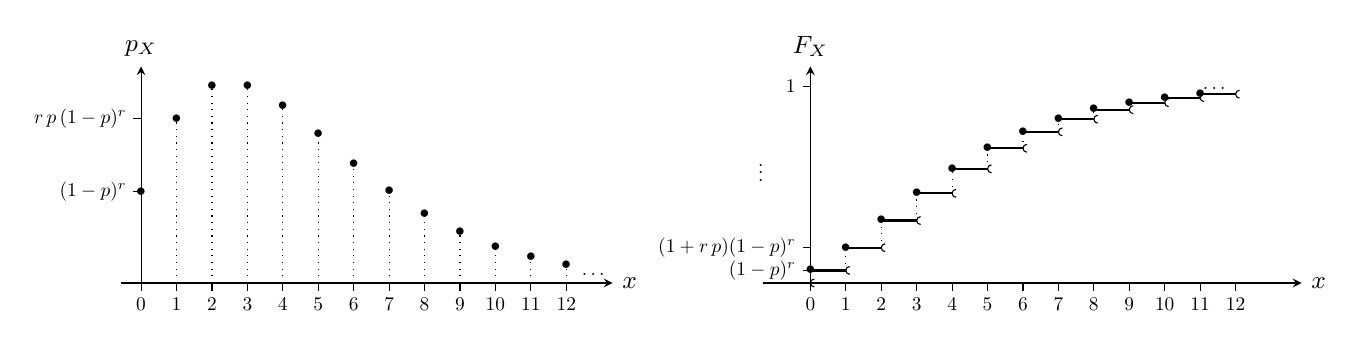
\begin{tikzpicture}%[scale=.9]
\shorthandoff{>}
%
\pgfmathsetmacro{\sx}{.45};% x-scaling
\pgfmathsetmacro{\r}{.05};% radius arc non continuity F_X
\pgfmathsetmacro{\p}{3/5};% probabilidad p de suceso
\pgfmathsetmacro{\rp}{3};% numero r de fracascos
\pgfmathsetmacro{\n}{12};% numero maximo a dibujar
\pgfmathsetmacro{\q}{max(floor((\rp-1)*\p/(1-\p)),0)};% modo de la binomial negativa
\pgfmathsetmacro{\m}{factorial(\q+\rp-1)*((1-\p)^\rp)*(\p^\q)/factorial(\rp-1)/factorial(\q)};
%{factorial(\n)/factorial(\q)/factorial(\n-\q)*(\p^\q)*((1-\p)^(\n-\q))};% maximo de la binomial
% masa
\begin{scope}
%
\pgfmathsetmacro{\sy}{2.5/\m};% y-scaling 
\draw[>=stealth,->] (-.25,0)--({\sx*(\n+.75)+.25},0) node[right]{\small $x$};
\draw[>=stealth,->] (0,-.1)--(0,{\sy*\m+.25}) node[above]{\small $p_X$};
%
\pgfmathsetmacro{\b}{(1-\p)^\rp};% coeficiente binomial por la probabilidad
%
\foreach \k in {0,...,\n} {
\draw ({\k*\sx},0)--({\k*\sx},-.1) node[below,scale=.7]{$\k$};
\draw[dotted] ({\k*\sx},0)--({\k*\sx},{\sy*\b}) node[scale=.7]{$\bullet$};
%
\pgfmathsetmacro{\bl}{\b*\p*(\k+\rp)/(\k+1)};\global\let\b\bl;% proba actualizada
}
\draw ({(\n+.25)*\sx},{\sy*\b*(\n+1)/\p/(\n+\rp)/2}) node[right,scale=.7]{\ldots};
\draw (0,{((1-\p)^\rp)*\sy})--(-.1,{((1-\p)^\rp)*\sy}) node[left,scale=.7]{$(1-p)^r$};
\draw (0,{\rp*\p*((1-\p)^\rp)*\sy})--(-.1,{\rp*\p*((1-\p)^\rp)*\sy}) node[left,scale=.7]{$r \, p \, (1-p)^r$};
%\draw (0,{(\rp*\p*((1-\p)^\rp)+\m)/2*\sy}) node[scale=.7]{$r \, p \, (1-p)^r$};
%
\end{scope}
%
%
% reparticion
\begin{scope}[xshift=8.5cm]
%
\pgfmathsetmacro{\sy}{2.5};% y-scaling 
%
\draw[>=stealth,->] (-.6,0)--({\sx*(\n+.75)+.5},0) node[right]{\small $x$};
\draw[>=stealth,->] (0,-.1)--(0,{\sy+.25}) node[above]{\small $F_X$};
%
\pgfmathsetmacro{\b}{(1-\p)^\rp};% coeficiente binomial por la probabilidad
\pgfmathsetmacro{\c}{(1-\p)^\rp};% cumulativa binomial por la probabilidad
%
% cumulativa x < 0
\draw (0,0)--(0,-.1) node[below,scale=.7]{$0$};
\draw[thick] (-.5,0)--(0,0);
\draw (\r,\r) arc (90:270:\r);
%
% cumulativa x de 0 a n-1
\foreach \k in {1,...,\n} {
\draw ({\k*\sx},0)--({\k*\sx},-.1) node[below,scale=.7]{$\k$};
\draw[thick]({(\k-1)*\sx},{\sy*\c}) node[scale=.7]{$\bullet$}--({\k*\sx},{\sy*\c});
\draw ({\k*\sx+\r},{\sy*\c+\r}) arc (90:270:\r);
\draw[dotted] ({(\k-1)*\sx},{(\c-\b)*\sy})--({(\k-1)*\sx},{\c*\sy});
%
\pgfmathsetmacro{\bl}{\b*\p*(\k+\rp-1)/\k};\global\let\b\bl;% proba actualizada
\pgfmathsetmacro{\cl}{\c+\b};\global\let\c\cl;% cumulativa actualizada
}
%
\draw ({\n*\sx},{\sy*(\c+1)/2}) node[left,scale=.7]{\ldots};
\draw (0,{((1-\p)^\rp)*\sy})--(-.1,{((1-\p)^\rp)*\sy}) node[left,scale=.7]{$(1-p)^r$};
\draw (0,{(1+\rp*\p)*((1-\p)^\rp)*\sy})--(-.1,{(1+\rp*\p)*((1-\p)^\rp)*\sy}) node[left,scale=.7]{$(1+r \, p) (1-p)^r$};
\draw (-.75,{((1+\rp*\p)*((1-\p)^\rp)+1)/2*\sy}) node[right,scale=.7]{$\vdots$};
\draw (0,\sy)--(-.1,\sy) node[left,scale=.7]{$1$};
\end{scope}
%
\end{tikzpicture} \end{center}
%
\leyenda{Ilustraci\'on de  una distribuci\'on de  probabilidad binomial negativa
  (a), y  la funci\'on  de repartici\'on  asociada (b), con  $r =  3, \quad  p =
  \frac35$.}
\label{Fig:MP:BinomialNegativa}
\end{figure}
\SZ{Otros ilustraciones para otros $r, p$?}

Esta ley aparece  cuando se repite una experencia  binaria \ $X_i \in \{  0 \; 1
\}, i  = 1,  \ldots$ \ con  \ $P(X_i=1)  = p$ \  de manera  independiente ($X_i$
independientes)  hasta que  \ $r$  \ variables  valen 0,  con \  $r$ \  fijo. El
n\'umero  de  excito  \ $X$  \  sigue  una  ley  \  $\B_-(r,p)$ (el  calculo  es
directo). Dicho de  otra manera, $X =  \sum_{i=1}^N X_i$ \ con \  $N$ \ variable
aleatoria tal que $X_N = 0$ \ y \ $r = \sum_{i=1}^N (1-X_i)$: condicionalmente a
\ $N$,  la variable \modif{\ $X$ } \  es binomial de parametro  $p$\modif{, \ie \
    $P(X=x|N=n) = \bino{n}{x} p^x (1-p)^{n-x}$}.  Se puede ver que \ $P(N = n) =
  \bino{n}{r-1} (1-p)^r p^{n-r}$ \ y la ley de la binomial negativa se recupera
\modif{a        trav\'es        del        teorema        de        probabilidad
  total~\ref{Teo:MP:ProbaTotalDiscreto}    o   tambi\'en,}   a    trav\'es   del
teorema~\ref{Teo:MP:SumaAleatoriaGeneradoraProbabilidad}.
%
% Blaise PAscal - Polya caso r real

Esta distribuci\'on se  generaliza para \ $r \in \Rset_+^*$ \  pero se pierde la
interpretaci\'on que v\'imos en el p\'arafo anterior.

Nota: cuando \ $p = 0$ \ la variable es cierta \ $X = r$.


% --------------------------------- Multinomial
\subsubseccion{Ley Multinomial}
\label{Sssec:MP:Multinomial}

Esta ley es una generalizaci\'on de la ley binomial y aparece por ejemplo cuando
se  repite  una  experiencia  a  \  $k$  \ estados  \  $n$  \  veces  de  manera
independiente y nos  interesamos a la probabilidad que  el primer evento aparece
$n_1$ veces,  el secundo  $n_2$ veces, \ldots  (ej. para  $k = 6$,  contamos los
n\'umeros de $1$, de $2$, \ldots cuando tiramos $n$ veces este dado).  Se denota
\ $X \ \sim \ \M(n,p)$ \ con \  $n \in \Nset^*$ \ y \ $p = \begin{bmatrix} p_1 &
  \cdots & p_k \end{bmatrix}^t \in  \Simp{k-1}$ \ the \ $(k-1)$-simplex estandar
(ver figure~\ref{Fig:MP:Dirichlet}-(a) y notaciones).   Entonces, a pesar de que
se escribe \  $X$ \ de manera $k$-dimensional, el vector  partenece a un espacio
claramente \ $d = k-1$ \ dimensional y en el caso \ $k = 2$ \ se recupera la ley
binomial.  Las caracter\'isticas de \ $X \ \sim \ \M(n,p)$ \ son las siguientes:

\begin{caracteristicas}
%
Dominio de definici\'on~\footnote{De hecho, se puede considerar que el vector
aleatorio es \ $(k-1)$-dimensional \ $\widetilde{X} = \begin{bmatrix}
\widetilde{X}_1 & \cdots & \widetilde{X}_{k-1} \end{bmatrix}^t$ \ definido sobre
el dominio \ $\widetilde{\X} = \left\{ x \in \{ 0 \; \ldots \; n\}^{k-1}, \:
\sum_{i=1}^{k-1} x_i \le n \right\}$.\label{Foot:MP:MultinomialDominio}} & $\X =
\left\{ x \in \{ 0 \; \ldots \; n\}^k \tq \sum_{i=1}^k x_i = n \right\}$\\[2mm]
\hline
%
Parametros~\footnote{El par\'ametro de \ $\widetilde{X}$ \ es \ $\widetilde{p} =
\protect\begin{bmatrix} p_1 & \cdots & p_{k-1} \end{bmatrix}^t\protect \in
\left\{ q \in [0 \; 1]^{k-1} \tq \sum_{i=1}^{k-1} q_i \le 1
\right\}$.\label{Foot:MP:MultinomialParametro}} & $n \in \Nset^*$, \quad $p \in
\Simp{k-1}$\\[2mm]
\hline
%
Distribuci\'on de probabilidad~\footnote{La masa de probabilidad de \
$\widetilde{X}$ \ es \ $p_{\widetilde{X}}(x) = \frac{n!}{\prod_{i=1}^{k-1} x_i!
(n-\sum_{i=1}^{k-1} x_i)!}  \prod_{i=1}^{k-1} p_i^{x_i} \, \left( 1 -
\sum_{i=1}^{k-1} p_i \right)^{n-\sum_{i=1}^{k-1}
x_i}$.\label{Foot:MP:MultinomialMasa}} & $\displaystyle p_X(x) =
\frac{n!}{\prod_{i=1}^k x_i!}  \prod_{i=1}^k p_i^{x_i}$\\[2mm]
\hline
%
Promedio & $\displaystyle m_X = n \, p$\\[2mm]
\hline
%
Covarianza~\footnote{$\Sigma_X \in P_k(\Rset)$, pero de \ $\un^t \Sigma_X \un =
0$ \ viene \ $\Sigma_X \not\in P_k^+(\Rset)$. Eso es la consecuencia directa del
hecho de que \ $X$ \ $d$-dimensional, vive sobre \ $\Simp{k-1}$,
$(d-1)$-dimensional.\label{Foot:MP::MultinomialCovarianza}} & $\displaystyle
\Sigma_X = n \left( \diag p - p \, p^t \right)$\\[2mm]
\hline
%
Generadora de probabilidad~\footnote{Notar: $G_{\widetilde{X}}\left(
\widetilde{z} \right) = G_X\left( \begin{bmatrix} \widetilde{z} &
1 \end{bmatrix}^t \right)$ \ y al rev\'es \ $G_X(z) = z_k^n \,
G_{\widetilde{X}}\left( \begin{bmatrix} \frac{z_1}{z_k} & \cdots &
\frac{z_{k-1}}{z_k} \end{bmatrix}^t
\right)$.\label{Foot:MP:MultinomialGeneProba}} & $\displaystyle G_X(z) = \left(
p^t z \right)^n$ \ para \ $z \in \Cset^k$\\[2mm]
\hline
%
Generadora de momentos~\footnote{Notar: $M_{\widetilde{X}}\left( \widetilde{u}
\right) = M_X\left( \begin{bmatrix} \widetilde{u} & 0 \end{bmatrix}^t \right)$ \
y \ $M_X(u) = e^{n \, u_k} M_{\widetilde{X}}\left( \begin{bmatrix} u_1 - u_k &
\cdots & u_{k-1} - u_k \end{bmatrix}^t
\right)$.\label{Foot:MP:MultinomialGeneMomentos}} & \protect$\displaystyle
M_X(u) = \left( p^t e^u \right)^n, \: e^u = \begin{bmatrix} e^{u_1} & \cdots &
e^{u_k} \end{bmatrix}^t$\protect \ para \ $u \in \Cset^k$\\[2mm]
\hline
%
Funci\'on caracter\'istica~\footnote{Notar: $\Phi_{\widetilde{X}}\left(
\widetilde{\omega} \right) = \Phi_X\left( \begin{bmatrix} \widetilde{\omega} &
0 \end{bmatrix}^t \right)$ \ o \ $\Phi_X(\omega) = e^{\imath \, n \, \omega_k}
\Phi_{\widetilde{X}}\left( \begin{bmatrix} \omega_1 - \omega_k & \cdots &
\omega_{k-1} - \omega_k \end{bmatrix}^t
\right)$.\label{Foot:MP:MultinomialCaracteristica}} & $\displaystyle
\Phi_X(\omega) = \left( p^t e^{\imath \omega} \right)^n$
\end{caracteristicas}

% Momentos & $ \Esp\left[ X^k \right] = ??\\[2mm]
% Momento factorial & $\Esp\left[ (X)_k \right] = 
% \frac{(r+k-1)!}{(r-1)!} \left( \frac{p}{1-p} \right)^k$\\[2mm]
% Modo $\left\lfloor (n+1) p \right\rfloor$
% Mediana $\left\lfloor n p \right\rfloor$ o $\left\lceil n p \right\rceil
% CDF	$I_{1-p}(n-k,k+1)$ regularized incomplete beta function

Su masa  de probabilidad  y funci\'on de  repartici\'on son representadas  en la
figura Fig.~\ref{Fig:MP:Multinomial}.
%
\begin{figure}[h!]
\begin{center} 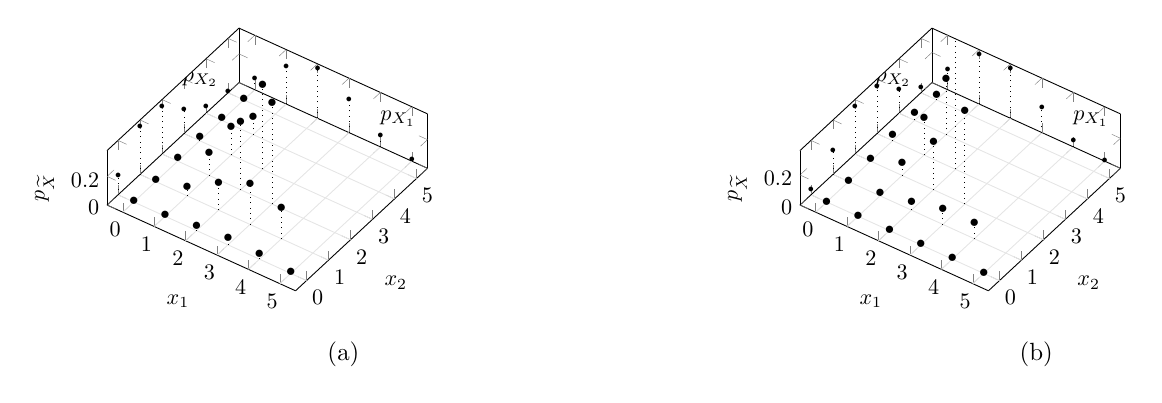
\begin{tikzpicture}[scale=.8]
\shorthandoff{>}
%
%
\pgfmathsetmacro{\n}{5};% numeros para la multinomial
\pgfmathsetmacro{\dec}{.5};% shitf para dibujar las marginales
%
% Ejemplo [6 5 4]/15
\begin{scope}
%
\pgfmathsetmacro{\pu}{2/5};% p_1
\pgfmathsetmacro{\pd}{1/3};% p_2
\pgfmathsetmacro{\qu}{floor((\n+1)*\pu)};% modo de la binomial 1
\pgfmathsetmacro{\qd}{floor((\n+1)*\pd)};% modo de la binomial 2
\pgfmathsetmacro{\mau}{factorial(\n)/factorial(\qu)/factorial(\n-\qu)*(\pu^\qu)*((1-\pu)^(\n-\qu))};% maximo de la binomial 1
\pgfmathsetmacro{\mad}{factorial(\n)/factorial(\qd)/factorial(\n-\qd)*(\pd^\qd)*((1-\pd)^(\n-\qd))};% maximo de la binomial 2
\pgfmathsetmacro{\ma}{max(\mau,\mad)};% maximo de ambas binomiales
%
\begin{axis}[
    colormap = {whiteblack}{color(0cm)  = (white);color(1cm) = (black)},
    width=.55\textwidth,
    view={35}{70},
    enlargelimits=false,
    xmin={-\dec},
    xmax={\n+\dec},
    ymin={-\dec},
    ymax={\n+\dec},
    zmax={1.1*\ma},
    color=black,
    xtick={0,...,\n},
    ytick={0,...,\n},
    xlabel=$x_1$,
    ylabel=$x_2$,
    zlabel=$p_{\widetilde{X}}$,
]
%
% Lineas
\foreach \mu in {0,...,\n} {
  %
  % lineas (m1,m2) abajo
  \addplot3 [domain={-\dec}:{\n+\dec},samples=2, samples y=0,color=black!10] (\mu,\x,0);
  \addplot3 [domain={-\dec}:{\n+\dec},samples=2, samples y=0,color=black!10] (\x,\mu,0);
}
%
\pgfmathsetmacro{\bu}{(1-\pu-\pd)^\n};% coeficiente binomial por la probabilidad p1
\pgfmathsetmacro{\bd}{\bu};% coeficiente binomial por la probabilidad p2
%
\pgfmathsetmacro{\bmu}{(1-\pu)^\n};% lo mismo para la marginale 1
\pgfmathsetmacro{\bmd}{(1-\pd)^\n};% lo mismo para la marginale 2
%
\foreach \mu in {0,...,\n} {
  \foreach \md in {0,...,\n} {
    \ifnum \numexpr\mu+\md < \numexpr\n+1
      \addplot3 [dotted,domain=0:\bd,samples=2, samples y=0,color=black]
      (\mu,\md,\x)  node[scale=.85]{$\bullet$};
      %
      \pgfmathsetmacro{\bld}{\bd*\pd*(\n-\md)/((\md+1)*(1-\pu-\pd))};
      \global\let\bd\bld;% proba en m2 (m1 fijo) actualizado
    \fi
  }
  %
  % Marginales
  \addplot3 [dotted,domain=0:\bmu,samples=2, samples y=0,color=black]
  (\mu,{\n+\dec},\x)  node[scale=.55]{$\bullet$};
  \addplot3 [dotted,domain=0:\bmd,samples=2, samples y=0,color=black]
  ({-\dec},\mu,\x)  node[scale=.55]{$\bullet$};
  %
  \pgfmathsetmacro{\blu}{\bu*\pu*(\n-\mu)/((\mu+1)*(1-\pu-\pd))};
  \global\let\bu\blu;\global\let\bd\blu;% proba inicial en m1 actualizada
  %
  % lo mismo para cada marginal
  \pgfmathsetmacro{\blmu}{\bmu*\pu*(\n-\mu)/((\mu+1)*(1-\pu))};
  \global\let\bmu\blmu;% proba 1 actualizada
  \pgfmathsetmacro{\blmd}{\bmd*\pd*(\n-\mu)/((\mu+1)*(1-\pd))};
  \global\let\bmd\blmd;% proba 2 actualizada
}
%
\node at (axis cs:{3*\n/4},{\n+\dec},{\mau/2})[right]{$p_{X_1}$};
\node at (axis cs:{-\dec},{3*\n/4},{\mad/2})[above]{$p_{X_2}$};
%
\end{axis}
\node at ({3*\n/4},-1)[scale=.9]{(a)};
\end{scope}
%
%
% Ejemplo [1 1 1]/3
\begin{scope}[xshift = 11cm]
%
\pgfmathsetmacro{\pu}{1/3};% p_1
\pgfmathsetmacro{\pd}{1/2};% p_2
\pgfmathsetmacro{\qu}{floor((\n+1)*\pu)};% modo de la binomial 1
\pgfmathsetmacro{\qd}{floor((\n+1)*\pd)};% modo de la binomial 2
\pgfmathsetmacro{\mau}{factorial(\n)/factorial(\qu)/factorial(\n-\qu)*(\pu^\qu)*((1-\pu)^(\n-\qu))};% maximo de la binomial 1
\pgfmathsetmacro{\mad}{factorial(\n)/factorial(\qd)/factorial(\n-\qd)*(\pd^\qd)*((1-\pd)^(\n-\qd))};% maximo de la binomial 2
\pgfmathsetmacro{\ma}{max(\mau,\mad)};% maximo de ambas binomiales
%
\begin{axis}[
    colormap = {whiteblack}{color(0cm)  = (white);color(1cm) = (black)},
    width=.55\textwidth,
    view={35}{70},
    enlargelimits=false,
    xmin={-\dec},
    xmax={\n+\dec},
    ymin={-\dec},
    ymax={\n+\dec},
    zmax={1.1*\ma},
    color=black,
    xtick={0,...,\n},
    ytick={0,...,\n},
    xlabel=$x_1$,
    ylabel=$x_2$,
    zlabel=$p_{\widetilde{X}}$,
]
%
% Lineas
\foreach \mu in {0,...,\n} {
  %
  % lineas (m1,m2) abajo
  \addplot3 [domain={-\dec}:{\n+\dec},samples=2, samples y=0,color=black!10] (\mu,\x,0);
  \addplot3 [domain={-\dec}:{\n+\dec},samples=2, samples y=0,color=black!10] (\x,\mu,0);
}
%
\pgfmathsetmacro{\bu}{(1-\pu-\pd)^\n};% coeficiente binomial por la probabilidad p1
\pgfmathsetmacro{\bd}{\bu};% coeficiente binomial por la probabilidad p2
%
\pgfmathsetmacro{\bmu}{(1-\pu)^\n};% lo mismo para la marginale 1
\pgfmathsetmacro{\bmd}{(1-\pd)^\n};% lo mismo para la marginale 2
%
\foreach \mu in {0,...,\n} {
  \foreach \md in {0,...,\n} {
    \ifnum \numexpr\mu+\md < \numexpr\n+1
      \addplot3 [dotted,domain=0:\bd,samples=2, samples y=0,color=black]
      (\mu,\md,\x)  node[scale=.85]{$\bullet$};
      %
      \pgfmathsetmacro{\bld}{\bd*\pd*(\n-\md)/((\md+1)*(1-\pu-\pd))};
      \global\let\bd\bld;% proba en m2 (m1 fijo) actualizado
    \fi
  }
  %
  % Marginales
  \addplot3 [dotted,domain=0:\bmu,samples=2, samples y=0,color=black]
  (\mu,{\n+\dec},\x)  node[scale=.55]{$\bullet$};
  \addplot3 [dotted,domain=0:\bmd,samples=2, samples y=0,color=black]
  ({-\dec},\mu,\x)  node[scale=.55]{$\bullet$};
  %
  \pgfmathsetmacro{\blu}{\bu*\pu*(\n-\mu)/((\mu+1)*(1-\pu-\pd))};
  \global\let\bu\blu;\global\let\bd\blu;% proba inicial en m1 actualizada
  %
  % lo mismo para cada marginal
  \pgfmathsetmacro{\blmu}{\bmu*\pu*(\n-\mu)/((\mu+1)*(1-\pu))};
  \global\let\bmu\blmu;% proba 1 actualizada
  \pgfmathsetmacro{\blmd}{\bmd*\pd*(\n-\mu)/((\mu+1)*(1-\pd))};
  \global\let\bmd\blmd;% proba 2 actualizada
}
%
\node at (axis cs:{3*\n/4},{\n+\dec},{\mau/2})[right]{$p_{X_1}$};
\node at (axis cs:{-\dec},{3*\n/4},{\mad/2})[above]{$p_{X_2}$};
\end{axis}
\node at ({3*\n/4},-1)[scale=.9]{(b)};
\end{scope}
%
\end{tikzpicture} \end{center}
%
\leyenda{Ilustraci\'on de una distribuci\'on  de probabilidad multinomial para \
  $k   =  3$   \   del   vector  \   $(k-1)$-dimensional   \  $\widetilde{X}   =
  \protect\begin{bmatrix}   X_1  &  X_2   \protect\end{bmatrix}^t$  \   ($X_3  =
  1-X_1-X_2$)  \ con  las marginales  \ $p_{X_1},  \: p_{X_2}$  \ (ver  notas de
  pie~\ref{Foot:MP:MultinomialDominio}   y~\ref{Foot:MP:MultinomialMasa}).    Es
  dibujada solamente  la distribuci\'on sobre  $\X$, siendo esta nula  afuera de
  $\X$.  Los parametros son \ $n = 5$ \ y \ $p = \protect\begin{bmatrix} \frac25
    &    \frac13    &   \frac4{15}    \protect\end{bmatrix}^t$    (a),   $p    =
  \protect\begin{bmatrix} \frac13  & \frac12 &  \frac16 \protect\end{bmatrix}^t$
  (b).}
\label{Fig:MP:Multinomial}
\end{figure}


Notar: cuando $p = \un_i$, la variable es cierta $X = n \un_i$.

\SZ{Otros ilustraciones para otros $n, p$?}


Vectores  de  distribuci\'on  multinomial  tienen  una  propiedade  notable  con
respecto a una permutaci\'on de variable, parecidas a la de la binomial:
%
\begin{lema}[Efecto de una permutaci\'on]\label{Lem:MP:PermutacionMultinomial}
%
  Sea \ $X \, \sim \, \M(n,p), \: p \in \Simp{k-1}$ \ y \ $\Pi \in \perm_k(\Rset)$ \
  matriz \ de permutaci\'on. Entonces
  %
  \[
  \Pi X \, \sim \, \M\left( n ,  \Pi p \right)
  \]
  %
\end{lema}
%
\begin{proof}
  El  resultado  es  inmediato  saliendo  de  la  funci\'on  caracter\'istica  y
  aplicando  el  teorema~\ref{Teo:MP:PropiedadesFuncionCaracteristica} (recordar
  que $\Pi^{-1} = \Pi^t$). M\'as directamente, notando la permutation \ $\sigma$
  \ tal que  \ $\Pi = \sum_{i=1}^k \un_i \un_{\sigma(i)}^t$, se  puede ver que \
  $\displaystyle  P(\Pi X =  x) =  P(X =  \Pi^{-1} x)  = \frac{n!}{\prod_{i=1}^k
    x_{\sigma^{-1}(i)}!}       \prod_{i=1}^k      p_i^{x_{\sigma^{-1}(i)}}     =
  \frac{n!}{\prod_{i=1}^k x_i!}  \prod_{i=1}^k p_{\sigma(i)}^{x_i}$ \ por cambio
  de indices.
\end{proof}
%
Adem\'as ley  multinomial exhibe una stabilidad remplazando  dos componentes por
su suma:
%
\begin{lema}[Stabilidad por agregaci\'on]\label{Lem:MP:StabAgregacionMultinomial}
%
  Sea  \ $X =  \begin{bmatrix} X_1  & \cdots  & X_k  \end{bmatrix}^t \,  \sim \,
  \M(n,p), \:  p \in \Simp{k-1}$ \ y  \ $G^{(i,j)}$ \ matriz  de agrupaci\'on de
  las $(i,j)$-\'esima componentes (ver notaciones). Entonces,
  %
  \[
  G^{(i,j)} X \, \sim \, \M\left( n , G^{(i,j)} p \right)  
  \]
  %
\end{lema}
%
Este resultado es  intuitivo en el hecho  de que vuelve a agrupar  los estados \
$i$ \ e \ $j$ \ en un estado, que tiene entonces la probabilidad \ $p_i + p_j$ \
de aparecer.
%
\begin{proof}
  Suponemos $i <  j$ (el otro caso  se recupera por simetr\'ia). A  partir de la
  funci\'on                 caracter\'istica                 y                el
  teorema~\ref{Teo:MP:PropiedadesFuncionCaracteristica} se tiene,
  %
  \begin{eqnarray*}
  \forall \: \omega \in \Rset^{k-1}, \quad \Phi_{G^{(i,j)} X}(\omega) & = &
  \Phi_X\left( G^{(i,j) \, t} \omega \right)\\[2mm]
  %
  & = & \left( \sum_{l=1}^k p_l \, e^{\imath \, \left( G^{(i,j) \, t} \omega \right)_l } \right)^n
  \end{eqnarray*}
  %
  Ahora,  se nota  que \  $G^{(i,j) \,  t} \omega  = \begin{bmatrix}  \omega_1 &
    \cdots    &   \omega_{j-1}   &    \omega_i   &    \omega_{j+1}   &    \cdots   &
    \omega_{k-1} \end{bmatrix}^t$, entonces
  %
  \begin{eqnarray*}
  \forall \: \omega \in \Rset^{k-1}, \quad \Phi_{G^{(i,j)} X}(\omega) & = &
  \left( \sum_{l=1, l \ne j}^k p_l \, e^{\imath \, \omega_l} + p_j \, e^{\imath \,
  \omega_i } \right)^n\\[2mm]
  %
  & = & \left( \sum_{l=1, l \ne i, l \ne j}^k p_l \, e^{\imath \, \omega_l} +
  (p_i+p_j) \, e^{\imath \, \omega_i } \right)^n
  %
  \end{eqnarray*}
  %
  lo que  cierra la  prueba. Se puede  tener un  enfoque m\'as directo,  con los
  mismos         pasos        que         en        la         prueba        del
  lema~\ref{Lem:MP:StabAgregacionHipergeomMulti}    tratando     de    la    ley
  hipergeometrica multivaluada.
\end{proof}

De este lema, aplicado de manera recursiva, se obtiene los corolarios siguientes:
%
\begin{corolario}\label{Cor:MP:MarginalMultinomial}
%
  Sea  \ $X  \,  \sim \,  \M(n,p)$, entonces  \  $\displaystyle X_i  \, \sim  \,
  \B(n,p_i)$.
\end{corolario}


Al final, por una analisis  combinatorial, se muestra sencillamente un resultado
similar al de la binomial como suma de Bernoulli independientes:
%
\begin{lema}\label{Lem:MultinomialSumaMultiBernoulli}
%
  Sean \ $U_i, \quad i = 1, \ldots ,  n, \: j = 1, \ldots , n$ \ discretas sobre
  $\U  = \{  1 \;  \ldots \;  k \}$  de masa  de probabilidad  $p_{U_i} =  p \in
  \Delta_{k-1}$, independientes, y $X_i = \un_{U_i} \in \Rset^k$. Entonces
  %
  \[
  \sum_{i=1}^n X_i \, \sim \, \M(n,p)
  \]
\end{lema}


% --------------------------------- Hipergeometrica
\subsubseccion{Ley hipergeometrica}
\label{Sssec:MP:Hipergeometrica}

Esta ley aparece por ejemplo cuando  se hace una experiencia con una poblaci\'on
de tama\~no \  $n$ \ (ej.  $n$ bolas  en una urna), que pueden  partenecer a dos
clases, con  \ $k$ \ num\'ero  de elementos de  la primera clase (a  veces dicho
estados de excito; ej. $k$ \ bolas  negras), $n-k$ \ num\'ero de elementos de la
secunda clase, y se  hace \ $m$ \ tiros si reemplazamiento.   $X$ es el n\'umero
de  tiros parteneciendo  en la  primera clase  (n\'umero de  excitos).  Esta ley
apareci\'o en trabajos de de Moivre en 1710~\cite{Moi10, Hal90, DavEdw01}.

Se denota \ $X \, \sim \, \H(n,k,m)$ \  con \ $n \in \Nset^*$, \quad $k \in \{ 0
\;  \ldots  \;  n  \}$,  \quad  $m  \in  \{  0 \;  \ldots  \;  m  \}$  \  y  sus
caracter\'isticas son las siguientes:

\begin{caracteristicas}
%
Dominio de definici\'on & $\X = \left\{ \max(0,k+m-n) \; \ldots \; \min(k,m)
\right\}$\\[2mm]
\hline
%
Par\'ametros & $n \in \Nset^*$ \: (poblaci\'on)\newline $k \in \{ 0 \; \ldots \;
n\}$ \ (n\'umero de estados exitosos)\newline $m \in \{ 0 \; \ldots \; n\}$ \:
(n\'umero de tiros)\\[2mm]
\hline
%
Distribuci\'on de probabilidad & \protect$p_X(x) =
\frac{\smallbino{k}{x} \smallbino{n-k}{m-x}}{\smallbino{n}{m}}$\protect\\[2mm]
\hline
%
Promedio & $\displaystyle m_X = \frac{m}{n} \, k$\\[2mm]
\hline
%
Varianza~\footnote{En el caso degenerado \ $n = 1$, o \ $m = 0$, o \ $m = 1 =
n$; en ambos casos, la variable es cierta (ver fin de la
subsecci\'on).\label{Foot:MP:HipergeometricaVarianza}} & $\displaystyle
\sigma_X^2 = \left\{ \protect\begin{array}{ccc} \frac{m \, (n-m)}{n^2 (n-1)} \,
k \, (n-k) & \mbox{si} & n > 1\\[2mm] 0 & \mbox{si} & n =
1\end{array}\protect\right.$\\[2mm]
\hline
%%
%Sesgo~\footnote{Cuando \ $m \in \{ 0 \; n \}$, tenemos \ $k \in \{ 0 \; n
%\}$. Entonces, la variable es cierta (ver fin de la subsecci\'on) as\'i que no
%hay asimetr\'ia. Si \ $n = 2$, \ y \ $k=m=1 \not\in \{0 \; n \}$, tenemos $P(X =
%0) = P(X = 1) = \frac12$ sim\'etrico: de nuevo el sesgo vale cero.} &
%$\displaystyle \gamma_X = \left\{ \!\! \begin{array}{cl} \frac{(n - 2 k) (n - 2
%m)}{n-2} % \sqrt{\frac{n-1}{m k (n-k) (n-m)}} & \mbox{si} \: n \ne 2, \quad k,l
%\not\in \{ 0 \; n \} \\[2mm] 0 & \mbox{si no} \end{array} \right.$\\[2mm]
%\hline
%%
%Curtosis por exceso & $\displaystyle \widebar{\kappa}_X = $\\[2mm]
% 0 si no
%\hline
%
Generadora de probabilidad & $G_X(z) = \frac{\smallbino{n-k}{m}}{\smallbino{n}{m}} \:
\: \hypgeom{2}{1}(-m , -k ; n-m-k+1 ; z)$ \ sobre \ $\Cset$\\[2mm]
\hline
%
Generadora de momentos & $M_X(u) = \frac{\smallbino{n-k}{m}}{\smallbino{n}{k}}  \:
\: \hypgeom{2}{1}\left( -m , -k ; n-m-k+1 ; e^u \right)$ \ sobre \
$\Cset$\\[2mm]
\hline
%%
Funci\'on caracter\'istica  & $\Phi_X(\omega) =  \frac{\smallbino{n-k}{m}}{\smallbino{n}{m}}  \:
\: \hypgeom{2}{1}\left( -m , -k ; n-m-k+1 ; e^{\imath \, \omega} \right)$
\end{caracteristicas}

Su masa  de probabilidad  y funci\'on de  repartici\'on son representadas  en la
figura Fig.~\ref{Fig:MP:Hipergeometrica}.
%
\begin{figure}[h!]
\begin{center} \begin{tikzpicture}[fixed point arithmetic]%[scale=.9]
\shorthandoff{>}
%
\pgfmathsetmacro{\sx}{.375};% x-scaling
\pgfmathsetmacro{\r}{.05};% radius arc non continuity F_X
%\pgfmathsetmacro{\p}{1/3};% probabilidad p
\pgfmathsetmacro{\n}{100};% numero n de la poblacion
\pgfmathsetmacro{\k}{12};% numero k de estados exitosos
\pgfmathsetmacro{\m}{40};% numero m de tiros
%
% Nota : con el fixed point, no anda min & max
% pero max(a,b) = (a+b+abs(a-b))/2  & min(a,b) = (a+b-abs(a-b))/2;
\pgfmathsetmacro{\f}{(\k+\m-abs(\k-\m))/2}; % ultimo indice de proba non nula
\pgfmathsetmacro{\F}{(\k+\m+abs(\k-\m))/2}; %
\pgfmathsetmacro{\d}{(abs(\m-\n+\k)+\m-\n+\k)/2}; % primer indice de proba non nula
%
% ultima proba non nula F (F-1) ... (F-f+1) / n (n-1) ... (n-f+1)
% finhiper(\F,\n,\f)
\tikzmath{function finhiper(\a,\b,\c) {
    if \c == 1 then {return (\a/\b;}
    else {return (\a/\b)*finhiper(\a-1,\b-1,\c-1);};
};};
%

\pgfmathsetmacro{\dn}{\d-1}; % proba nula hasta d-1
\pgfmathsetmacro{\fn}{\f+1}; % proba nula de nuevo a partid de f-1
\pgfmathsetmacro{\ui}{\f+3}; % ultimo indice dibujado
% f, f-1... hasta d => y de 0 hasta f-d & x = f-y
\pgfmathsetmacro{\finy}{\f-\d}
%
% masa
\begin{scope}
%
\pgfmathsetmacro{\sy}{10};% y-scaling
%
% proba nulas del principio 0 -> d-1
\foreach \y in {-2,...,\dn} {
\pgfmathsetmacro{\xl}{int(\y)};\global\let\x\xl;
\draw ({\sx*\x},0)--({\sx*\x},-.1) node[below,scale=.7]{$\x$};
\draw ({\sx*\x},0) node[scale=.6]{$\bullet$};
}
%
% proba nulas del fin f+1 -> ui
\foreach \y in {\fn,...,\ui} {
\pgfmathsetmacro{\xl}{int(\y)};\global\let\x\xl;
\draw ({\sx*\x},0)--({\sx*\x},-.1) node[below,scale=.7]{$\x$};
\draw ({\sx*\x},0) node[scale=.6]{$\bullet$};
}
%
\pgfmathsetmacro{\pr}{finhiper(\F,\n,\f)};% valor del ultima proba no nula
\pgfmathsetmacro{\maxp}{\pr};% proba maximal (inicializacion)
%
\foreach \y in {0,...,\finy} {
\pgfmathsetmacro{\xl}{int(\f-\y)};\global\let\x\xl;
\draw ({\sx*\x},0)--({\sx*\x},-.1) node[below,scale=.7]{$\x$};
\draw[dotted] ({\sx*\x},0)--({\sx*\x},{\sy*\pr}) node[scale=.6]{$\bullet$};
%
\pgfmathsetmacro{\prl}{\pr*\x*(\n-\k-\m+\x)/((\m-\x+1)*(\k-\x+1))};\global\let\pr\prl;% proba actualizado
\pgfmathsetmacro{\maxpl}{(abs(\pr-\maxp)+\pr+\maxp)/2};\global\let\maxp\maxpl;% proba max actualizado
}
%
\draw[>=stealth,->] ({-2*\sx-.25},0)--({\sx*\ui+.35},0) node[right]{\small $x$};
\draw[>=stealth,->] (0,-.15)--(0,{\sy*\maxp+.25}) node[above]{\small $p_X$};
%\draw (0,{((1-\p)^\n)*\sy})--(-.1,{((1-\p)^\n)*\sy}) node[left,scale=.7]{$(1-p)^n$};
%\draw (0,{\n*\p*((1-\p)^(\n-1))*\sy})--(-.1,{\n*\p*((1-\p)^(\n-1))*\sy}) node[left,scale=.7]{$n \, p \, (1-p)^{n-1}$};
%
\node at ({(\sx*(2+\f)+.25)/2},-1) [scale=.9]{(a)};
\end{scope}
%
%
% reparticion
\begin{scope}[xshift=8.25cm]
%
\pgfmathsetmacro{\sy}{2.5};% y-scaling 
%
\draw[>=stealth,->] ({-2*\sx-.25},0)--({\sx*\ui+.5},0) node[right]{\small $x$};
\draw[>=stealth,->] (0,-.15)--(0,{\sy+.25}) node[above]{\small $F_X$};
%
% proba nulas del principio 0 -> d-1
\foreach \y in {-2,...,\dn} {
\pgfmathsetmacro{\xl}{int(\y)};\global\let\x\xl;
\draw ({\sx*\x},0)--({\sx*\x},-.1) node[below,scale=.7]{$\x$};
}
\draw ({-2*\sx},0)--({\sx*\d},0);
%
% proba nulas del fin f+1 -> ui
\foreach \y in {\fn,...,\ui} {
\pgfmathsetmacro{\xl}{int(\y)};\global\let\x\xl;
\draw ({\sx*\x},0)--({\sx*\x},-.1) node[below,scale=.7]{$\x$};
}
\draw ({\sx*\ui},\sy)--({\sx*(\f+1)},\sy);
%
\pgfmathsetmacro{\pr}{finhiper(\F,\n,\f)};% valor del ultima proba no nula
\pgfmathsetmacro{\cum}{1};% valor final de la cumulativa
% f, f-1... hasta d => y de 0 hasta f-d & x = f-y
\foreach \y in {0,...,\finy} {
\pgfmathsetmacro{\xl}{int(\f-\y)};\global\let\x\xl;
\draw ({\sx*\x},0)--({\sx*\x},-.1) node[below,scale=.7]{$\x$};
\draw ({\sx*(\x+1)},{\sy*\cum})--({\sx*\x},{\sy*\cum}) node[scale=.6]{$\bullet$};
\draw ({\sx*\x+\r},{\sy*(\cum-\pr)+\r}) arc (90:270:\r);
\draw[dotted] ({\sx*\x},{\sy*\cum})--({\sx*\x},{\sy*(\cum-\pr)});
%
\pgfmathsetmacro{\cuml}{\cum-\pr}\global\let\cum\cuml;% cumulativa actualizada
\pgfmathsetmacro{\prl}{\pr*\x*(\n-\k-\m+\x)/((\m-\x+1)*(\k-\x+1))};\global\let\pr\prl;% proba actualizado
}
%\draw (0,{((1-\p)^\n)*\sy})--(-.1,{((1-\p)^\n)*\sy}) node[left,scale=.7]{$(1-p)^n$};
%\draw (0,{\n*\p*((1-\p)^(\n-1))*\sy})--(-.1,{\n*\p*((1-\p)^(\n-1))*\sy}) node[left,scale=.7]{$n \, p \, (1-p)^{n-1}$};
%
\node at ({(\sx*(\ui+2)+.5)/2},-1) [scale=.9]{(b)};
\end{scope}
%
\end{tikzpicture} \end{center}
%
\leyenda{Ilustraci\'on  de una  distribuci\'on  de probabilidad  Hipergeometrica
  (a), y la funci\'on de repartici\'on asociada (b), con \ $n = 100$, \quad $k =
  12$, \quad $m = 40$.}
\label{Fig:MP:Hipergeometrica}
\end{figure}

\SZ{Otros ilustraciones para otros $n, k, m$?

  Poner el  Sesgo (ya  lo tengo)?  El Curtosis (lo  tengo que  simplificar)? muy
  pesadas...      Momento      factorial      $f_q      =      \frac{\PocD{m}{q}
    \PocD{k}{q}}{\PocD{n}{q}}$ permitiendo calcular todo.}

Notar: la variable resuelta cierta en los casos siguientes
%
\begin{itemize}
\item  $m = 0  \: \Rightarrow  \: X  = 0$:  no se  sortean elementos,  as\'i que
  siempre se sortea $0$ elementos de la primera clase;
%
\item $m =  n \: \Rightarrow \: X =  k$: si se sortean todos los  elementos de la
  poblaci\'on, se sortean todos los \ $k$ \ de la primera clase;
%
\item $k = 0 \: \Rightarrow \: X = 0$: si la primera clase no tiene elementos, no
  se puede tirar elementos de esta clase;
%
\item $k = n  \: \Rightarrow \: X = m$: al rev\'es si  la secunda clase no tiene
  elementos, todos los sorteados partenecen a la primera clase.
\end{itemize}

La ley tiene propiedades de reflexividad del mismo tipo que para la ley binomial:
%
\begin{lema}[Reflexividad]
\label{Lem:MP:ReflexividadHipergeometrica}
%
  Sea \ $X \, \sim \, \H(n,k,m)$. Entonces
  %
  \[
  m-X \, \sim \, \H(n,n-k,m) \qquad \mbox{y} \qquad k-X \sim \H(n,k,n-m)
  \]
  %
\end{lema}
%
Se puede ver  que si en una urna con  bolas negras y blancas, con  \ $k$ \ bolas
negras, y \ $X$  \ es el n\'umero de bolas negras  sorteadas, $m-X$ \ representa
las bolas blancas sorteadas. Es decir que  en \ $m-X$ \ se intercambia los roles
de las bolas  negras y blancas.  De la misma manera,  $k-X$ representa las bolas
negras que quedan en la urna, entre las  \ $n-m$ \ que quedan, es decir que en \
$k-X$ \ se intercambia  los roles de las bolas sorteadas y  las que quedan en la
urna. M\'as formalmente:
%
\begin{proof}
  El  primer   resultado  es  inmediato  de  $P(m-X   =  x)  =  P(X   =  m-x)  =
  \frac{\smallbino{k}{m-x} \smallbino{n-k}{x}}{\smallbino{n}{m}}$. El secundo de
  $P(k-X    =     x)    =     P(X    =    k-x)     =    \frac{\smallbino{k}{k-x}
    \smallbino{n-k}{m-k+x}}{\smallbino{n}{m}}      =      \frac{\smallbino{k}{x}
    \smallbino{n-k}{n-m-x}}{\smallbino{n}{n-m}}$  notando   que  $\bino{a}{b}  =
  \bino{a}{a-b}$.
\end{proof}

% Cuando  $n  = 1$,  se  recupera  la lei  de  Bernoulli  $\B(p) \equiv  \B(1,p)$.
% Ad\'emas, se muestra  sencillamente usando la generadora de  probabilidad que
% %
% De este resultado,  se puede notar que, por  ejemplo, le distribuci\'on binomial
% aparece en el conteo de eventos independientes de misma probabilidad entre $n$.

% Tambi\'en,  la ley binomial  tiene una  propiedad de  reflexividad, consecuencia
% directa de la de Bernoulli:
% %
% \begin{lema}[Reflexividad]
% \label{Lem:MP:ReflexividadBinomial}
% %
%   Sea \ $X \, \sim \, \B(n,p)$. Entonces
%   %
%   \[
%   n-X \, \sim \, \B(n,1-p)
%   \]
%   %
% \end{lema}

% Nota que cuando $p = 0$ (resp. $p = 1$) la variable es cierta $X = 0$ (resp.  $X
% = n$).



% --------------------------------- Hipergeometrica Negativa
\subsubseccion{Ley hipergeometrica Negativa}
\label{Sssec:MP:HipergeometricaNegativa}

Esta ley aparece  por ejemplo cuando se hace una experiencia  del mismo tipo que
para la hipergeometrica, con una poblaci\'on de tama\~no \ $n$ \ (ej.  $n$ bolas
en  una urna),  que pueden  partenecer a  dos clases,  con \  $k$ \  num\'ero de
elementos de la primera clase estados  de excito; ej. $k$ \ bolas negras), $n-k$
\ num\'ero  de elementos de la  secunda clase.  Pero en  lugar de hacer  \ $m$ \
tiros  fijos,  se  hace tiros  hasta  que  $r$  elementos  de la  seconda  clase
(fracascos)  sean tiradas.   $X$ es  el n\'umero  de tiros  parteneciendo  en la
primera clase  (n\'umero de excitos). Es decir  que cuando $X =  x$, tenemos $k$
elementos de  la primera clase en  los ``primeros'' $x+r-1$  tiros, el \'ultimos
parteneciendo a la seconda clase.  Parece que se encuentran las primeras huellas
de esta ley en trabajos del marquesano de Condorcet en 1785~\cite{Con85}.

Se denota \ $X \,  \sim \, \H_-(n,k,r)$ \ con \ $n \in \Nset^*$,  \quad $k \in \{ 0 \;
\ldots \; n \}$, \quad $m \in \{  0 \; \ldots \; n-k \}$ \ y sus caracter\'isticas
son las siguientes:

\begin{caracteristicas}
%
Dominio de definici\'on & $\X = \left\{ 0 \; \ldots \; k \right\}$\\[2mm]
\hline
%
Parametros & $n \in \Nset^*$ \: (poblaci\'on)\newline $k \in \{ 0 \; \ldots \;
n\}$ \ (n\'umero de estados exitosos)\newline $r \in \{ 0 \; \ldots \; n-k\}$ \:
(n\'umero de fracascos para parar)\\[2mm]
\hline
%
Distribuci\'on de probabilidad~\footnote{Para los $x+r-1$ primeros tiros, de la
primera clase hay $\smallbino{k}{x}$ combinaciones posibles, y
$\smallbino{n-k}{r-1}$ de la seconda clase, sobre los $\smallbino{n}{x+r-1}$
combinaciones posibles en total. Para el \'ultimo tiro, quedan $n-k-(r-1)$
posibilidades de la seconda clase sobre las $n-x-(r-1)$ elementos que quedan.} &
\protect$p_X(x) = \left\{ \begin{array}{ccc} \frac{\smallbino{x+r-1}{x}
\smallbino{n-r-x}{k-x}}{\smallbino{n}{k}} & \mbox{si} & r > 0\\ \un_{\{0\}}(x) & \mbox{si} & r = 0 \end{array} \right.$\protect\\[2mm]
\hline
%
Promedio & $\displaystyle m_X = \frac{r \, k}{n - k + 1}$\\[2mm]
\hline
%
Varianza & $\displaystyle \sigma_X^2 = \frac{r \, k (n+1) (n-k-r+1)}{(n-k+1)^2 (n-k+2)}$\\[2mm]
\hline
%%
%\modif{Sesgo} & \SZ{$\gamma_X =  $}\\[2mm]
%\hline
%%
%Curtosis por exceso & $\displaystyle \SZ{\widebar{\kappa}_X = ...}$\\[2mm]
%\hline
%
Generadora de probabilidad & $G_X(z) = \frac{\smallbino{n-r}{k}}{\smallbino{n}{k}} \:
\: \hypgeom{2}{1}(r , -k ; r-n ; z)$ \ sobre \ $\Cset$\\[2mm]
\hline
%
Generadora de momentos & $M_X(u) = \frac{\smallbino{n-r}{k}}{\smallbino{n}{k}} \:
\: \hypgeom{2}{1}\left(r , -k ; r-n ; e^u \right)$ \ sobre \ $\Cset$\\[2mm]
\hline
%
Funci\'on caracter\'istica  & $\Phi_X(\omega) =  \frac{\smallbino{n-r}{k}}{\smallbino{n}{k}} \:
\: \hypgeom{2}{1}\left(r , -k ; r-n ; e^{\imath \, \omega} \right)$
\end{caracteristicas}

\SZ{Poner sesgo y curtosis? Expresiones  muy pesadas... Momento factorial $f_q =
  \frac{\PocC{r}{q} \PocD{k}{q}}{\PocC{n-k+1}{q}}$ permitiendo calcular todo.}

Su masa  de probabilidad  y funci\'on de  repartici\'on son representadas  en la
figura Fig.~\ref{Fig:MP:HipergeometricaNegativa}.
%
\begin{figure}[h!]
\begin{center} \begin{tikzpicture}[fixed point arithmetic]%[scale=.9]
\shorthandoff{>}
%
\pgfmathsetmacro{\sx}{.375};% x-scaling
\pgfmathsetmacro{\r}{.05};% radius arc non continuity F_X
%\pgfmathsetmacro{\p}{1/3};% probabilidad p
\pgfmathsetmacro{\n}{100};% numero n de la poblacion
\pgfmathsetmacro{\k}{12};% numero k de estados exitosos
\pgfmathsetmacro{\rr}{40};% numero de rechazos para parar
%
% primera proba (n-k) (n-k-1) ... (n-k-r+1) / n (n-1) ... (n-r+1)
% debhiperneg(\n,\k,\rr)
\tikzmath{function debhiperneg(\a,\b,\c) {
    if \c == 0 then {return 1;}
    else {return ((\a-\b)/\a)*debhiperneg(\a-1,\b,\c-1);};
};};
%

\pgfmathsetmacro{\ui}{2}; % numeros de indices finales nulos dibujados
%
% masa
\begin{scope}
%
\pgfmathsetmacro{\sy}{10};% y-scaling
%
% proba nulas del principio 0 -> d-1
\foreach \y in {-2,...,-1} {
\pgfmathsetmacro{\xl}{int(\y)};\global\let\x\xl;
\draw ({\sx*\x},0)--({\sx*\x},-.1) node[below,scale=.7]{$\x$};
\draw ({\sx*\x},0) node[scale=.6]{$\bullet$};
}
%
% proba nulas del fin f+1 -> ui
\foreach \y in {1,...,\ui} {
\pgfmathsetmacro{\xl}{int(\k+\y)};\global\let\x\xl;
\draw ({\sx*\x},0)--({\sx*\x},-.1) node[below,scale=.7]{$\x$};
\draw ({\sx*\x},0) node[scale=.6]{$\bullet$};
}
%
\pgfmathsetmacro{\pr}{debhiperneg(\n,\k,\rr)};% valor de la primer proba no nula
\pgfmathsetmacro{\maxp}{\pr};% proba maximal (inicializacion)
%
\foreach \x in {0,...,\k} {
%\pgfmathsetmacro{\xl}{int(\f-\y)};\global\let\x\xl;
\draw ({\sx*\x},0)--({\sx*\x},-.1) node[below,scale=.7]{$\x$};
\draw[dotted] ({\sx*\x},0)--({\sx*\x},{\sy*\pr}) node[scale=.6]{$\bullet$};
%
\pgfmathsetmacro{\prl}{\pr*(\x+\rr)*(\k-\x)/((\x+1)*(\n-\rr-\x))};\global\let\pr\prl;% proba actualizado
\pgfmathsetmacro{\maxpl}{(abs(\pr-\maxp)+\pr+\maxp)/2};\global\let\maxp\maxpl;% proba max actualizado
}
%
\draw[>=stealth,->] ({-2*\sx-.25},0)--({\sx*(\k+\ui)+.35},0) node[right]{\small $x$};
\draw[>=stealth,->] (0,-.15)--(0,{\sy*\maxp+.25}) node[above]{\small $p_X$};
%\draw (0,{((1-\p)^\n)*\sy})--(-.1,{((1-\p)^\n)*\sy}) node[left,scale=.7]{$(1-p)^n$};
%\draw (0,{\n*\p*((1-\p)^(\n-1))*\sy})--(-.1,{\n*\p*((1-\p)^(\n-1))*\sy}) node[left,scale=.7]{$n \, p \, (1-p)^{n-1}$};
%
\node at ({(\sx*(\ui+\k)+.25)/2},-1) [scale=.9]{(a)};
\end{scope}
%
%
% reparticion
\begin{scope}[xshift=8.25cm]
%
\pgfmathsetmacro{\sy}{2.5};% y-scaling 
%
\draw[>=stealth,->] ({-2*\sx-.25},0)--({\sx*(\k+\ui)+.5},0) node[right]{\small $x$};
\draw[>=stealth,->] (0,-.15)--(0,{\sy+.25}) node[above]{\small $F_X$};
%
% proba nulas del principio 0 -> d-1
\foreach \y in {-2,...,1} {
\pgfmathsetmacro{\xl}{int(\y)};\global\let\x\xl;
\draw ({\sx*\x},0)--({\sx*\x},-.1) node[below,scale=.7]{$\x$};
}
\draw ({-2*\sx},0)--(0,0);
%
% proba nulas del fin f+1 -> ui
\foreach \y in {0,...,\ui} {
\pgfmathsetmacro{\xl}{int(\y+\k)};\global\let\x\xl;
\draw ({\sx*\x},0)--({\sx*\x},-.1) node[below,scale=.7]{$\x$};
}
\draw ({\sx*\k},\sy) node[scale=.6]{$\bullet$} --({\sx*(\k+\ui)},\sy);
%
\pgfmathsetmacro{\pr}{debhiperneg(\n,\k,\rr)};% valor de la primera proba no nula
\pgfmathsetmacro{\cum}{\pr};% valor inicial de la cumulativa
%
\pgfmathsetmacro{\fk}{\k-1}
\foreach \x in {0,...,\fk} {
\draw ({\sx*\x},0)--({\sx*\x},-.1) node[below,scale=.7]{$\x$};
\draw ({\sx*\x},{\sy*\cum}) node[scale=.6]{$\bullet$} --({\sx*(\x+1)},{\sy*\cum});
\draw ({\sx*(\x+1)+\r},{\sy*\cum+\r}) arc (90:270:\r);
\draw[dotted] ({\sx*\x},{\sy*(\cum-\pr)})--({\sx*\x},{\sy*\cum});
%
\pgfmathsetmacro{\prl}{\pr*(\x+\rr)*(\k-\x)/((\x+1)*(\n-\rr-\x))};\global\let\pr\prl;% proba actualizado
\pgfmathsetmacro{\cuml}{\cum+\pr}\global\let\cum\cuml;% cumulativa actualizada
}
\draw (0,\sy)--(-.1,\sy) node[left,scale=.7]{$1$};
%\draw (0,{((1-\p)^\n)*\sy})--(-.1,{((1-\p)^\n)*\sy}) node[left,scale=.7]{$(1-p)^n$};
%\draw (0,{\n*\p*((1-\p)^(\n-1))*\sy})--(-.1,{\n*\p*((1-\p)^(\n-1))*\sy}) node[left,scale=.7]{$n \, p \, (1-p)^{n-1}$};
%
\node at ({(\sx*(\ui+\k)+.5)/2},-1) [scale=.9]{(b)};
\end{scope}
%
\end{tikzpicture} \end{center}
%
\leyenda{Ilustraci\'on  de una  distribuci\'on  de probabilidad  Hipergeometrica
  (a), y la funci\'on de repartici\'on asociada (b), con \ $n = 100$, \quad $k =
  12$, \quad $r = 40$.}
\label{Fig:MP:HipergeometricaNegativa}
\end{figure}

\SZ{Otros ilustraciones para otros $n, k, r$?}

Notar: cuando  $k =  0$, la  variable es cierta  $X =  r$ (se  sortean solamente
elementos de la seconda clase, as\'i  que para siempre cuando se han tirados $r$
elementos); cuando  $r =  0$, tambi\'en  la variable es  cierta $X  = 0$  (no se
sortan bolas, as\'i que no hay de la primera clase).

% {\displaystyle NHG_{N,K,r}(k)=1-HG_{N,N-K,k}(r-1)}


% --------------------------------- Hipergeometrica multivariada
\subsubseccion{Ley hipergeometrica multivariada}
\label{Sssec:MP:HipergeometricaMultivariada}

Esta ley aparece por ejemplo cuando  se se generaliza la ley hipergeometrica con
$c > 2$ clases \ con \ $k_i$ \ estados en la clase $i$, $\sum_i k_i = n$.

Se denota \ $X \, \sim \, \H\M(n,k,m)$ \ con \ $\displaystyle n \in \Nset$, \quad
$k = \begin{bmatrix} k_1 & \cdots & k_c\end{bmatrix}^t \in \left\{ \{ 0 \; \ldots
  \; n\}^c  \tq \sum_{i=1}^c k_i  = n \right\}$,  \quad $m \in  \{ 0 \;  \ldots \;
n\}$.

Entonces, como en el caso de la ley multinomial, a pesar de que se escribe \ $X$
\ de manera $c$-dimensional, el vector  partenece a una variedad claramente \ $d
=  c-1$  \  dimensional  y  en  el  caso  \  $c  =  2$  \  se  recupera  la  ley
hipergeometrica.

Sus caracter\'isticas son las siguientes:

\begin{caracteristicas}
%
Dominio de definici\'on & $\displaystyle \X = \left\{ x \in \optimes_{i=1}^c \{
0 \; \ldots \; k_i \} \tq \sum_{i=1}^c x_i = m \right\}$\\[2mm]
\hline
%
Parametros & $n \in \Nset^*$ \: (poblaci\'on)\newline $c \in \Nset^*$ \: (n\'umero de clases)\newline $\displaystyle k \in \left\{
\{ 0 \; \ldots \; n\}^c \tq \sum_{i=1}^c k_i = n \right\}$ \ (n\'umero de
estados en cada clase)\newline $m \in \{ 0 \; \ldots \; m\}$ \: (n\'umero de
tiros)\\[2mm]
\hline
%
Distribuci\'on de probabilidad & \protect$\displaystyle p_X(x) =
\frac{\prod_{i=1}^c \smallbino{k_i}{x_i}}{\smallbino{n}{m}}$\protect\\[2mm]
\hline
%
Promedio & $\displaystyle m_X = \frac{m}{n} \, k$\\[2mm]
\hline
%
Covarianza & $\displaystyle \Sigma_X = \frac{m (n-m)}{n^2 (n-1)} \left( n \diag k - k k^t \right)$\\[2mm]
\hline
%
%
%Generadora  de probabilidad  &  $\displaystyle  G_X(z) =  \left(  1 -  p  + p  z
%\right)^n$ \ sobre \ $\Cset$\\[2mm]
%\hline
%%
%Generadora  de momentos  &  $\displaystyle  M_X(u) =  \left(1  - p  +  p \,  e^u
%\right)^n$ \ sobre \ $\Cset$\\[2mm]
%\hline
%%
%Funci\'on caracter\'istica  & $\displaystyle \Phi_X(\omega) =  \left( 1 -  p + p
%\, e^{\imath \omega} \right)^n$
\end{caracteristicas}

Cuando $c = 2$ se recupera la ley hipergeometrica.

Su masa  de probabilidad  y funci\'on de  repartici\'on son representadas  en la
figura Fig.~\ref{Fig:MP:HipergeometricaMultivaluada}.
%
\begin{figure}[h!]
% \begin{center} %\begin{tikzpicture}[fixed point arithmetic,scale=.8]
\begin{tikzpicture}[scale=.8]
\shorthandoff{>}
%
%
%\pgfmathsetmacro{\n}{5};% numeros para la multinomial
\pgfmathsetmacro{\dec}{.5};% shitf para dibujar las marginales
%
% ratio de pochammer decrecientes (b)_c / (a)_c
\tikzmath{function poc(\a,\b,\c) {
    if \c == 0 then {return 1;}
    else {return ((\b/\a)*poc(\a-1,\b-1,\c-1);};
};};
%
%
% Ejemplo
\begin{scope}
%
% c = 3 clases
\pgfmathsetmacro{\ku}{9};% k_1
\pgfmathsetmacro{\kd}{6};% k_2
\pgfmathsetmacro{\n}{18};% n
\pgfmathsetmacro{\m}{5};% m
%
\pgfmathsetmacro{\k}{\ku+\kd};% k_1+k_2
% Nota : con el fixed point, no anda min & max
% pero max(a,b) = (a+b+abs(a-b))/2  & min(a,b) = (a+b-abs(a-b))/2;
\pgfmathsetmacro{\s}{int((\m-\n+\k+abs(\m-\n+\k))/2)}; % x1+x2 min posible 
\pgfmathsetmacro{\S}{int((\m+\k-abs(\m-\k))/2)}; % x1+x2 max posible
%
\pgfmathsetmacro{\su}{int((\m-\n+\ku+abs(\m-\n+\ku))/2)}; % x1 min posible 
\pgfmathsetmacro{\Su}{int((\m+\ku-abs(\m-\ku))/2)}; % x1 max posible
%
\pgfmathsetmacro{\sd}{int((\m-\n+\kd+abs(\m-\n+\kd))/2)}; % x2 min posible 
\pgfmathsetmacro{\Sd}{int((\m+\kd-abs(\m-\kd))/2)}; % x2 max posible 

\begin{axis}[
    colormap = {whiteblack}{color(0cm)  = (white);color(1cm) = (black)},
    width=.55\textwidth,
    %height=.5\textheight,%\axisdefaultheight
    view={35}{60},
    enlargelimits=false,
    xmin={-\dec},
    xmax={\Su+\dec},
    ymin={-\dec},
    ymax={\Sd+\dec},
    zmax={.42},
    color=black,
    xtick={0,...,\Su},
    ytick={0,...,\Sd},
    xlabel=$x_1$,
    ylabel=$x_2$,
    zlabel=$p_{\widetilde{X}}$,
]
%

%
% Marginale 1
\pgfmathsetmacro{\bu}{1}; % init primer coef bino (k1 x1)
% Inicialisacion parte 2 de la probabilidad marginal, i.e. 2nd coef. binomial / (n m)
\pgfmathsetmacro{\bd}{poc(\n-\ku+\su,\m,\su)*poc(\n,\n-\ku+\su,\m)};
\foreach \xu in {0,...,\Su} { % bucla en x_1
   \ifnum\numexpr\xu > \numexpr\su-1
      \ifnum\numexpr\xu < \numexpr\Su+1
         \addplot3 [dotted,domain=0:{\bu*\bd},samples=2, samples y=0,color=black]
          (\xu,{\Sd+\dec},\x)  node[scale=.55]{$\bullet$};
      \fi
   \fi
   \pgfmathsetmacro{\blu}{\bu*(\ku-\xu)/(\xu+1)};
   \global\let\bu\blu;% parte proba en x1 actualizado
   \pgfmathsetmacro{\bld}{\bd*(\m-\xu)/(\n-\m-\ku+\xu+1)};
   \global\let\bd\bld;% parte 2 de la proba actualizado
   %
   % lineas x1 abajo
   \addplot3 [domain={-\dec}:{\Sd+\dec},samples=2, samples y=0,color=black!10] (\xu,\x,0);
}
\node at (axis cs:{3*\Su/4},{\Sd+\dec},{.25})[right]{$p_{X_1}$};
%
%
% Marginale 2
\pgfmathsetmacro{\bd}{1}; % init primer coef bino (k2 x2)
% Inicialisacion parte 2 de la probabilidad marginal, i.e. 2nd coef. binomial / (n m)
\pgfmathsetmacro{\bu}{poc(\n-\kd+\sd,\m,\sd)*poc(\n,\n-\kd+\sd,\m)};
\foreach \xd in {0,...,\Sd} { % bucla en x_2
   \ifnum\numexpr\xd > \numexpr\sd-1
      \ifnum\numexpr\xd < \numexpr\Sd+1
         \addplot3 [dotted,domain=0:{\bd*\bu},samples=2, samples y=0,color=black]
          ({-\dec},\xd,\x)  node[scale=.55]{$\bullet$};
      \fi
   \fi
   \pgfmathsetmacro{\bld}{\bd*(\kd-\xd)/(\xd+1)};
   \global\let\bd\bld;% parte proba en x2 actualizado
   \pgfmathsetmacro{\blu}{\bu*(\m-\xd)/(\n-\m-\kd+\xd+1)};
   \global\let\bu\blu;% parte 2 de la proba actualizado
   %
   % lineas x2 abajo
   \addplot3 [domain={-\dec}:{\Su+\dec},samples=2, samples y=0,color=black!10] (\x,\xd,0);
}
\node at (axis cs:{-\dec},{.6*\Sd},{.25})[right]{$p_{X_2}$};
%
% bivariada
%
% Inicialisacion parte 3 de la probabilidad, i.e. terco coef. binomial / (n m)
\pgfmathsetmacro{\bt}{poc(\n-\k+\s,\m,\s)*poc(\n,\n-\k+\s,\m)};
%\pgfmathsetmacro{\plim}{.000001};% si debajo de este valor, se pone a cero (liberar memorio) 
%\pgfmathsetmacro{\sy}{1.1};% scaling en y, para la bivariada 
%
% ahora bucla sobre x = x1+x2
\foreach \xs in {\s,...,\S} {
   \pgfmathsetmacro{\bu}{1};% inic coef. bino. parte x1 de la proba
   \foreach \xu in {0,...,\ku} { % bucla en x_1
      \pgfmathsetmacro{\bd}{1};% inic coef. bino. parte x2 de la proba
      \foreach \xd in {0,...,\kd} { % bucla en x_2
         %\pgfmathsetmacro{\tx}{\xu+\xd};
         \pgfmathparse{int(round(\xu+\xd-\xs))};\let\dif\pgfmathresult;
         \ifnum\dif=0 %\numexpr\xu+\xd = \numexpr\xs % si x_1+x_2 = x que fijamos
            %\pgfmathsetmacro{\pr}{\bu*\bd*\bt};
            \addplot3 [dotted,domain=0:{\bu*\bd*\bt},samples=2, samples y=0,color=black]
            (\xu,\xd,\x)  node[scale=.85]{$\bullet$};
         \fi
         \pgfmathsetmacro{\bld}{\bd*(\kd-\xd)/(\xd+1)};
         \global\let\bd\bld;% parte proba en x2 (x1 fijo) actualizado
      }
      \pgfmathsetmacro{\blu}{\bu*(\ku-\xu)/(\xu+1)};
      \global\let\bu\blu;% parte proba en x1 actualizado
   }
   \pgfmathsetmacro{\blt}{\bt*(\m-\xs)/(\n-\m-\k+\xs+1)};
   \global\let\bt\blt;% parte 3 de la proba actualizado
}
\end{axis}
\node at ({.6*\Su},-1)[scale=.9]{(a)};
\end{scope}
%
%
% -----------------------------------
%
% Ejemplo 
\begin{scope}[xshift = 10.5cm]
%
% c = 3 clases
\pgfmathsetmacro{\ku}{6};% k_1
\pgfmathsetmacro{\kd}{6};% k_2
\pgfmathsetmacro{\n}{18};% n
\pgfmathsetmacro{\m}{5};% m
%
\pgfmathsetmacro{\k}{\ku+\kd};% k_1+k_2
% Nota : con el fixed point, no anda min & max
% pero max(a,b) = (a+b+abs(a-b))/2  & min(a,b) = (a+b-abs(a-b))/2;
\pgfmathsetmacro{\s}{int((\m-\n+\k+abs(\m-\n+\k))/2)}; % x1+x2 min posible 
\pgfmathsetmacro{\S}{int((\m+\k-abs(\m-\k))/2)}; % x1+x2 max posible
%
\pgfmathsetmacro{\su}{int((\m-\n+\ku+abs(\m-\n+\ku))/2)}; % x1 min posible 
\pgfmathsetmacro{\Su}{int((\m+\ku-abs(\m-\ku))/2)}; % x1 max posible
%
\pgfmathsetmacro{\sd}{int((\m-\n+\kd+abs(\m-\n+\kd))/2)}; % x2 min posible 
\pgfmathsetmacro{\Sd}{int((\m+\kd-abs(\m-\kd))/2)}; % x2 max posible 

\begin{axis}[
    colormap = {whiteblack}{color(0cm)  = (white);color(1cm) = (black)},
    width=.55\textwidth,
    %height=.5\textheight,%\axisdefaultheight
    view={35}{60},
    enlargelimits=false,
    xmin={-\dec},
    xmax={\Su+\dec},
    ymin={-\dec},
    ymax={\Sd+\dec},
    zmax={.42},
    color=black,
    xtick={0,...,\Su},
    ytick={0,...,\Sd},
    xlabel=$x_1$,
    ylabel=$x_2$,
    zlabel=$p_{\widetilde{X}}$,
]
%
%
% Marginale 1
\pgfmathsetmacro{\bu}{1}; % init primer coef bino (k1 x1)
% Inicialisacion parte 2 de la probabilidad marginal, i.e. 2nd coef. binomial / (n m)
\pgfmathsetmacro{\bd}{poc(\n-\ku+\su,\m,\su)*poc(\n,\n-\ku+\su,\m)};
\foreach \xu in {0,...,\Su} { % bucla en x_1
   \ifnum\numexpr\xu > \numexpr\su-1
      \ifnum\numexpr\xu < \numexpr\Su+1
         \addplot3 [dotted,domain=0:{\bu*\bd},samples=2, samples y=0,color=black]
          (\xu,{\Sd+\dec},\x)  node[scale=.55]{$\bullet$};
      \fi
   \fi
   \pgfmathsetmacro{\blu}{\bu*(\ku-\xu)/(\xu+1)};
   \global\let\bu\blu;% parte proba en x1 actualizado
   \pgfmathsetmacro{\bld}{\bd*(\m-\xu)/(\n-\m-\ku+\xu+1)};
   \global\let\bd\bld;% parte 2 de la proba actualizado
   %
   % lineas x1 abajo
   \addplot3 [domain={-\dec}:{\Sd+\dec},samples=2, samples y=0,color=black!10] (\xu,\x,0);
}
\node at (axis cs:{\ku/2},{\kd+\dec},{.1})[right]{$p_{X_1}$};
%
%
% Marginale 2
\pgfmathsetmacro{\bd}{1}; % init primer coef bino (k2 x2)
% Inicialisacion parte 2 de la probabilidad marginal, i.e. 2nd coef. binomial / (n m)
\pgfmathsetmacro{\bu}{poc(\n-\kd+\sd,\m,\sd)*poc(\n,\n-\kd+\sd,\m)};
\foreach \xd in {0,...,\Sd} { % bucla en x_2
   \ifnum\numexpr\xd > \numexpr\sd-1
      \ifnum\numexpr\xd < \numexpr\Sd+1
         \addplot3 [dotted,domain=0:{\bd*\bu},samples=2, samples y=0,color=black]
          ({-\dec},\xd,\x)  node[scale=.55]{$\bullet$};
      \fi
   \fi
   \pgfmathsetmacro{\bld}{\bd*(\kd-\xd)/(\xd+1)};
   \global\let\bd\bld;% parte proba en x2 actualizado
   \pgfmathsetmacro{\blu}{\bu*(\m-\xd)/(\n-\m-\kd+\xd+1)};
   \global\let\bu\blu;% parte 2 de la proba actualizado
   %
   % lineas x2 abajo
   \addplot3 [domain={-\dec}:{\Su+\dec},samples=2, samples y=0,color=black!10] (\x,\xd,0);
}
\node at (axis cs:{-\dec},{.6*\Sd},{.25})[right]{$p_{X_2}$};
%
% bivariada
%
% Inicialisacion parte 3 de la probabilidad, i.e. terco coef. binomial / (n m)
\pgfmathsetmacro{\bt}{poc(\n-\k+\s,\m,\s)*poc(\n,\n-\k+\s,\m)};
%\pgfmathsetmacro{\plim}{.000001};% si debajo de este valor, se pone a cero (liberar memorio) 
%\pgfmathsetmacro{\sy}{1.1};% scaling en y, para la bivariada 
%
% ahora bucla sobre x = x1+x2
\foreach \xs in {\s,...,\S} {
   \pgfmathsetmacro{\bu}{1};% inic coef. bino. parte x1 de la proba
   \foreach \xu in {0,...,\ku} { % bucla en x_1
      \pgfmathsetmacro{\bd}{1};% inic coef. bino. parte x2 de la proba
      \foreach \xd in {0,...,\kd} { % bucla en x_2
         %\pgfmathsetmacro{\tx}{\xu+\xd};
         \pgfmathparse{int(round(\xu+\xd-\xs))};\let\dif\pgfmathresult;
         \ifnum\dif=0 %\numexpr\xu+\xd = \numexpr\xs % si x_1+x_2 = x que fijamos
            %\pgfmathsetmacro{\pr}{\bu*\bd*\bt};
            \addplot3 [dotted,domain=0:{\bu*\bd*\bt},samples=2, samples y=0,color=black]
            (\xu,\xd,\x)  node[scale=.85]{$\bullet$};
         \fi
         \pgfmathsetmacro{\bld}{\bd*(\kd-\xd)/(\xd+1)};
         \global\let\bd\bld;% parte proba en x2 (x1 fijo) actualizado
      }
      \pgfmathsetmacro{\blu}{\bu*(\ku-\xu)/(\xu+1)};
      \global\let\bu\blu;% parte proba en x1 actualizado
   }
   \pgfmathsetmacro{\blt}{\bt*(\m-\xs)/(\n-\m-\k+\xs+1)};
   \global\let\bt\blt;% parte 3 de la proba actualizado
}
\end{axis}
\node at ({.6*\Su},-1)[scale=.9]{(b)};
%
\end{scope}
%
\end{tikzpicture} \end{center}
%
\leyenda{Ilustraci\'on de una distribuci\'on  de probabilidad Hipergeometrica multivaluada con (a) \SZ{con $n = 6, \quad p = \frac13$.}}
\label{Fig:MP:HipergeometricaMultivariada}
\end{figure}


\SZ{CERRAR}

\SZ{Reflexibilidad? Stabilidad por agregaci\'on, Marginales hipegeometrica}
% Cuando  $n  = 1$,  se  recupera  la lei  de  Bernoulli  $\B(p) \equiv  \B(1,p)$.
% Ad\'emas, se muestra  sencillamente usando la generadora de  probabilidad que
% %
% De este resultado,  se puede notar que, por  ejemplo, le distribuci\'on binomial
% aparece en el conteo de eventos independientes de misma probabilidad entre $n$.

% Tambi\'en,  la ley binomial  tiene una  propiedad de  reflexividad, consecuencia
% directa de la de Bernoulli:
% %
% \begin{lema}[Reflexividad]
% \label{Lem:MP:ReflexividadBinomial}
% %
%   Sea \ $X \, \sim \, \B(n,p)$. Entonces
%   %
%   \[
%   n-X \, \sim \, \B(n,1-p)
%   \]
%   %
% \end{lema}

% Nota que cuando $p = 0$ (resp. $p = 1$) la variable es cierta $X = 0$ (resp.  $X
% = n$).



% --------------------------------- Geometrica
\subsubseccion{Ley Geom\'etrica}
\label{Sssec:MP:Geometrica}

Se  denota  \  $X \,  \sim  \,  \G(p)$  \  con \  $p  \in  (0  \;  1]$ \  y  sus
caracter\'isticas son las siguientes:

\begin{caracteristicas}
%
Dominio de definici\'on & $\X = \Nset^*$\\[2mm]
\hline
%
Parametro & $p \in (0 \; 1]$\\[2mm]
\hline
%
Distribuci\'on  de  probabilidad &  $\displaystyle  p_X(k)  =  (1-p)^{k-1} p$  \
(convenci\'on $0^0 = 1$)\\[2mm]
\hline
%
Promedio & $m_X = \frac1p$\\[2mm]
\hline
%
Varianza & $\displaystyle \sigma_X^2 = \frac{1-p}{p^2}$\\[2mm]
\hline
%
\modif{Sesgo} & $\displaystyle \gamma_X = \frac{2-p}{\sqrt{1-p}}$\\[2mm]
\hline
%
Curtosis por exceso & $\displaystyle \widebar{\kappa}_X = \frac{6 - 6 \, p + p^2}{1-p}$\\[2mm]
\hline
%
Generadora de  probabilidad & $\displaystyle  G_X(z) = \frac{p z}{1-(1-p)  z}$ \
para \ $|z| < \frac1{1-p}$\\[2mm]
\hline
%
Generadora de  momentos & $\displaystyle M_X(u)  = \frac{p \, e^u}{1  - (1-p) \,
e^u}$ \ para \ $\real{u} < - \ln(1-p)$\\[2mm]
\hline
%
Funci\'on caracter\'istica  & $\displaystyle \Phi_X(\omega)  = \frac{p \, e^{\imath
\omega}}{1 - (1-p) \, e^{\imath \omega}}$
\end{caracteristicas}

% Momentos & $ \Esp\left[ X^k \right] = ?$\\[2mm]
% Momento factorial & $\Esp\left[ (X)_k \right] = \frac{p^{k-1} k!}{(1-p)^k}$\\[2mm]
% Modo 1
% Mediana $\left\lceil \frac{-1}{\log_2(1-p)} \right\rceil$ 
% CDF	$1-(1-p)^k$

Su masa  de probabilidad  y funci\'on de  repartici\'on son representadas  en la
figura Fig.~\ref{Fig:MP:Geometrica}.
%
\begin{figure}[h!]
\begin{center} \begin{tikzpicture}%[scale=.9]
\shorthandoff{>}
%
\pgfmathsetmacro{\sx}{.75};% x-scaling
\pgfmathsetmacro{\r}{.05};% radius arc non continuity F_X
\pgfmathsetmacro{\p}{1/3};% probabilidad p
\pgfmathsetmacro{\n}{7};% k mas grande del plot (k in Nset^*)
%
% masa
\begin{scope}
%
\pgfmathsetmacro{\sy}{2.5/\p};% y-scaling 
\draw[>=stealth,->] (-.25,0)--({\sx*\n+.75},0) node[right]{\small $x$};
\draw[>=stealth,->] (0,-.15)--(0,{\sy*\p+.25}) node[above]{\small $p_X$};
%
\pgfmathsetmacro{\pr}{\p};% probabilidad
%
\foreach \k in {1,...,\n} {
\draw ({\k*\sx},0)--({\k*\sx},-.1) node[below,scale=.7]{$\k$};
\draw[dotted] ({\k*\sx},0)--({\k*\sx},{\sy*\pr}) node[scale=.7]{$\bullet$};
%
\pgfmathsetmacro{\prl}{\pr*(1-\p)};\global\let\pr\prl;% proba actualizado
}
\draw (0,0)--(0,-.1) node[below,scale=.7]{$0$};
\draw ({(\n+.5)*\sx},-.2) node[below,scale=.7]{$\ldots$};
\draw ({(\n+.5)*\sx},{(\pr/(1-\p)/2*\sy}) node[scale=.7]{$\cdots$};
\draw (0,{\p*\sy})--(-.1,{\p*\sy}) node[left,scale=.7]{$p$};
\draw (0,{\p*(1-\p)*\sy})--(-.1,{\p*(1-\p)*\sy}) node[left,scale=.7]{$p \, (1-p)$};
\draw (-.5,{\p*(1-\p)/2*\sy}) node[left,scale=.7]{$\vdots$};
%
\node at ({(\sx*\n+.75)/2},-1) [scale=.9]{(a)};
\end{scope}
%
%
% reparticion
\begin{scope}[xshift=8.5cm]
%
\pgfmathsetmacro{\sy}{2.5};% y-scaling 
%
\draw[>=stealth,->] (-.6,0)--({\sx*\n+.75},0) node[right]{\small $x$};
\draw[>=stealth,->] (0,-.15)--(0,{\sy+.25}) node[above]{\small $F_X$};
%
\pgfmathsetmacro{\pr}{\p};% probabilidad
\pgfmathsetmacro{\c}{\p};% cumulativa
%
% cumulativa x < 1
\draw (0,0)--(0,-.1) node[below,scale=.7]{$0$};
\draw (\sx,0)--(\sx,-.1) node[below,scale=.7]{$1$};
\draw[thick] (-.5,0)--(\sx,0);
\draw ({\sx+\r},\r) arc (90:270:\r);
%
% cumulativa x de 1 a n
\foreach \k in {2,...,\n} {
\draw ({\k*\sx},0)--({\k*\sx},-.1) node[below,scale=.7]{$\k$};
\draw[thick]({(\k-1)*\sx},{\sy*\c}) node[scale=.7]{$\bullet$}--({\k*\sx},{\sy*\c});
\draw ({\k*\sx+\r},{\sy*\c+\r}) arc (90:270:\r);
\draw[dotted] ({(\k-1)*\sx},{(\c-\pr)*\sy})--({(\k-1)*\sx},{\c*\sy});
%
\pgfmathsetmacro{\prl}{\pr*(1-\p)};\global\let\pr\prl;% proba actualizado
\pgfmathsetmacro{\cl}{\c+\pr};\global\let\c\cl;% cumulativa actualizada
}
%
% cumulativa x > n
\draw ({(\n+.5)*\sx},-.2) node[below,scale=.7]{$\ldots$};
\draw ({(\n+.5)*\sx},{((\c+1)/2*\sy}) node[scale=.7]{$\cdots$};
\draw (0,{\p*\sy})--(-.1,{\p*\sy}) node[left,scale=.7]{$p$};
\draw (0,{\p*(2-\p)*\sy})--(-.1,{\p*(2-\p)*\sy}) node[left,scale=.7]{$p \, (2-p)$};
\draw (-.3,{(1+\p*(2-\p))/2*\sy}) node[left,scale=.7]{$\vdots$};
\draw (0,\sy)--(-.1,\sy) node[left,scale=.7]{$1$};
%
\node at ({(\sx*\n+.75)/2},-1) [scale=.9]{(a)};
\end{scope}
%
\end{tikzpicture} \end{center}
%
\leyenda{Ilustraci\'on de una distribuci\'on de probabilidad Geom\'etrica (a), y
  la funci\'on de repartici\'on asociada (b), con $p = \frac13$.}
\label{Fig:MP:Geometrica}
\end{figure}
\SZ{Otros ilustraciones para otros $p$?}

Esta distribuci\'on  aparece en el conteo  de conteo de une  repetici\'on de una
experiencia de maneja  independiente hasta que occure un  evento de probabilidad
$p$; por ejemplo  el n\'umero de tiro de un dado  equilibriado hasta que occurre
un ``6'' sigue una ley geom\'etrica de parametro $p = \frac16$.

Nota que cuando \  $p =  1$ \ la variable es cierta \  $X = 1$.   


\SZ{?`Que propiedad mas?}


% --------------------------------- Poisson
\subsubseccion{Ley de Poisson}
\label{Sssec:MP:Poisson}

Esta  ley fue  introducida por  Poisson en  1837 como  caso l\'imite  de  la ley
binomial     para     $n$     grande,      con     el     producto     $n     p$
fijo~\cite[Cap.~3]{Poi37},~\cite{Hal90, DavEdw01}.  Se  interes\'o Poisson en su
estudio  al  comportamentio  probabil\'istico   del  conteo  de  experiencia  de
Bernoulli bajo la hipotesis de independencia  (dando lugar a la ley binomial) en
ciencia humana, para una poblaci\'on  importante ($n$ grande), pero con un valor
promedio dado.  De hecho, se conoc\'ia esta ley, tambi\'en como caso l\'imite de
la  binomial,  por  lo  menos  desde  un  trabajo  de  de  Moivre  unas  decadas
antes~\cite{Moi10}.   Apareci\'o  tambi\'en   m\'as  tarde  en  muchos  procesos
f\'isicos, como el conteo de desintegraci\'on atomica por secundo en un material
radioactivo, o, (aproximadamente) a trav\'es del conteo de part\'iculas que caen
en una peque\~na  superficia, cuanto se tiran part\'iculas  uniformamente en una
grande superficia  en trabajos de  W. S. Gosset~\footnote{Fue connocido  bajo en
  nombre ``Student''; ver nota de pie~\ref{Foot:MP:Student}.}~\cite{Stu07}.

Se denota $X \,  \sim \, \P(\lambda)$ \ con \ $\lambda  \in \Rset_{0,+}$ \ llamada
{\em taza}, y sus caracter\'isticas son las siguientes:

\begin{caracteristicas}
%
Dominio de definici\'on & $\X = \Nset$\\[2mm]
\hline
%
Par\'ametro & $\lambda \in \Rset_{0,+}$\\[2mm]
\hline
%
Distribuci\'on  de  probabilidad   &  $\displaystyle  p_X(x)  =  \frac{\lambda^x
e^{-\lambda}}{x!}$\\[2mm]
\hline
%
Promedio & $ m_X = \lambda$\\[2mm]
\hline
%
Varianza & $\sigma_X^2 = \lambda$\\[2mm]
\hline
%
\modif{Asimetr\'ia} & $\displaystyle \gamma_X = \frac1{\sqrt\lambda}$\\[2mm]
\hline
%
Curtosis por exceso & $\displaystyle \widebar{\kappa}_X = \frac1\lambda$\\[2mm]
\hline
%
Generadora de probabilidad & $\displaystyle G_X(z) = e^{\lambda (z-1)}$ \quad para \
$z \in \Cset$\\[2mm]
\hline
%
Generadora  de momentos  & $\displaystyle  M_X(u) =  e^{\lambda \left(  e^u  - 1
\right)}$ \quad para \ $u \in \Cset$\\[2mm]
\hline
%
Funci\'on  caracter\'istica  &  $\displaystyle  \Phi_X(\omega) =  e^{\lambda  \,
\left( e^{\imath \omega} - 1 \right)}$
\end{caracteristicas}

% Momentos & $ \Esp\left[ X^k \right] = ?$\\[2mm]
% Momento factorial & $\Esp\left[ (X)_k \right] = \lambda^k$\\[2mm]
% modo \lfloor \lambda \rfloor 
% Mediana \approx \lfloor \lambda +1/3-0.02/\lambda \rfloor 
% CDF {\frac {\Gamma
% (\lfloor k+1\rfloor  ,\lambda )}{\lfloor k\rfloor !}} where  $\Gamma (x,y)$ is
% the upper incomplete gamma function,

Su masa  de probabilidad  y funci\'on de  repartici\'on son representadas  en la
figura Fig.~\ref{Fig:MP:Poisson}.
%
\begin{figure}[h!]
\begin{center} \begin{tikzpicture}%[scale=.9]
\shorthandoff{>}
%
\pgfmathsetmacro{\sx}{.75};% x-scaling
\pgfmathsetmacro{\r}{.05};% radius arc non continuity F_X
\pgfmathsetmacro{\l}{3};% lambda
\pgfmathsetmacro{\n}{7};% k mas grande del plot (k in Nset)
\pgfmathsetmacro{\q}{floor(\l)};% modo
\pgfmathsetmacro{\m}{(\l^\q)*exp(-\l)/factorial(\q)};% maximo
%
% masa
\begin{scope}
%
\pgfmathsetmacro{\sy}{2.75/\m};% y-scaling 
\draw[>=stealth,->] (-.25,0)--({\sx*\n+.75},0) node[right]{\small $x$};
\draw[>=stealth,->] (0,-.1)--(0,{\sy*\m+.25}) node[above]{\small $p_X$};
%
\pgfmathsetmacro{\pr}{exp(-\l)};% probabilidad
%
\foreach \k in {0,...,\n} {
\draw ({\k*\sx},0)--({\k*\sx},-.1) node[below,scale=.7]{\k};
\draw[dotted] ({\k*\sx},0)--({\k*\sx},{\sy*\pr}) node[scale=.7]{$\bullet$};
%
\pgfmathsetmacro{\prl}{\pr*\l/(\k+1)};\global\let\pr\prl;% proba actualizado
}
\draw ({(\n+.5)*\sx},-.2) node[below,scale=.7]{$\ldots$};
\draw ({(\n+.5)*\sx},{(\pr/\l*\n/2*\sy}) node[scale=.7]{$\cdots$};
\draw (0,{exp(-\l)*\sy})--(-.1,{exp(-\l)*\sy}) node[left,scale=.7]{$e^{-\lambda}$};
\draw (0,{\l*exp(-\l)*\sy})--(-.1,{\l*exp(-\l)*\sy}) node[left,scale=.7]{$\lambda e^{-\lambda}$};
\draw (0,{\l*\l*exp(-\l)/2*\sy})--(-.1,{\l*\l*exp(-\l)/2*\sy}) node[left,scale=.7]{$\frac{\lambda^2 e^{-\lambda}}{2}$};
%\draw (-.5,{\l*exp(-\l)/2*\sy}) node[left,scale=.7]{$\vdots$};
%
\end{scope}
%
%
% reparticion
\begin{scope}[xshift=8.5cm]
%
\pgfmathsetmacro{\sy}{2.75};% y-scaling 
%
\draw[>=stealth,->] (-.6,0)--({\sx*\n+.75},0) node[right]{\small $x$};
\draw[>=stealth,->] (0,-.1)--(0,{\sy+.25}) node[above]{\small $F_X$};
%
\pgfmathsetmacro{\pr}{exp(-\l)};% probabilidad
\pgfmathsetmacro{\c}{exp(-\l)};% cumulativa
%
% cumulativa x < 0
\draw (0,0)--(0,-.1) node[below,scale=.7]{0};
\draw[thick] (-.5,0)--(0,0);
\draw (\r,\r) arc (90:270:\r);
%
% cumulativa x de 0 a n
\foreach \k in {1,...,\n} {
\draw ({\k*\sx},0)--({\k*\sx},-.1) node[below,scale=.7]{\k};
\draw[thick]({(\k-1)*\sx},{\sy*\c}) node[scale=.7]{$\bullet$}--({\k*\sx},{\sy*\c});
\draw ({\k*\sx+\r},{\sy*\c+\r}) arc (90:270:\r);
\draw[dotted] ({(\k-1)*\sx},{(\c-\pr)*\sy})--({(\k-1)*\sx},{\c*\sy});
%
\pgfmathsetmacro{\prl}{\pr*\l/\k};\global\let\pr\prl;% proba actualizado
\pgfmathsetmacro{\cl}{\c+\pr};\global\let\c\cl;% cumulativa actualizada
}
%
% cumulativa x > n
\draw ({(\n+.5)*\sx},-.2) node[below,scale=.7]{$\ldots$};
\draw ({(\n+.5)*\sx},{((\c+1)/2*\sy}) node[scale=.7]{$\cdots$};
\draw (0,{exp(-\l)*\sy})--(-.1,{exp(-\l)*\sy}) node[left,scale=.7]{$e^{-\lambda}$};
\draw (0,{(1+\l)*exp(-\l)*\sy})--(-.1,{(1+\l)*exp(-\l)*\sy}) node[left,scale=.7]{$(1+\lambda) e^{-\lambda}$};
\draw (-.3,{(1+(1+\l+\l*\l/2)*exp(-\l))/2*\sy}) node[left,scale=.7]{$\vdots$};
\draw (0,\sy)--(-.1,\sy) node[left,scale=.7]{\small $1$};
\end{scope}
%
\end{tikzpicture} \end{center}
%
\leyenda{Ilustraci\'on de  una distribuci\'on de probabilidad de  Poisson (a), y
  la funci\'on de repartici\'on asociada (b), con $\lambda = 3$.}
\label{Fig:MP:Poisson}
\end{figure}

\SZ{Otras ilustraciones para otros $\lambda$?}

Ad\'emas, se muestra  sencillamente usando la generadora de  probabilidad que
%
\begin{lema}[Stabilidad]
\label{Lem:MP:StabilidadPoisson}
%
  Sean  \  $X_i  \,  \sim  \,  \P(\lambda_i),  \quad  i  =  1,  \ldots  ,  n$  \
  independientes, entonces
  %
  \[
  \sum_{i=1}^n X_i \, \sim \, \P\left( \sum_{i=1}^n \lambda_i \right)
  \]
\end{lema}


Como lo hemos introducido, la ley de Poisson esta v\'inculada a la ley binomial, como caso l\'imite:
%
\begin{lema}[V\'inculo con la ley binomial]
\label{Lem:MP:VinvuloPoissonBinomial}
%
  Sean  \  $X_n  \,  \sim  \,  \B\left( n \, , \, \frac{\lambda}{n} \right)$  \
  con $\lambda > 0$ fijo, entonces
  %
  \[
  X_n \, \limitd{n \to \infty} \, X \, \sim \, \P(\lambda)
  \]
  %
  donde  \ $\limitd{}$ \  significa que  el l\'imite  es en  distribuci\'on (ver
  notaciones).
\end{lema}
\begin{proof}
  Se  sale  de la  forma  de  la distribuci\'on  binomial  y  de  la formula  de
  Stirling~\footnote{De hecho, esta  formula es probablemente debida previamente
    a  A.  De  Moivre~\cite{Moi33, Moi56,  Pea24,  Cam86, Dut91,  Dem33}, y  fue
    mejorada por  Stirling m\'as tarde. Fue  mejorada a\'un m\'as  por el famoso
    matem\'atico                          S.                           Ramanujan
    recientemente~\cite[\S~4.1]{AndBer13}.\label{Foot:MP:Stirling}}:            \
  $\log\Gamma(z) = \left( z - \frac12 \right) \log z - z + \frac12 \log(2 \pi) +
  o(1)$ \ en \ $z \to +\infty$~\cite{Sti30, AbrSte70, GraRyz15}.
\end{proof}

Aparece  que la  ley de  Poisson esta  v\'inculada tambi\'en  a la  ley binomial
negativa, tambi\'en como caso l\'imite:
%
\begin{lema}[V\'inculo con la binomial negativa]
\label{Lem:MP:VinvuloPoissonBinomialNegativa}
%
Sean \ $X_r \, \sim \, \B_-\left( \frac{\lambda}{r+\lambda} \, , \, r \right)$ \
con $\lambda > 0$ fijo, entonces
  %
  \[
  X_r \, \limitd{r \to \infty} \, X \, \sim \, \P(\lambda)
  \]
\end{lema}
\begin{proof}
  Se  sale de nuevo  la forma  de la  distribuci\'on binomial  negativa y  de la
  formula de Stirling para probarlo.
\end{proof}

M\'as all\'a  del contexto discreto, esta  ley esta tambi\'en  v\'inculada a ley
exponencial, por  el processo dicho de  Poisson.  Si eventos  pueden aparecer de
manera aleatoria  en el tiempo tal que,  entre dos eventos, el  tiempo sigue una
ley   exponencial  de   par\'ametro   $\lambda$,  y   que   estos  tiempos   son
independientes, entonces dado  un intervalo $T$ de tiempo,  el n\'umero de estos
eventos sigue una ley de Poisson de  par\'ametro $\lambda T$.  Lo vamos a ver en
el ejemplo de la ley exponencial m\'as adelante.

Al final, notar que  cuando $\lambda = 0$ la variable es  cierta $X = 0$ (usando
la convenci\'on $0^0 = 1$).



\SZ{
% --------------------------------- Familia power series
\subsubseccion{Distribuci\'on seria de potencia (power series distributions)?}
}

%%%%%%%%%%%%%%%%%%%%%%%%%%%%%%%%%%%%%%%%%%%%%%%%%%%%%%%%%%%%%%%%%%%%%%%%%%%%%%%%
\aver{ Estad\'istica  de los n\'umeros de ocupaci\'on  de niveles energ\'eticos:
distribuciones      de    Fermi--Dirac,     y    de
Bose--Einstein~\cite[p.  37-38]{Ren07}\newline 

%Everett ``The  Cambridge Dictionary of Statistics'', Cambridge  Univ Press, 2006
%(3rd Ed.); Hazeinke Michel Ed. (2001) ``Probability Distributions'', Springer
}
%


% ================================= Variables continuas

\subseccion{Distribuciones de variable continua}
\label{Ssec:MP:EjemplosDistribucionescontinuas}

Antes de  ir m\'as adelante,  notamos que, tratando  de un vector  aleatorio $X$
continuo, de densidad  de probabilidad $p_X(x)$, para cualquier  $a \in \Rset_0$
el vector $Y_a = a X$ va  a ser obviamente continuo, de densidad de probabilidad
$p_{Y_a}(y) = \frac{1}{|a|} p_X\left( \frac{y}{a} \right)$. Ahora, cuando $a \to
0$, queda claro  que el vector $Y_a$ tiende al vector  \ $0$, deterministico. O,
de  un punto  de vista  de variable  aleatoria, $Y_a$  tiende al  vector cierto,
discreto. Un punto que puede parecer  sopredente es que tal vector no admite una
densidad  de probabilidad m\'as.  De hecho  la densidad  $p_{Y_a}$ tiende  a una
funci\'on  generalizada,  o distribuci\'on  de  Schwarz,  m\'as precisamente  la
``funci\'on   Dirac'',    como   lo    hemos   visto   en    el   fin    de   la
secci\'on~\ref{Ssec:MP:VAContinua}.  Como  lo  hemos  enfatizado,  en  tal  caso
preferimos  seguir trabajando con  la medida  de probabilidad,  que tiende  a la
medida de Dirac.


% --------------------------------- uniforme escalar
\subsubseccion{Distribuci\'on uniforme sobre un intervalo}
\label{Sssec:MP:UniformeContinua}

Se denota $X \, \sim \, \U([a \; b])$. Las caracter\'isticas de \ $X$ \ son las
siguientes:

\begin{caracteristicas}
%
Dominio de definici\'on & $\X = [a \; b]$\\[2mm]
\hline
%
Parametros & $(a,b) \in \Rset, \: b > a$\\[2mm]
\hline
%
Densidad de probabilidad & $p_X(x) = \frac{1}{b-a}$\\[2mm]
\hline
%
Promedio & $\displaystyle m_X = \frac{a+b}{2}$\\[2mm]
\hline
%
Varianza & $\displaystyle \sigma_X^2 = \frac{(b-a)^2}{12}$\\[2mm]
\hline
%
\modif{Sesgo} & $\gamma_X = 0$\\[2mm]
\hline
%
Curtosis por exceso & $\displaystyle \widebar{\kappa}_X = -\frac65$\\[2mm]
\hline
%
Generadora de momentos & $\displaystyle M_X(u) = \frac{ e^{b u} - e^{a u}}{u}$ \
para~\footnote{En el caso l\'imite \ $u \to  0$, \ $\lim_{u \to 0} \frac{ e^{b u}
- e^{a u}}{u} = b-a$, y similarmente para la funci\'on caracter\'istica}  \ $u \in \Cset^d$\\[2mm]
\hline
%
Funci\'on caracter\'istica & $\displaystyle  \Phi_X(\omega) = \frac{ e^{\imath a
\omega} - e^{\imath b \omega}}{\omega}$
\end{caracteristicas}

% Momentos & $ \Esp\left[ X^k \right] = p^k$\\[2mm]
% Momento factorial & $\Esp\left[ (X)_k \right] = ?$\\[2mm]
% Generadora de probabilidad & $G_X(z) = e^{\lambda (z-1)}$ \ para \ $z \in \Cset$\\[2mm]
% modo 0
% Mediana \ln(2)/\lambda
% CDF 1-e^{-\lambda x}

Obviamente, se puede escribir \ $X \, \egald  \, a + (b-a) U$ \ donde \ $\egald$
\ significa que la equalidad es en distribuci\'on (las variables tienen la misma
distribuci\'on de probabilidad), con \ \ $U \, \sim \, \U \left( [ 0 \; 1 ]
\right)$ \ llamada {\em uniforme estandar}.

La densidad de probabilidad y funci\'on de repartici\'on de la variable estandar
son representadas en la figura Fig.~\ref{Fig:MP:Uniformecontinua}.
%
\begin{figure}[h!]
\begin{center} \input{TIKZ_MP/UniformeContinua} \end{center}
% 
\leyenda{Ilustraci\'on  de  una densidad  de  probabilidad  uniforme  (a), y  la
funci\'on de repartici\'on asociada (b).}
\label{Fig:MP:Uniformecontinua}
\end{figure}

De manera  general, para  cualquier ensemble $\D  \subset \Rset^d$ de  volumen \
$|\D|$ \,  la variable uniforma sobre $\D$  tiene la densidad con  respecto a la
medida  ``natural'' sobre  $\D$  (Lebesque, discreta,\ldots)  constante sobre  \
$\D$,
%
\[
p_X(x) = \frac{1}{|\D|} \un_{\D}(x)
\]
%
La media va a ser el centro de gravedad de $\D$.

%Cuando $\lambda \to +\infty$ la variable tiende a una variable cierta $X = 0$.
\SZ{Esta distribuci\'on aparece..., propiedades}
% en  el conteo  de conteo  de  une repetici\'on  de una  experiencia de  maneja
% independiente hasta que  occure un evento de probabilidad  $p$; por ejemplo el
% n\'umero de tiro de un dado  equilibriado hasta que occurre un ``6'' sigue una
% ley geometrica de parametro $p = \frac16$.


% --------------------------------- Gaussiana
\subsubseccion{Distribuci\'on normal o Gaussiana multivariada real}
\label{Sssec:MP:Gaussiana}

En el caso escalar,  esta ley parece aparecer por unas de  las primeras veces en
trabajos de de  Moivre como approximaci\'on de la ley  binomial para $n$ grande,
usando  la   formula  de  Stirling~\cite{Moi30,  Moi33,   Moi56,  Pea24,  Hal90,
  JohKot95:v1, Hal06}.  Se  puede ver tambi\'en el trabajo  de F.  Galton, quien
contruy\'o un  experimento, la caja dicha  de Galton, que ilustra  por una parte
como se puede obtener la ley  binomial como suma de Bernoulli, y la convergencia
a la  Gausiana~\cite[Figs.~7-9, p.~63]{Gal89} o~\cite[p.~38]{Pea20}.   Aparte de
Moivre, la ley  gausiana fue desarollado mucho por  los matem\'aticos como Gauss
en el estudio del movimiento  de planetas con perturbaciones (predicci\'on de la
trayectoria de C\'eres)~\cite{Gau09, Pea24, Hal06}, basado en trabajos de A.  M.
Legendre~\cite{Leg05, Hal06}, o Laplace  en mismo tipos de problema~\cite{Lap09,
  Lap09:Supp,  Lap20, Pea24,  Hal06}.  De  hecho, apoyandose  en trabajos  de de
Moivre,  la formaliz\'o  antes  y m\'as  claramente  Laplace, quien  revandic\'o
entonces  su partenidad  (ver por  ejemplo~\cite{Pea20}). Por  eso, esta  ley es
tambi\'en conocida como ley de Laplace-Gauss.

En el contexto multivariado, la extensi\'on natural de la ley binomial siendo al
ley multinomial, es sin sorpresa  que se introdujo la gausiana multivaluada como
approximaci\'on de la multinomial.  Este trabajo  es debido entre otros a J.  L.
Lagrange en  los a\~nos 1770, con  correcciones debido unas  decadas despu\'es a
A. de  Morgan~\cite{Mor38}. Pero apareci\'o  antes en el caso  bidimensional, en
particular  a  trav\'es  del  estudio  del coeficiente  de  correlaci\'on  entre
variables   aleatorias  (ver   por  ejemplo   trabajos   de  Galton~\cite{Gal77,
  Gal77:Nature, Pea20}).

A pesar de que parece menos natural en la modelisaci\'on de fenomenos aleatorio,
la ley  gausiana es  seguramente unas de  las m\'as importante  en probabilidad,
sino que  la m\'as importante y la  m\'as expendida en la  naturaleza. Eso viene
sin duda del teorema del l\'imite  centrale. En dos palabras, cuando se suman un
numero  importante  de  variables  aleatorias  (independientes,  de  misma  ley,
admitiendo  una varianza,  o con  menos restricciones~\cite[Cap.~11]{AthLah06}),
corectamente normalizado, esta suma tiende a una gausiana~\footnote{De hecho, la
  approximaci\'on de  la ley binomial por  una gausiana cuando $n$  es grande es
  una  caso particular del  teorema, siendo  la binomial  una suma  de Bernoulli
  independientes.}. En  la naturaleza,  se puede ver  el ruido  (se\~nales) como
suma de un n\'umero importante  de fuentes de ruido independientes, justificando
el  modelo  gausiano~\cite{Fel71, Cam86,  AshDol99,  JacPro03, AthLah06,  Ren07,
  Bil12}.      Ad\'emas,      como     lo     vamos     a      ver     en     el
capitulo~\ref{Cap:SZ:Informacion},  esta   ley  es  la   de  incerteza  m\'axima
(maximizando la entrop\'ia) teniendo  una dada varianza. Aparece naturalmente en
termod\'inamica    (gaz    perfecto,   con    un    n\'umero    muy   alto    de
particulas)~\cite{Max67, Bol96,  Bol98, Gib02, Jay65}. En  estimaci\'on, bajo la
hipotesis  gausiana,  los  estimadores  de  par\'ametros  minimizando  el  error
cuadratico  promedio son generalmente  lineal~\cite{Kay93, Rob07}.   Todas estas
consideraciones  dan a la  ley gausiana  un rol  central en  la teor\'ia  de las
probabilidades.

Se denota $X \, \sim \, \N(m,\Sigma)$ \  con \ $m \in \Rset^d$ \ y \ $\Sigma \in
P_d^+(\Rset)$ \  conjunto de las  matrices de \ $\M_{d,d}(Rset)$  \ s\'imetricas
definidas positivas. Las caracter\'isticas de la Gaussiana son las siguientes:

\begin{caracteristicas}
%
Dominio de definici\'on & $\X = \Rset^d$\\[2mm]
\hline
%
Par\'ametros & $m \in \Rset^d, \: \Sigma \in P_d^+(\Rset)$\\[2mm]
\hline
%
Densidad de probabilidad & $\displaystyle p_X(x) = \frac{1}{(2
\pi)^{\frac{d}{2}} \left| \Sigma \right|^{\frac12}} \, e^{-\frac12 (x-m)^t
\Sigma^{-1} (x-m)}$\\[2.5mm]
\hline
%
Promedio & $ m_X = m$\\[2mm]
\hline
%
Covarianza & $\Sigma_X = \Sigma$\\[2mm]
\hline
%
\modif{Sesgo} (caso escalar) & $\gamma_X = 0$\\[2mm]
\hline
%
Curtosis por exceso (caso escalar) & $\widebar{\kappa}_X = 0$\\[2mm]
\hline
%
Generadora de  momentos &  $\displaystyle M_X(u) =  e^{u^t \Sigma u + u^t m}$  \ para \  $u \in
\Cset^d$\\[2mm]
\hline
%
Funci\'on  caracter\'istica   &  $\displaystyle  \Phi_X(\omega)   =  e^{-\frac12
\omega^t \Sigma \omega + \imath \omega^t m}$
\end{caracteristicas}

% Momentos & $ \Esp\left[ X^k \right] = p^k$\\[2mm]
% Momento factorial & $\Esp\left[ (X)_k \right] = ?$\\[2mm]
% Generadora de probabilidad & $G_X(z) = e^{\lambda (z-1)}$ \ para \ $z \in \Cset$\\[2mm]
% modo 0
% Mediana 0

Nota: trivialmente, se puede escribir $X  \, \egald \, \Sigma^{\frac12} N + m$ \
con \ $N \, \sim \, \N(0,I)$ \  donde \ $N$ \ es dicha {\em Gausiana estandar} o
{\em centrada-normalizada}. Las caracter\'isticas de  \ $X$ \ son v\'inculadas a
las  de  \  $N$ \  (y  vice-versa)  por  transformaci\'on afine  (ver  secciones
anteriores).


La densidad de probabilidad gausiana y  la funci\'on de repartici\'on en el caso
escalar son  representadas en la figura Fig.~\ref{Fig:MP:Gaussiana}-(a)  y (b) y
una      densidad      en       un      contexto      bi-dimensional      figura
Fig.~\ref{Fig:MP:Gaussiana}(c).
%
\begin{figure}[h!]
\begin{center} \begin{tikzpicture}%[scale=.9]
\shorthandoff{>}
%
\pgfmathsetmacro{\sx}{.75};% x-scaling
\pgfmathsetmacro{\mx}{3.5};% x maximo del plot
%
% Approximation de la cdf gaussienne
\tikzset{declare function={
normcdf(\x)=1/(1 + exp(-0.07056*(\x)^3 - 1.5976*(\x)));
}}
% densidad
\begin{scope}
%
\pgfmathsetmacro{\sy}{2.5*sqrt(2*pi)};% y-scaling 
\draw[>=stealth,->] ({-\sx*\mx-.25},0)--({\sx*\mx+.25},0) node[right]{\small $x$};
\draw[>=stealth,->] (0,-.1)--(0,2.75) node[above]{\small $p_X$};
%
\draw[thick,domain=-\mx:\mx,samples=100] plot ({\x*\sx},{\sy*exp(-.5*\x*\x)/sqrt(2*pi)});
%
\draw (0,{\sy/sqrt(2*pi)})--(-.2,{\sy/sqrt(2*pi)}) node[left,scale=.7]{$\frac1{\sqrt{2 \pi}}$};
%
\end{scope}
%
%
% reparticion
\begin{scope}[xshift=8.5cm]
%
\pgfmathsetmacro{\sy}{2.5};% y-scaling 
%
\draw[>=stealth,->] ({-\sx*\mx-.25},0)--({\sx*\mx+.25},0) node[right]{\small $x$};
\draw[>=stealth,->] (0,-.1)--(0,{\sy+.25}) node[above]{\small $F_X$};
%
% cumulativa
\draw[thick,domain=-\mx:\mx,samples=100] plot({\x*\sx},{\sy*normcdf(\x)});
%
\draw (0,\sy)--(-.1,\sy) node[left,scale=.7]{$1$};
\end{scope}
%
\end{tikzpicture} \end{center}
% 
\leyenda{Ilustraci\'on  de  una   densidad  de  probabilidad  gaussiana  escalar
  estandar  (a), y la  funci\'on de  repartici\'on asociada  (b), as\'i  que una
  densidad  de probabilidad  gaussiana bi-dimensional  centrada y  de  matriz de
  covarianza \ $\Sigma_X = R(\theta)  \Delta^2 R(\theta)^t$ \ con \ $R(\theta) =
  \protect\begin{bmatrix}   \cos\theta  &   -  \sin\theta\\[2mm]   \sin\theta  &
    \cos\theta  \protect\end{bmatrix}$ \  matriz  de rotaci\'on  y  \ $\Delta  =
  \diag\left(\protect\begin{bmatrix}  1   &  a\protect\end{bmatrix}  \right)$  \
  matriz  de   cambio  de  escala,   y  sus  marginales   \  $X_1  \,   \sim  \,
  \N\left(0,\cos^2\theta  + a^2  \sin^2\theta \right)$  \ y  \ $X_2  \,  \sim \,
  \N\left(0,\sin^2\theta + a^2 \cos^2\theta  \right)$ \ (ver m\'as adelante). En
  la figura, $a = \frac14$ \ y \ $\theta = \frac{\pi}{6}$.}
\label{Fig:MP:Gaussiana}
\end{figure}

La gaussiana tiene un par de propiedades particulares:
%
\begin{teorema}[Stabilidad]
\label{Teo:MP:StabilidadGaussiana}
%
  Sean \ $A_i , i = 1,\ldots,n$ \  matrices de \ $\Rset^{d' \times d}, d' \le d$
  \ de rango lleno, $b_i \in \Rset^{d'}$ \ y \ $X_i \, \sim \, \N(m_i,\Sigma_i)$
  \ independientes, entonces
  %
  \[
  \sum_{i=1}^n \left(  A_i X_i  + b_i \right)  \, \sim \,  \N\left( \sum_{i=1}^n
    \left( m_i + b_i \right) \, , \, \sum_{i=1}^n A_i \Sigma_i A_i^t \right)
  \]
  % 
  En particular, cualquier combinaci\'on lineal  de los componentes de un vector
  Gaussiano da una gaussiana.  Reciprocamente, si cualquier combinaci\'on lineal
  de los componentes de un vector aleatorio sigue una ley gaussiana, entonces el
  vector es gaussiano.
\end{teorema}
%
\begin{proof}
  Este  resultato se proba  usando funci\'on  caracter\'istica de  la gaussiana,
  conjuntalmente al teorema~\ref{Teo:MP:PropiedadesFuncionCaracteristica}.
\end{proof}

%
\begin{teorema}[Independencia]
\label{Teo:MP:IndependenciaGaussiana}
%
  Sea   \   $X  \,   \sim   \,   \N(m,\Delta)$  \   con   \   $\Delta  =   \diag
  \left(  \begin{bmatrix}  \sigma_1^2  &  \cdots  &  \sigma_d^2  \end{bmatrix}^t
  \right)$   \  diagonal.   Entonces  las   componentes  \   $X_i  \,   \sim  \,
  \N(m_i,\sigma_i^2)$ \ son independientes.
\end{teorema}
%
\begin{proof}
  Este resultato se proba  trivialmente escribiendo la densidad de probabilidad,
  notando que se factorisa.
\end{proof}
%
Hemos visto que cuando un  vector tiene componentes independientes, la matriz de
covarianza  es   diagonal  (lema~\ref{Lem:MP:IndependenciaCov}),  pero   que  la
reciproca es falsa en general. El \'ultimo teorema muestra que la reciproca vale
en el caso gausiano.

\SZ{y mas}


% --------------------------------- Gaussiana complejas
\subsubseccion{Distribuci\'on normal o Gaussiana multivariada complejas}
\label{Sssec:MP:GaussianaComplejas}

Por definici\'on, un vector aleatorio complejo $d$-dimensional \ $Z = X + \imath
Y$ \  es gausiano significa que  el vector $2 d$-dimensional  \ $\widetilde{Z} =
\begin{bmatrix}  X^t &  Y^t \end{bmatrix}^t$  \ es  gausiano. Se  puede entonces
referirse  en el  caso de  vectores gausianos,  pero como  lo presentamos  en la
secci\'on~\ref{Ssec:MP:VAComplejos}, es frecuentemente m\'as comodo trabajar con
\  $Z$ \  en lugar  de \  $\widetilde{Z}$.  En particular,  en el  marco de  las
comunicaciones en  ingeneria, se  trabaja con modulaciones  dichas en fase  y en
cuadratura (se\~nal multiplicado  respectivamente por un seno y  un coseno) y en
lugar  de trabajar  con dos  componente se  considera una  modulaci\'on  con una
exponencial  compleja  y la  se\~nal/variable  compleja.  Se  puede por  ejemplo
referirse a~\cite{Lap17} (ver en particular el capitulo~24).

En el caso general, la gausiana real siendo completamente descritar por su media
y su matriz de covarianza, la  gausiana compleja va a ser completamente definida
por   la  media,   la  matriz   de  covarianza   y  la   pseudo-covarianza  (ver
Sec.~\ref{Sec:MP:VectoresComplejosMatricesAleatorias}  por las  relaciones entre
la  covarianza  de  \ $\widetilde{Z}$  \  y  estas  matrices).   $Z \,  \sim  \,
\C\N(m,\Sigma,\check{\Sigma})$  \   con  \  $m  \in  \Cset^d$,   \  $\Sigma  \in
P_d^+(\Cset)$ \  conjunto de  las matrices de  \ $\M_{d,d}(\Cset)$  \ hermiticas
definida  positivas, y  \  $\check{\Sigma}  \in S_d(\Cset)$  \  conjunto de  las
matrices  de  \  $\M_{d,d}(\Cset)$  \  symmetricas (ver  notaciones).   Un  caso
particular  aparece cuando  \ $Z$  \ es  propio en  torno de  \ $m$,  lo  que es
equivalente en el caso gausiano a tener \ $Z$ \ circular (ver m\'as adelante) en
torno de  \ $0$, dado cuando  \ $\check{\Sigma} =  0$: en este caso  usaremos la
misma notaci\'on,  $Z \,  \sim \, \C\N(m,\Sigma)$.  Las caracter\'isticas  de la
Gaussiana compleja son las siguientes~\cite{Lap07, Pic96, Bos95}:

\begin{caracteristicas}
%
Dominio de definici\'on & $\Z = \Cset^d$\\[2mm]
\hline
%
Par\'ametros & $m \in \Cset^d, \:\: \Sigma \in P_d^+(\Cset), \:\: \check{\Sigma}
\in S_d(\Cset)$\\[2mm]
\hline
%
Densidad de probabilidad & \\[1mm]
%
Caso general: & $\displaystyle p_Z(z) = \frac{1}{\pi^d \left| \Sigma
 \right|^{\frac12} \left| P \right|^{\frac12}} \: e^{- (z-m)^\dag P^{-1} (z-m) +
 \real{(z-m)^t R^t P^{-1} (z-m)}}$\vspace{2.5mm}\newline
 con~\footnote{En~\cite{Pic96} la expresi\'on es ligieramente diferente, pero se
 recupera usando la simetr\'ia \ $\check{\Sigma}^* =
 \check{\Sigma}^\dag$. Recordar que \ $\cdot^{-*} = \left( \cdot^* \right)^{-1}$
 \ (ver notaciones).} \ $P = \Sigma - \check{\Sigma} \Sigma^{-*}
 \check{\Sigma}^\dag, \quad R = \check{\Sigma}^\dag \Sigma^{-1}$.\\[2.5mm]
%
Caso circular: & $\displaystyle p_Z(z) = \frac{1}{\pi^d \left| \Sigma \right|}
 \: e^{- (z-m)^\dag \Sigma^{-1} (z-m)}$\\[2.5mm]
\hline
%
Promedio & $ m_Z = m$\\[2mm]
\hline
%
Covarianza & $\Sigma_Z = \Sigma$\\[2mm]
\hline
%
Pseudo-covarianza & $\check{\Sigma}_Z = \check{\Sigma}$\\[2mm]
\hline
%%
%Generadora de  momentos &  $\displaystyle M_X(u) =  e^{u^t \Sigma u + u^t m}$  \ para \  $u \in
%\Cset^d$\\[2mm]
%\hline
%%
Funci\'on caracter\'istica & \\[1mm]
%
Caso general: & $\displaystyle \Phi_Z(\omega) = e^{-\frac14
\omega^\dag \Sigma \omega - \frac14 \real{\omega^\dag \check{\Sigma} \omega^*} +
\imath \real{\omega^\dag m}}, \quad \omega \in \Cset^d$\\[1mm]
%
Caso circular: & $\displaystyle \Phi_Z(\omega) = e^{-\frac14
\omega^\dag \Sigma \omega +
\imath \real{\omega^\dag m}}, \quad \omega \in \Cset^d$
\end{caracteristicas}

Notar que  en el caso  escalar propio (circular),  la varianza de  \ $Z$ \  es \
$\sigma_Z^2 =  2 \sigma^2$. El  coefficiente 2  viene del hecho  de que \  $Z$ \
contiene dos componentes independientes de varianza $\sigma^2$.

Los vectores aleatorios complejos van a compartir las propiedades del caso real,
siendo equivalente  a un vector  $2d$-dimensional gausiano real. Primero,  en el
caso circular, se puede escribir $Z \, \egald \, \Sigma^{\frac12} N + m$ \ con \
$N \, \sim \, \C\N(0,I)$ \ donde \ $N$ \ es dicha {\em Gausiana estandar} o {\em
centrada-normalizada}. Las caracter\'isticas  de \ $X$ \ son  v\'inculadas a las
de \ $N$ \ (y vice-versa) por transformaci\'on afine (ver secciones anteriores).

Como  en el  caso  real, la  gausiana  es estable  por  combinaci\'on lineal  de
vectores independientes:
%
\begin{teorema}[Stabilidad]
\label{Teo:MP:StabilidadGaussianaCompleja}
%
  Sean \ $A_i , i = 1,\ldots,n$ \  matrices de \ $\Cset^{d' \times d}, d' \le d$ \
  de   rango  lleno,   $b_i   \in  \Cset^{d'}$   \   y  \   $Z_i   \,  \sim   \,
  \C\N(m_i,\Sigma_i,\check{\Sigma}_i)$ \ independientes, entonces
  %
  \[
  \sum_{i=1}^n \left( A_i  Z_i + b_i \right) \,  \sim \, \C\N\left( \sum_{i=1}^n
    \left( m_i + b_i \right) \, ,  \, \sum_{i=1}^n A_i \Sigma_i A_i^\dag \, , \,
    \sum_{i=1}^n A_i \check{\Sigma}_i A_i^t \right)
  \]
  % En  particular, cualquier  combinaci\'on  lineal de  los  componentes de  un
  vector  gaussiano  complejo da  una  gaussiana  compleja.  Reciprocamente,  si
  cualquier combinaci\'on lineal de los componentes de un vector aleatorio sigue
  una ley gaussiana compleja, entonces el vector es gaussiano complejo.
\end{teorema}

El teorema del l\'imite central y sus variantes se recuperan del caso real.
%
\begin{teorema}[Teorema del l\'imite central (caso complejo)]
\label{Teo:MP:CLTComplejo}
%
  Sea  \  $\{  Z_i \}_{i  \in  \Nset^*}$  \  una  serie de  vectores  aleatorios
  independientes, de misma  ley, y que admiten un promedio \  $m$, una matriz de
  covarianza   \   $\Sigma$   \    y   una   matriz   de   pseudo-covarianza   \
  $\check{\Sigma}$. Entonces
  %
  \[
  \frac{1}{\sqrt{n}}  \sum_{i=1}^m  \left( Z_i  -  m  \right)  \: \limitd{n  \to
    +\infty} \: W \sim \C\N\left( 0 , \Sigma , \check{\Sigma} \right)
  \]
  %
  donde  \ $\limitd{}$ \  significa que  el l\'imite  es en  distribuci\'on (ver
  notaciones).
\end{teorema}
%
No   lo   presentamos,  pero   se   transpone   sencillamente   el  teorema   de
Lindenberg-Feller~\ref{Teo:MP:LindenbergFeller} al caso complejo.

Al final, v\'imos en la  secci\'on~\ref{Ssec:MP:VAComplejos} que si un vector es
circular, entonces  su pseudo-covarianza es nula,  pero la reciproca  no vale en
general. Aparece que en el contexto gausiano tenemos la reciproca:
%

\begin{teorema}[Circularidad]\label{Teo:MP:CircularidadGaussiana}
%
Sea \ $Z \, \sim \, \C\N(m,\Sigma,\check{\Sigma})$.  Entonces,
  %
  \[
  Z \: \mbox{ circular  en torno de } \: m \qquad  \Longleftrightarrow \qquad Z \:
\mbox{ propio en torno de } \: m
  \]
\end{teorema}
%
\begin{proof}
  V\'imos     la    directa    en     la    secci\'on~\ref{Ssec:MP:VAComplejos},
  teorema~\ref{Teo:MP:Circularidad}.  Reciprocamente,  si \  $Z$ \ es  propio en
  torno de \ $m$, por definici\'on \ $\check{\Sigma} = 0$ \ y el resultado viene
  de la forma de  la funci\'on caracter\'istica por ejemplo: $\Phi_{Z-m}(\omega)
  = e^{-\frac14 \omega^\dag \Sigma \omega } = \Phi_{Z-m}\left( e^{\imath \theta}
    \omega \right) = \Phi_{e^{\imath \theta} (Z-m)}(\omega)$.
\end{proof}



% --------------------------------- Exponencial
\subsubseccion{Distribuci\'on exponencial}
\label{Sssec:MP:Exponencial}

Se denota $X \,  \sim \, \E(\lambda)$ \ con \ $\lambda  \in \Rset_+^*$ \ llamada
{\em  taza}  (inversa  de  {\em   escala}),  y  sus  caracter\'isticas  son  las
siguientes:

\begin{caracteristicas}
%
Dominio de definici\'on & $\X = \Rset_+$\\[2mm]
\hline
%
Parametro & $\lambda \in \Rset_+^*$\\[2mm]
\hline
%
Densidad  de probabilidad &  $\displaystyle p_X(x)  = \lambda  e^{-\lambda x}$\\[2mm]
\hline
%
Promedio & $\displaystyle m_X = \frac1\lambda$\\[2mm]
\hline
%
Varianza & $\displaystyle \sigma_X^2 = \frac1{\lambda^2}$\\[2mm]
\hline
%
Asimetr\'ia & $\gamma_X = 2$\\[2mm]
\hline
%
Curtosis por exceso & $\widebar{\kappa}_X = 6$\\[2mm]
\hline
%
Generadora de  momentos &  $\displaystyle M_X(u) =  \frac{\lambda}{\lambda-u}$ \
para \ $\real{u} < \lambda$\\[2mm]
\hline
%
Funci\'on     caracter\'istica     &     $\displaystyle     \Phi_X(\omega)     =
\frac{\lambda}{\lambda - \imath \omega}$
\end{caracteristicas}

% Momentos & $ \Esp\left[ X^k \right] = p^k$\\[2mm]
% Momento factorial & $\Esp\left[ (X)_k \right] = ?$\\[2mm]
% Generadora de probabilidad & $G_X(z) = e^{\lambda (z-1)}$ \ para \ $z \in \Cset$\\[2mm]
% modo 0
% Mediana \ln(2)/\lambda
% CDF 1-e^{-\lambda x}

Su densidad  de probabilidad  y funci\'on de  repartici\'on son representadas  en la
figura Fig.~\ref{Fig:MP:Exponencial}.
%
\begin{figure}[h!]
\begin{center} \begin{tikzpicture}%[scale=.9]
\shorthandoff{>}
%
\pgfmathsetmacro{\sx}{.75};% x-scaling
\pgfmathsetmacro{\r}{.05};% radius arc non continuity F_X
\pgfmathsetmacro{\l}{1.5};% lambda
\pgfmathsetmacro{\mx}{6};% x maximo del plot
%
% densidad
\begin{scope}
%
\pgfmathsetmacro{\sy}{2.5/\l};% y-scaling 
\draw[>=stealth,->] ({-\sx-.25},0)--({\sx*\mx+.25},0) node[right]{\small $x$};
\draw[>=stealth,->] (0,-.1)--(0,{\sy*\l+.25}) node[above]{\small $p_X$};
%
\draw[thick] ({-\sx},0)--(0,0);
\draw (\r,\r) arc (90:270:\r);
\draw[dotted] (0,0)--(0,{\sy*\l}) node[scale=.4]{$\bullet$};
\draw[thick,domain=0:\mx,samples=100] plot ({\x*\sx},{\sy*\l*exp(-\l*\x)});
%
%\draw (0,{((1-\p)^\n)*\sy})--(-.1,{((1-\p)^\n)*\sy}) node[left,scale=.7]{$(1-p)^n$};
%\draw (0,{\n*\p*((1-\p)^(\n-1))*\sy})--(-.1,{\n*\p*((1-\p)^(\n-1))*\sy}) node[left,scale=.7]{$n p (1-p)^{n-1}$};
%
\end{scope}
%
%
% reparticion
\begin{scope}[xshift=8.5cm]
%
\pgfmathsetmacro{\sy}{2.5};% y-scaling 
%
\draw[>=stealth,->] (-.6,0)--({\sx*\mx+.25},0) node[right]{\small $x$};
\draw[>=stealth,->] (0,-.1)--(0,{\sy+.25}) node[above]{\small $F_X$};
%
% cumulativa
\draw[thick,domain=0:\mx,samples=100] (-.5,0)--(0,0) plot({\x*\sx},{(1-exp(-\l*\x))*\sy});
%
%\draw (0,{((1-\p)^\n)*\sy})--(-.1,{((1-\p)^\n)*\sy}) node[left,scale=.7]{$(1-p)^n$};
%%\draw (0,{(\n*\p+1-\p)*((1-\p)^(\n-1))*\sy})--(-.1,{(\n*\p+1-\p)*((1-\p)^(\n-1))*\sy}) node[left,scale=.7]{$(1-p+np) (1-p)^{n-1}$};
%\draw (-.2,{((\n*\p+1-\p)*((1-\p)^(\n-1))+1)/2*\sy}) node[scale=.7]{$\vdots$};
%\draw (0,\sy)--(-.1,\sy) node[left,scale=.7]{\small $1$};
\end{scope}
%
\end{tikzpicture} \end{center}
% 
\leyenda{Ilustraci\'on  de una densidad  de probabilidad  exponencial (a),  y la
funci\'on de repartici\'on asociada (b), con $\lambda = 1.5$.}
\label{Fig:MP:Exponencial}
\end{figure}
\SZ{Poner escalas; Otros ilustraciones para otros $\lambda$?}

Cuando $\lambda \to +\infty$ la variable tiende a una variable cierta $X = 0$.
\SZ{Esta distribuci\'on aparece... Propiedades}
% en  el conteo  de conteo  de  une repetici\'on  de una  experiencia de  maneja
% independiente hasta que  occure un evento de probabilidad  $p$; por ejemplo el
% n\'umero de tiro de un dado  equilibriado hasta que occurre un ``6'' sigue una
% ley geometrica de parametro $p = \frac16$.


% --------------------------------- Gamma
\subsubseccion{Distribuci\'on Gamma}
\label{Sssec:MP:Gamma}

Se  denota $X \,  \sim \,  \G(a,b)$ \  con \  $a \in  \Rset_+^*$ \  llamado {\em
parametro de  forma} \ y \  $b \in \Rset_+^*$  \ llamada {\em taza}  (inversa de
{\em escala}).  Las caracter\'isticas son:

\begin{caracteristicas}
%
Dominio de definici\'on & $\X = \Rset_+$\\[2mm]
\hline
%
Parametros & $a \in \Rset_+^*$ \ (forma), \: $b \in \Rset_+^*$ \ (taza)\\[2mm]
\hline
%
Densidad  de probabilidad  &  $\displaystyle p_X(x)  =  \frac{b^a \, x^{a-1} \,  e^{-b
x}}{\Gamma(a)}$\\[2mm]
\hline
%
Promedio & $\displaystyle m_X = \frac{a}{b}$\\[2mm]
\hline
%
Varianza & $\displaystyle \sigma_X^2 = \frac{a}{b^2}$\\[2mm]
\hline
%
Asimetr\'ia & $\displaystyle \gamma_X = \frac2{\sqrt{a}}$\\[2mm]
\hline
%
Curtosis por exceso & $\displaystyle \widebar{\kappa}_X = \frac6{a}$\\[2mm]
\hline
%
Generadora  de momentos  & $\displaystyle  M_X(u) =  \left( 1  - \frac{u}{b}
\right)^{-a}$ \ para \ $\real{u} < b$\\[2mm]
\hline
%
Funci\'on  caracter\'istica  &  $\displaystyle   \Phi_X(\omega)  =  \left(  1  -
\frac{ \imath \omega}{b} \right)^{-a}$
\end{caracteristicas}

% Momentos & $ \Esp\left[ X^k \right] = p^k$\\[2mm]
% Momento factorial & $\Esp\left[ (X)_k \right] = ?$\\[2mm]
% Generadora de probabilidad & $G_X(z) = e^{\lambda (z-1)}$ \ para \ $z \in \Cset$\\[2mm]
% modo max(a-1,0)
% Mediana no close ver inverse gamma

Nota: trivialmente, se puede escribir $X \,  \egald \, \frac{1}{b} G$ \ con \ $G
\, \sim \, \G(a,1)$  \ donde \ $G$ \ es estandardizada  o normalizada. De nuevo,
las  caracter\'isticas  de \  $X$  \  son  v\'inculadas a  las  de  \ $G$  \  (y
vice-versa) por transformaci\'on afine (ver secciones anteriores).

Una densidad de probabilidad gamma  y la funci\'on de repartici\'on asociada son
representadas en  la figura Fig.~\ref{Fig:MP:Gamma} para  varios $a$ \ y  \ $b =
1$.
%
\begin{figure}[h!]
\begin{center} \begin{tikzpicture}%[scale=.9]
\shorthandoff{>}
%
\pgfmathsetmacro{\sx}{.75};% x-scaling
\pgfmathsetmacro{\mx}{8};% x maximo del plot
%
% Approximation de la cdf gaussienne
\tikzset{declare function={
normcdf(\x)=1/(1 + exp(-0.07056*(\x)^3 - 1.5976*(\x)));
}}
%
% densidad
\begin{scope}
%
\pgfmathsetmacro{\sy}{2.5};% y-scaling 
\draw[>=stealth,->] (-.75,0)--({\sx*\mx+.25},0) node[right]{\small $x$};
\draw[>=stealth,->] (0,-.1)--(0,2.75) node[above]{\small $p_X$};
%
%\foreach \a in {1,...,3} {
\draw[thick] (-.5,0)--(0,0);
\draw[thick,dotted,domain=.175:\mx,samples=100] plot ({\x*\sx},{\sy*(\x^(-.5))*exp(-\x)/sqrt(pi)});
\draw[thick,dashed,domain=0:\mx,samples=100] plot ({\x*\sx},{\sy*exp(-\x)});
\draw[thick,dash dot,domain=0:\mx,samples=100] plot ({\x*\sx},{\sy*\x*exp(-\x)});
%\draw[thick,domain=0:\mx,samples=100] plot ({\x*\sx},{\sy*4*\x*sqrt(\x)*exp(-\x)/3/sqrt(pi)});
\draw[thick,domain=0:\mx,samples=100] plot ({\x*\sx},{\sy*\x*\x*exp(-\x)/2});
%}
%
\draw (0,\sy)--(-.1,\sy) node[left,scale=.7]{$1$};
\draw (0,{\sy*exp(-1)})--(-.1,{\sy*exp(-1)}) node[left,scale=.7]{$e^{-1}$};
\draw (0,{\sy*2*exp(-2)})--(-.1,{\sy*2*exp(-2)}) node[left,scale=.7]{$2 \, e^{-2}$};
\draw (\sx,0)--(\sx,-.1) node[below,scale=.7]{$1$};
\draw ({2*\sx},0)--({2*\sx},-.1) node[below,scale=.7]{$2$};
%
\end{scope}
%
%
% reparticion
\begin{scope}[xshift=8.5cm]
%
\pgfmathsetmacro{\sy}{2.5};% y-scaling 
%
\draw[>=stealth,->] (-.75,0)--({\sx*\mx+.25},0) node[right]{\small $x$};
\draw[>=stealth,->] (0,-.1)--(0,{\sy+.25}) node[above]{\small $F_X$};
%
% cumulativa
\draw[thick] (-.5,0)--(0,0);
\draw[thick,dotted,domain=0:\mx,samples=100] plot ({\x*\sx},{(2*normcdf(sqrt(2*\x))-1)*\sy});
\draw[thick,dashed,domain=0:\mx,samples=100] plot ({\x*\sx},{\sy*(1-exp(-\x))});
\draw[thick,dash dot,domain=0:\mx,samples=100] plot ({\x*\sx},{\sy*(1-(1+\x)*exp(-\x))});
\draw[thick,domain=0:\mx,samples=100] plot ({\x*\sx},{\sy*(1-(1+\x+\x*\x/2)*exp(-\x))});
% plot({\x*\sx},{\sy*normcdf(\x)});
%
\draw (0,\sy)--(-.1,\sy) node[left,scale=.7]{$1$};
\end{scope}
%
\end{tikzpicture} \end{center}
%
\leyenda{Ilustraci\'on de una densidad de probabilidad gamma (a), y la funci\'on
de  repartici\'on asociada  (b).   $b  = 1$  \  y \  $a  = 0.5$  (linea
punteada), $1$ (linea mixta), $2$ (linea guionada) y $3$ (linea llena).}
\label{Fig:MP:Gamma}
\end{figure}

Nota  que para  \  $X \,  \sim  \, \G(1,b)$  \ es  una  variable exponencial  de
parametro \  $b$, \ie \ $X \,  \sim \, \E(b)$. Cuando  \ $a < 1$,  la densidad \
$p_X$  \ diverge  para \  $x  \to 0$  \ (divergencia  integrable). Adem\'as,  se
muestra tambi\'en sencillamente con las funciones caracter\'isticas que:
%
\begin{lema}[Stabilidad]
\label{Lem:MP:StabilidadGamma}
%
  Sean $X_i  \, \sim  \, \G\left( a_i  , b  \right), \: i  = 1 ,  \ldots ,  n$ \
  independientes. Entonces
  % 
  \[
  \sum_{i=1}^n X_i \, \sim \, \G\left( \sum_{i=1}^n a_i \, , \, b \right)
  \]
\end{lema}

Adem\'as,  se muestra  sencillamente  por  cambio de  variables  y la  funci\'on
caracter\'istica un v\'inculo con variables gausianas:
%
\begin{lema}[V\'inculo con la gaussiana]
\label{Lem:MP:VinculoGammaGaussiana}
%
  Sean $X_i \, \sim \,  \N\left( 0 , \sigma^2 \right), \: i = 1  , \ldots , n$ \
  independientes. Entonces
  %
  \[
  \sum_{i=1}^n  X_i^2 \,  \sim \,  \G\left( \frac{n}{2}  \, ,  \,  \frac{1}{2 \,
      \sigma^2} \right)
  \]
\end{lema}

La distribuci\'on Gamma aparece entre  otros en problema de inferencia Bayesiana
como distribuci\'on a priori conjugado~\footnote{En la inferencia Bayesiana, nos
  interesamos al paremetro (posiblemente  multivariado) \ $\theta$ \ subyancente
  a una  distribuci\'on. Por ejemplo,  sabemos tener observaciones  sorteados de
  una distribuci\'on de Poisson, pero con el parametro \ $\lambda$ \ desconocido
  y nos interesamos a \ $\theta \equiv \lambda$. El enfoque Bayesiano consiste a
  considerar el paremetro  \ $\Theta$ \ aleatorio, tal  que la distribuci\'on de
  las observaciones  sea vista como distribuci\'on condicional  \ $p_{X|\Theta =
    \theta}(x)$, llamada distribuci\'on de sampleo. Dados las observaciones $X =
  x$,  la  meta  es  de  determinar  la  distribuci\'on  dicha  a  posteriori  \
  $p_{\Theta|X =  x}$ \ a  partir de  la cual se  puede hacer estimaci\'on  de \
  $\theta$ dados  las observaciones, calcular intervalos de  confianza, etc. Por
  eso,  el metodo  se  apoya  sobre la  regla  de Bayes  $p_{\Theta|X=x}(\theta)
  \propto  p_{X|\Theta=\theta}(x)  p_\Theta(\theta)$  \  as\'i que  se  necesita
  elegir  una distribuci\'on  \ $p_\Theta$  \  dicha a  priori.  Una  elecci\'on
  posible es  tomarla en una familia  parametrizada tal que  la distribuci\'on a
  posterior  partenece  tambi\'en a  esta  familia: es  lo  que  se llama  prior
  conjugado. La idea es que si  vienen observaciones, en lugar de re-calcular el
  posterior,   se   puede   actualizar   solamente  los   parametros   (llamados
  hiperparametros).    \SZ{Ver    nota    de    pie    en    el    cap    2    a
    modificar}.\label{Foot:MP:BayesPrior} } del parametro $\lambda$ de la ley de
Poisson~\cite{Rob07}.

\SZ{Esta distribuci\'on aparece...}
% en  el conteo  de conteo  de  une repetici\'on  de una  experiencia de  maneja
% independiente hasta que  occure un evento de probabilidad  $p$; por ejemplo el
% n\'umero de tiro de un dado  equilibriado hasta que occurre un ``6'' sigue una
% ley geometrica de parametro $p = \frac16$.


% --------------------------------- Wishart
\subsubseccion{Distribuci\'on matriz-variada de Wishart}
\label{Sssec:MP:Wishart}

Este ejemplo es una  generalizaci\'on matriz-variada de la distribuci\'on gamma.
Se puede ver  una matriz como un vector, guardando por  ejemplo sus columnas una
bajo la  precediente.  Sin embargo, tal  distribuci\'on apareciendo naturalmente
en un contexto de estimaci\'on de  matriz de covarianza (ver m\'as adelante), es
m\'as  natural  verla  matriz-variate.    Tal  distrubuci\'on  es  debido  a  J.
Wishart~\cite{Wis28, GupNag99, And03}, y se denota \ $X \, \sim \, W_d(V,\nu)$ \
donde  el  dominio  de  definici\'on  es  \  $P_d^+(\Rset)$,  conjunto  matrices
simetricas definida positivas, $V \in P_d^+(\Rset)$ parametro de escala y \ $\nu
> d-1$ \ grados de libertad.  Las caracter\'isticas de la distribuci\'on son las
siguientes:

\begin{caracteristicas}
%
Dominio de definici\'on~\footnote{De hecho, se puede considerar que la matriz
aleatoria es equivalent a tener un vector \ $\frac{d (d+1)}{2}$-dimensional; por
la simetria, claramente \ $X$ \ tiene solamente \ $\frac{d (d+1)}{2}$ \
componentes diferentes; adem\'as, se puede probar que cualquier matriz \ $A \in
P_d^+(\Rset)$ \ se descompone bajo la forma \ $A = L L^t$ \ con \ $L$ \
triangular inferior con elementos no nulos sobre su diagonal, llamado
descomposici\'on de Cholesky~\cite{GupNag99, Bha07, Har08, HorJoh13} y
reciprocamente. Eso muestra que \ $A$ \ se define a partir de \ $\frac{d
(d+1)}{2}$ \ ``grados de libertad''.\label{Foot:MP:WishartXtilde}} & $\X =
P_d^+(\Rset), \: d \in \Nset^*$\\[2mm]
\hline
%
Parametros & $V \in P_d^+(\Rset)$ (escala) y \ $\nu > d-1$ \ (grados de
libertad)\\[2mm]
\hline
%
Densidad de probabilidad~\footnote{La densidad de probabilidad corresponde a la
densidad conjunta de los \ $\frac{d (d+1)}{2}$ \ elementos \ $X_{i,j}, \: 1 \le
i \le j \le d$~\cite{Wis28, PedRic91, SulTra96, GupNag99,
And03}.\label{Foot:MP:WishartDensidad}} & $\displaystyle p_X(x) =
\frac{|x|^{\frac{\nu-d-1}{2}} \, e^{-\frac12 \Tr\left( V^{-1}
x\right)}}{2^{\frac{d \nu}{2}} \, |V|^{\frac{\nu}{2}} \, \Gamma_d\left(
\frac{\nu}{2} \right)}$\\[2mm]
\hline
%
Promedio & $\displaystyle m_X = \nu \, V$\\[2mm]
\hline
%
Covarianza & $\displaystyle \Sigma_X = \nu \big( J (V \otimes V) + (V \otimes I)
K (V \otimes I) \big)$\\[2mm]
% $\Cov[X_{i,j},X_{k,l}] = nu \left( V_{i,k} V_{j,l} +V_{i,l} V_{j,k} \right)$}
\hline
%
Funci\'on caracter\'istica~\footnote{\SZ{Se proba que la funci\'on generadora de
momentos no existe en
general}.\label{Foot:MP:CaracteristicaWishart}} &
$\displaystyle \Phi_X(\omega) = \left| I - 2 \imath \omega V
\right|^{-\frac{\nu}{2}}, \quad \omega \in S_d(\Rset)$
\end{caracteristicas}

(ver~\cite{PedRic91, SulTra96, And03}).

Fijense que $p_X$ no es la distribuci\'on conjuntos de los componentes de \ $X$:
el hecho de  que \ $X$ \ sea  uan matriz aleatoria de \  $P_d^+(\Rset)$ \ impone
v\'inculos sobre sus compnentes; entre otros, $X_{i,j} = X_{j,i}$.

Inmediatamente, si  $d = 1$, la  distribuci\'on de Whishart \  $W_1(V,\nu)$ \ se
reduce  a la  distribuci\'on Gamma  $\G\left(\frac{\nu}{2} \,  , \,  \frac1{2 V}
\right)$. De este  hecho, se la podr\'ia ver  como extensi\'on matriz-variada de
la  distribuci\'on  gamma.  La  distribuci\'on  de  Wishart  tiene varias  otras
propiedades como las siguientes.
%
\begin{lema}[Stabilidad por transformaci\'on lineal]
\label{Lem:MP:StabilidadWishartLineal}
%
  Sea $X \,  \sim \, W_d(V,\nu)$ \ y \  $A \in \Rset^{d \times d'}$  \ con \ $d'
  \le d$ \ y de rango lleno. Entonces
  \[
  A^t X A \, \sim \, W_{d'}\left( A^t V A , \nu \right)
  \]
  %
  En particular, si $d'  = 1$, \ $A^t X A \, \sim  \, G\left( \frac{\nu}{2} \, ,
    \, \frac1{2 \, A^t V A} \right)$. M\'as all\'a, tomando $A = \un_j$, aparece
  de que  las componentes diagonales de \  $X$ \ son de  distribuci\'on gamma, \
  $X_{j,j}  \, \sim  \,  \G\left( \frac{\nu}{2}  \,  , \,  \frac1{2 \,  V_{j,j}}
  \right)$.
\end{lema}
%
\begin{proof}
  El     resultado     es     inmediato     saliendo     de     la     funci\'on
  caract\'eristica~\footref{Foot:MP:CaracteristicaWishart} y notando de que
%
\begin{eqnarray*}
\Phi_{A^t X A}(\omega) & = & \Esp\left[ e^{\imath \Tr\left( \omega^t A^t X A
\right)}\right]\\[2mm]
%
& = & \Phi_X\left( A \omega^t A^t\right)\\[2mm]
%
& = &  \left| I - 2 \imath A \omega A^t V \right|^{-\frac{\nu}{2}}\\[2mm]
%
& = &  \left| I - 2 \imath \omega A^t V A \right|^{-\frac{\nu}{2}}
%
\end{eqnarray*}
%
de   \   $\Tr(AB)   =   \Tr(BA)$~\cite{Har08}   \   y   de   la   identidad   de
Sylvester~\cite{Syl51,  AkrAkr96}  o~\cite[\S~18.1]{Har08} \  $\left|  I  + A  B
\right| = \left| I + B A \right|$.  .
\end{proof}
%
De hecho, si los elementos diagonales son de distribuci\'on gamma, no es el caso
de         los        elementos         no-diagonales~\cite{Seb04,        And03}
o~\cite[Teo.~3.3.4]{GupNag99}.    De    eso   resuelte   delicado    llamar   la
distribuci\'on como gamma matriz-variada.

\begin{lema}[Stabilidad por suma]
\label{Lem:MP:StabilidadWishartSuma}
%
  Sea $X_i \,  \sim \, W_d(V,\nu_i), \: i = 1,\ldots,n$ independientes. Entonces
  \[
  \sum_{i=1}^n X_i \, \sim \, W_d\left( V \, , \, \sum_{i=1}^n \nu_i \right)
  \]
\end{lema}
%
\begin{proof}
  El     resultado     es     inmediato     saliendo     de     la     funci\'on
  caract\'eristica~\footref{Foot:MP:CaracteristicaWishart} y notando que como el
  el context vectorial $\Phi_{\sum_i X_i} = \prod_i \Phi_{X_i}$.
\end{proof}

La distribuci\'on  de Wishart aparece naturalmente en  problemas de estimaci\'on
de matriz de covarianza en el contexto gausiano:
%
\begin{lema}[V\'inculo con vectores gausianos~\cite{Seb04}]
  Sean \ $X_i \, \sim \, \N(0,V), \: i = 1, \ldots , n > d-1$ \ independientes y
  la  matriz  \  $S  =  \sum_{i=1}^n   X_i  X_i^t$  \  llamada  {\em  matriz  de
    dispersi\'on} (scatter matrix en ingl\'es). Entonces, \ $S \in P_d^+(\Rset)$
  (c.   s.)   \  ($S$ es  sim\'etrica  definida  positiva  casi siempre,  o  con
  probabilidad uno) y \ $S \,\sim \, W_d(V,n)$.
\end{lema}
%
Este resultado  permite tambi\'en probar  el lema~\ref{Lem:MP:StabilidadWishart}
para \ $\nu = n$ \ entero  escribiendo \ $X \egald \sum_{i=1}^n X_i X_i^t$ \ tal
que \ $A^t X A \egald \sum_{i=1}^n A^t X_i X_i^t A = \frac1n \sum_{i=1}^n \left(
  A^t X_i \right)  \left( A^t X_i \right)^t$ \  y notando que los \  $A^t X_i \,
\sim \,  \N(0, A^t V  A)$ \ son independientes~\cite{Seb04}.   Adem\'as, permite
re-obtener las  expreciones del promedio y de  las covarianzas~\footnote{Para la
  covarianza, su usa la formula \ $\Esp[Y_1 Y_2 Y_3 Y_4] = \Esp[Y_1 Y_2]\Esp[Y_3
  Y_4]  + \Esp[Y_1 Y_3]\Esp[Y_2  Y_4] +  \Esp[Y_1 Y_4]\Esp[Y_2  Y_3]$ \  para $Y
  = \begin{bmatrix}  Y_1 & Y_2 &  Y_3 & Y_4 \end{bmatrix}^t$  \ vector gausiano,
  formula que se  obtiene por ejemplo a partir  de la funci\'on caracter\'istica
  de un vecor  gausiano.}. Notar que cuando los \ $X_i$  \ tienen un promemedio,
el  lema conduce  a  lo que  es  conocido como  Wishart no  central~\cite{And03,
  Seb04}.

\SZ{Que propedad mas? Ver Gupta Nagar 1999}

La distribuci\'on  Wishart aparece as\'i naturalmente en  problema de inferencia
Bayesiana  como distribuci\'on  a  priori conjugado~\footref{Foot:MP:BayesPrior}
del parametro $p$ de la ley gaussiana multivariada~\cite{Rob07}.

\SZ{Y donde aparece mas?}


% --------------------------------- Beta
\subsubseccion{Distribuci\'on beta}
\label{Sssec:MP:Beta}

Estas   distribuciones  fueron   popularizadas   por  Pearson   en  los   a\~nos
1895~\cite{Pea95, Pea16, DavEdw01}  bajo la denominaci\'on Pearson tipo  I en su
estudio  de  la teoria  de  la evoluci\'on  y  la  modelizaci\'on con  variables
asim\'etricas.  De  hecho, apareci\'o mucho  tiempo antes, en trabajos  de Bayes
publicado en un papel postumo  por R. Price en 1763~\cite{Bay63}. Aparentemente,
la denominaci\'on  estandar ``beta'' es  debido al estad\'istico,  dem\'ografo y
soci\'ologo  italiano   C.   Gini   en  1911  su   estudio  del   ``sex  ratio''
(desequilibrio  entre los  nacimientos  de muchachos/muchachas)  con un  enfoque
bayesiano~\cite{Gin11,  For17,   DavEdw01}.   La  distribuci\'on   beta  aparece
precisamente,   entre  otros,   en   problema  de   inferencia  bayesiana   como
distribuci\'on   a   priori   conjugado   del   par\'ametro  $p$   de   la   ley
binomial~\cite{Rob07}     (ver     notas     de     pie~\ref{Foot:MP:BayesPrior}
y~\ref{Foot:MP:BayesPriorConjugado}).

Se denota $X  \sim \beta(a,b)$ \ con  \ $(a,b) \in \Rset_+^{* \,  2}$ \ llamados
{\em par\'ametros de forma}.  Las caracter\'isticas son:

\begin{caracteristicas}
%
Dominio de definici\'on & $\X = [0 \; 1]$\\[2mm]
\hline
%
Par\'ametros & $(a,b) \in \Rset_+^{* \, 2}$ (forma)\\[2mm]
\hline
%
Densidad   de    probabilidad   &   $\displaystyle    p_X(x)   =   \frac{x^{a-1}
(1-x)^{b-1}}{B(a,b)}$\\[2mm]
\hline
%
Promedio & $\displaystyle m_X = \frac{a}{a+b}$\\[2mm]
\hline
%
Varianza &  $\displaystyle \sigma_X^2  = \frac{a b}{(a  + b)^2  (a + b  + 1)}$\\[2mm]
\hline
%
\modif{Asimetr\'ia} & $\displaystyle \gamma_X = \frac{2 \, (b - a) \sqrt{a + b + 1}}{( a
+ b + 2) \sqrt{a b}}$\\[2mm]
\hline
%
Curtosis por exceso & $\displaystyle \widebar{\kappa}_X = \frac{6 \, \left( (a - b)^2 (a + b + 1) - a
b (a  + b  + 2)  \right)}{a \, b  \left( a  + b  + 2 \right)  \left( a  + b  + 3
\right)}$\\[2mm]
\hline
%
Generadora de momentos & $\displaystyle M_X(u)  = \hypgeom{1}{1}\left( a , a + b
\, ; \, u \right)$ \ para \ $u \in \Cset$\\[2mm]
\hline
%
Funci\'on     caracter\'istica     &     $\displaystyle     \Phi_X(\omega)     =
\hypgeom{1}{1}\left( a , a + b \, ; \, \imath \omega \right)$
\end{caracteristicas}

Unas  densidades de  probabilidad  y funciones  de  repartici\'on asociadas  son
representadas en la figura Fig.~\ref{Fig:MP:Beta} para varios $a$ \ y \ $b$.
%
\begin{figure}[h!]
\begin{center} 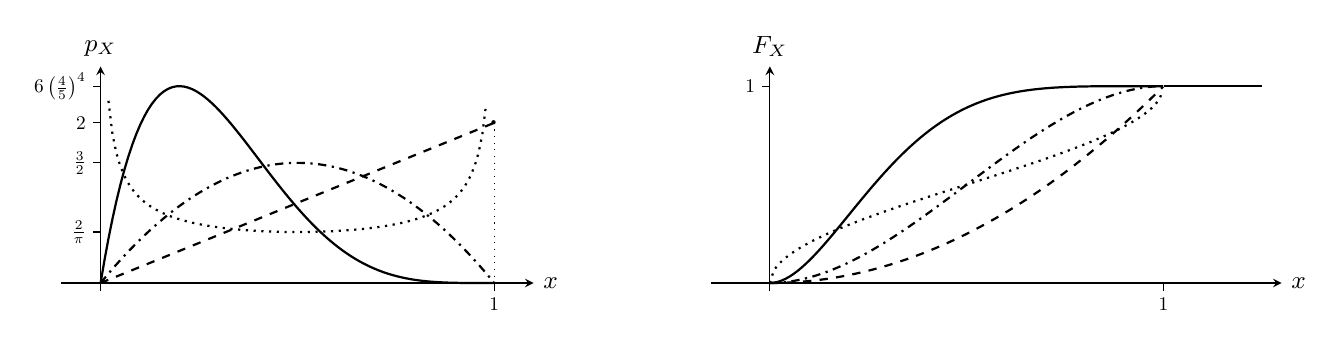
\begin{tikzpicture}%[scale=.9]
\shorthandoff{>}
%
\pgfmathsetmacro{\sx}{5};% x-scaling
\pgfmathsetmacro{\b}{5};% tercera eleccion de (2,beta)
\pgfmathsetmacro{\r}{.05};% radius arc non continuity F_X
%
%
% densidad
\begin{scope}
%
\pgfmathsetmacro{\sy}{2.5*((\b/(\b-1))^(\b-1))/(\b+1)};% y-scaling 
\draw[>=stealth,->] (-.5,0)--({\sx+.5},0) node[right]{\small $x$};
\draw[>=stealth,->] (0,-.1)--(0,2.75) node[above]{\small $p_X$};
%
%\draw[thick] (-.25,0)--(0,0);\draw (\r,\r) arc (90:270:\r);
%\draw[thick] (\sx,0)--({\sx+.25},0);\draw ({\sx-\r},{-\r}) arc (-90:90:\r);
% (a,b) = ( .5 , .5 )
\draw[thick,dotted,domain=.02:.98,samples=100] plot ({\x*\sx},{\sy*1/(pi*sqrt(\x*(1-\x)))});
% (a,b) = ( 2 , 1 )
\draw[thick,dashed,domain=0:1,samples=100] plot ({\x*\sx},{\sy*2*\x}) node[scale=.4]{$\bullet$};
\draw[dotted] (\sx,{2*\sy})--(\sx,0);
% (a,b) = ( 2 , 2 )
\draw[thick,dash dot,domain=0:1,samples=100] plot ({\x*\sx},{\sy*6*\x*(1-\x)});
% (a,b) = ( 2 , b_3 )
\draw[thick,domain=0:1,samples=100] plot ({\x*\sx},{\sy*\b*(\b+1)*\x*((1-\x)^(\b-1))});
%}
%
\draw (0,{\sy*2/pi})--(-.1,{\sy*2/pi}) node[left,scale=.7]{$\frac2\pi$};
\draw (0,{\sy*2})--(-.1,{\sy*2}) node[left,scale=.7]{$2$};
\draw (0,{\sy*1.5})--(-.1,{\sy*1.5}) node[left,scale=.7]{$\frac32$};
\draw (0,{\sy*(\b+1)*((1-1/\b)^(\b-1))})--(-.1,{\sy*(\b+1)*((1-1/\b)^(\b-1))}) node[left,scale=.7]{$6 \left(\frac{4}{5} \right)^4$};
\draw (\sx,0)--(\sx,-.1) node[below,scale=.7]{$1$};
%
\end{scope}
%
%
% reparticion
\begin{scope}[xshift=8.5cm]
%
\pgfmathsetmacro{\sy}{2.5};% y-scaling 
%
\draw[>=stealth,->] (-.75,0)--({\sx*1.25+.25},0) node[right]{\small $x$};
\draw[>=stealth,->] (0,-.1)--(0,{\sy+.25}) node[above]{\small $F_X$};
%
% cumulativa
\draw[thick] (-.5,0)--(0,0); \draw[thick] (\sx,\sy)--({\sx*1.25},\sy);
% (a,b) = ( .5 , .5 )
\draw[thick,dotted,domain=0:1,samples=100] plot ({\x*\sx},{\sy*(.5+asin(2*\x-1)/180)});
% (a,b) = ( 2 , 1 )
\draw[thick,dashed,domain=0:1,samples=100] plot ({\x*\sx},{\sy*(1-(1+\x)*(1-\x))});
% (a,b) = ( 2 , 2 )
\draw[thick,dash dot,domain=0:1,samples=100] plot ({\x*\sx},{\sy*(1-(1+2*\x)*((1-\x)^2))});
% (a,b) = ( 2 , b_3 )
\draw[thick,domain=0:1,samples=100] plot ({\x*\sx},{\sy*(1-(1+\b*\x)*((1-\x)^\b))});
%
\draw (0,\sy)--(-.1,\sy) node[left,scale=.7]{$1$};
\draw (\sx,0)--(\sx,-.1) node[below,scale=.7]{$1$};
\end{scope}
%
\end{tikzpicture} \end{center}
%
\leyenda{Ilustraci\'on de una densidad de  probabilidad beta (a), y la funci\'on
de  repartici\'on asociada (b).   $(a,b) =  (0.5 \,  , \,  0.5)$ (linea
punteada), $(3 \, , \, 1)$ (linea  mixta doble punteada), $(3 \, , \, 2)$ (linea
mixta), $(3 \, , \, 3)$ (linea
guionada), $(3 \, , \, 7)$ (linea llena).}
\label{Fig:MP:Beta}
\end{figure}

Notar que  se recupera la  ley uniforme sobre  \ $[0 \;  1]$ \ para  \ $a =  b =
1$. Se  conoce la ley de $  Y = 2 \,  B - 1$ \  con \ $B \,  \sim \, \beta\left(
  \frac12 , \frac12 \right)$ \ como {\em ley arcseno}.

Variables beta  tienen tambi\'en unas propiedades notables.  Primero, por cambio
de variables, se demuestra el lema siguiente:
%
\begin{lema}[Reflexividad]
\label{Lem:MP:ReflexividadBeta}
%
  Sea \ $X \, \sim \, \beta(a,b)$. Entonces
  %
  \[
  1-X \, \sim \, \beta(b,a)
  \]
  %
\end{lema}


\begin{lema}[Un v\'inculo con la ley exponencial]
\label{Lem:MP:VinculoBetaExponencial}
%
  Sea  \   $X  \,  \sim  \,   \beta(a,1)$. Entonces
  %
  \[
  - \log X \, \sim \, \E(a)
  \]
  %
\end{lema}
%
\begin{proof}
  El   resultado  es   inmediato  de   la  f\'ormula   de   transformaci\'on  del
  corolario~\ref{Cor:MP:TransformacionInyectivaDensidadEscalar}.
\end{proof}


\begin{lema}[Un v\'inculo con la ley uniforme]
\label{Lem:MP:VinculoBetaUniforme}
%
  Sea  \   $X  \,  \sim  \,   \U([0 \; 1])$ \ y \ $a > 0$. Entonces
  %
  \[
  U^{\frac{1}{a}} \, \sim \, \beta(a,1)
  \]
  %
\end{lema}
%
\begin{proof}
  El   resultado  es   inmediato  de   la  f\'ormula   de   transformaci\'on  del
  corolario~\ref{Cor:MP:TransformacionInyectivaDensidadEscalar}.
\end{proof}

\begin{lema}[Un v\'inculo con la ley gamma]
\label{Lem:MP:VinculoBetaGamma}
%
  Sea  \   $X  \,  \sim  \,   \G(a,c)$  \  e  \   $Y  \,  \sim   \,  \G(b,c)$  \
  independientes. Entonces
  %
  \[
  \frac{X}{X+Y} \, \sim \, \beta(a,b)
  \]
  %
  (independientemente  de $c$).   Adem\'as, $\frac{X}{X+Y}$  \ y  \ $X+Y$  \ son
  independientes.
\end{lema}
%
\begin{proof}
  La independencia de \ $c$ \ es obvia del hecho de que para cualquier $\theta >
  0, \: \theta^{-1} X \, \sim \, \G(a,\theta c)$ \ e \ $\theta^{-1} Y \, \sim \,
  \G(b,\theta  c)$,  la independencia  con  respecto  a \  $c$  \  viniendo de  \
  $\frac{\theta^{-1}     X}{\theta^{-1}     X     +     \theta^{-1}     Y}     =
  \frac{X}{X+Y}$.  Entonces, se  puede considerar  \ $c  = 1$  \ sin  perdida de
  generalidad. Ahora, sea la transformaci\'on
  %
  \[
  \begin{array}{lccl}
    g\ : & \Rset_+^2 & \mapsto & [0 \; 1] \times \Rset_+\\[1.5mm]
    %
    & (x,y) & \to & (u,v) = \left( \frac{x}{x+y} \, , \, x+y \right)
  \end{array}
  \]
  %
  Entonces, la transformaci\'on inversa se escribe
  %
  \[
  g^{-1}(u,v) = \left( u v \, , \, (1-u) v \right)
  \]
  %
  de matriz Jacobiana
  %
  \[
  \Jac_{g^{-1}} = \begin{bmatrix} v & u \\[2mm] -v & 1-u \end{bmatrix}
  \]
  %
  Del          teorema          de          cambio         de          variables
  teorema~\ref{Teo:MP:TransformacionBiyectiva},      notando     que     $\left|
    \Jac_{g^{-1}} \right| =  v$ \ y de la  independencia de \ $X$ \ e  \ $Y$, se
  obtiene para el vector aleatorio \ $W = \begin{bmatrix} U & V \end{bmatrix}^t$
  \ la densidad de probabilidad, definida sobre $[0 \; 1] \times \Rset_+$, como
  %
  \begin{eqnarray*}
    p_W(u,v) & = & p_X( u v ) \, p_Y( (1-u) v ) \, v\\[2mm]
    %
    & = & \frac{\left( u v \right)^{a-1} \, e^{- u v}}{\Gamma(a)} \times
    \frac{\left( (1-u) v \right)^{b-1} \, e^{- (1-u) v}}{\Gamma(b)} \times v\\[2mm]
    %
    & = & \frac{u^{a-1} (1-u)^{b-1}}{B(a,b)} \times \frac{v^{a+b-1} e^{-v}}{\Gamma(a+b)}
  \end{eqnarray*}
  %
  Inmediatamente, factorizandose, aparece  claramente que \ $U$ \ y  \ $V$ \ son
  independientes. Adem\'as, se reconoce en  el primer factor la densidad beta de
  par\'ametros $(a,b)$.   Pasando, se recupera  el hecho que  \ $X+Y \,  \sim \,
  \G(a+b,1)$.
\end{proof}

\begin{lema}[Stabilidad por producto]
\label{Lem:StabilidadBeta}
%
  Sea  \  $X \,  \sim  \, \beta(a,b)$  \  e  \ $Y  \,  \sim  \, \beta(a+b,c)$  \
  independientes. Entonces
  %
  \[
  X Y \, \sim \, \beta(a,b+c)
  \]
  %
\end{lema}
%
\begin{proof}
  Sean \ $U  \, \sim \, \G(a,1)$, \ $V \,  \sim \, \G(b,1)$ \ y \  $W \, \sim \,
  \G(c,1)$   \   independientes  y   sean   \   $X   =  \frac{U}{U+V}$,   $Y   =
  \frac{U+V}{U+V+W}$  \ y  \ $Z  = U+V+W$.  Del lema  anterior \  $X \,  \sim \,
  \beta(a,b)$ \ y \ $Y \, \sim \, \beta(a+b,c)$. Sea la transformaci\'on
  %
  \[
  \begin{array}{lccl}
    g\ : & \Rset_+^3 & \mapsto & [0 \; 1]^2 \times \Rset_+\\[1.5mm]
    %
    & (u,v,w) & \to & (x,y,z) = \left( \frac{u}{u+v} \, , \, \frac{u+v}{u+v+w} \, , \, u+v+w \right)
  \end{array}
  \]
  %
  Entonces, la transformaci\'on inversa se escribe
  %
  \[
  g^{-1}(x,y,z) = \left( x y z \, , \, (1-x) y z \, , \, z (1-y) \right)
  \]
  %
  de matriz Jacobiana
  %
  \[
  \Jac_{g^{-1}} = \begin{bmatrix}
  %
    y z  &   x z   &   x y   \\[2mm]
  %
  - y z  & (1-x) z & (1-x) y \\[2mm]
  %
    0    &  - z    &  1-y
  %
  \end{bmatrix}
  \]
  %
  De      nuevo,      del      teorema      de     cambio      de      variables
  teorema~\ref{Teo:MP:TransformacionBiyectiva}, notando que $\left| \Jac_{g^{-1}}
  \right| = y  z^2$ \ y de la independencia  de \ $U, V, W$,  se obtiene para el
  vector aleatorio  \ $  T =  \begin{bmatrix} X &  Y &  Z \end{bmatrix}^t$  \ la
  densidad de probabilidad probabilidad
  %
  \begin{eqnarray*}
    p_T(x,y,z) & = & p_u( x y z ) \, p_V( (1-x) y z ) \, p_W( y (1-z) ) \, y z^2\\[2mm]
    %
    & = & \frac{\left( x y z \right)^{a-1} \, e^{- x y z}}{\Gamma(a)} \times
    \frac{\left( (1-x) y z \right)^{b-1} \, e^{- (1-x) y z}}{\Gamma(b)} \times
    \frac{\left( z (1-y) \right)^{c-1} \, e^{- z (1-y)}}{\Gamma(c)} \times y
    z^2\\[2mm]
    %
    & = & \frac{x^{a-1} (1-x)^{b-1}}{B(a,b)} \times \frac{y^{a+b-1}
      (1-y)^{c-1}}{B(a+b,c)} \times \frac{z^{a+b+c-1} e^{-z}}{\Gamma(a+b+c)}
  \end{eqnarray*}
  %
  Eso proba  que \  $X, \ Y$  \ y  $Z$ \ son  independientes (las  densidades se
  factorizan). Adem\'as,
  %
  \[
  X  Y =  \frac{U}{U+V} \times  \frac{U+V}{U+V+W} =  \frac{U}{U+V+W} \,  \sim \,
  \beta(a,b+c)
  \]
  %
  el      \'ultimo       resultado      como      consecuencia       de      los
  lemas~\ref{Lem:MP:VinculoBetaGamma}    y~\ref{Lem:MP:StabilidadGamma}.     Eso
  cierra la prueba.
\end{proof}


\begin{lema}[Ley gamma como caso l\'imite de beta]
\label{Lem:GamaLimiteBeta}
%
  Sea \ $X_n \, \sim \, \beta(a,n)$. Entonces
  %
  \[
  n X_n \limitd{n \to +\infty} X \, \sim \, \G(a,1)
  \]
  %
  con \ $\displaystyle \limitd{}$ \ l\'imite es en distribuci\'on
\end{lema}
%
\begin{proof}
  De la f\'ormula de transformaci\'on tenemos la distribuci\'on de $n X_n$
  %
  \begin{eqnarray*}
  p_{n X_n}(x) & = & \frac{1}{n} , \frac{\left( \frac{x}{n} \right)^{a-1} \left( 1
  - \frac{x}{n} \right)^{n-1}}{B(a,n)} \, \un_{(0 \; 1)}\left( \frac{x}{n} \right)\\[2mm]
  %
  & = & \frac{x^{a-1}}{\Gamma(a)} \: \frac{\Gamma(n+a)}{n^a \Gamma(n)} \: \left( 1 -
  \frac{x}{n} \right)^{n-1} \: \un_{(0 \; n)(x)}
  \end{eqnarray*}
  %
  El resultado sigue  notando que \ $\un_{(0 \;  n)} \to \un_{\Rset_{0,+}}$, \quad
  $\left(  1 -  \frac{x}{n} \right)^{n-1}  \to e^{-x}$  \ y  de la  f\'ormula de
  Stirling (ver secci\'on~\ref{Sssec:MP:Poisson}).
\end{proof}

\

La distribuci\'on beta  se generaliza al caso matriz-variada  $X$ definido sobre
$\X$ tal que $X$ y $I-X$ partenecen  a $\Pos_d^+(\Rset)$; se denota \ $X \, \sim
\, \beta_d(a,b)$ \ donde  \ $(a,b) \in \Rset_+^{* \, 2}$ y  la densidad est dada
por   $\displaystyle  p_X(x)   =  \frac{|x|^{a   -  \frac{d+1}{2}}   |I-x|^{b  -
    \frac{d+1}{2}}}{B_p\left([a  \quad  b]^t\right)},  \quad  (a,b)  \in  \left(
  \frac{d-1}{2} \; +\infty \right)^2$. Se refiera a~\cite[Cap.~5]{GupNag99} para
tener m\'as detalles.   Notar que esta distribuci\'on cae en  en una clase dicha
el\'iptica,      que      vamos       a      ver      brevemente      en      la
secci\'on~\ref{Ssec:MP:FamiliaElipticaMatriz},  as\'i  que  propiedades en  este
marco general.



% --------------------------------- Dirichlet
\subsubseccion{Distribuci\'on de Dirichlet}
\label{Sssec:MP:Dirichlet}

Esta distribuci\'on teniendo su nombre de integrales on a simplex estudiados por
M. Lejeune-Dirichlet y J. Liouville  en 1839~\cite{GupRic01, Dir39, Lio39} en es
una extensi\'on  multivariada de las variables  beta a veces  conocida como {\em
  Beta multivariada}~\cite{OlkRub64}. Se  nota \ $X \, \sim \,  \Dir(a)$ \ con \
$a \in \Rset_+^{*  \, k}$ \ y \  $X$ \ vive sobre el  $(k-1)$-simplex estandar \
$\Simp{k-1}$.  $a$ es  llamado parametro de forma. Como en  el caso de vectores
de  distribuci\'on multinomial, a  pesar de  que se  escribe \  $X$ \  de manera
$k$-dimensional, el vector partenece a una  variedad \ $d = k-1$ \ dimensional y
en el caso  \ $k = 2$ \ se  recupera la ley beta. A veces  se parametriza la ley
con un  parametro escalar \ $\alpha  > 0$ \ y  un vector del  simplex estandar \
$\bar{a} \in \Simp{k-1}$ \ tal que
%
\[
a = \alpha \bar{a}, \quad \mbox{\ie} \quad \alpha = \sum_{i=1}^k \alpha_i, \quad
\bar{a} = \frac{a}{\alpha}
\]
%
$\alpha$ \  es conocido como  parametro de {\em  concentraci\'on} y el  vector \
$\bar{a}$ \ como {\em medida de base}.

Las caracter\'isticas de un vector de Dirichlet son:

\begin{caracteristicas}
%
Dominio de definici\'on~\footnote{De hecho, se puede considerar que el vector
aleatorio es \ $(k-1)$-dimensional \ $\widetilde{X} = \begin{bmatrix}
\widetilde{X}_1 & \cdots & \widetilde{X}_{k-1} \end{bmatrix}^t$ \ definido sobre
el hipertriangulo \ $\widetilde{\X} = \Tri_{k-1} = \left\{ \widetilde{x} \in [0
\; 1]^{k-1}, \: \sum_{i=1}^{k-1} \widetilde{x}_i \le 1 \right\}$, proyecci\'on
del simplex sobre el hiperplano \ $x_k = 0$.\label{Foot:MP:DirichletXtilde}} &
$\X = \Simp{k-1}, \: k \in \Nset \setminus \{ 0 \; 1 \}$\\[2mm]
\hline
%
Parametros & $a = \alpha \, \bar{a} \, \in \, \Rset_+^{* \, k}$ \ (forma) \ con
\ $\alpha \in \Rset_+^*$ \ (concentraci\'on) y \ $\bar{a} \in \Simp{k-1}$
(medida de base)\\[2mm]
\hline
%
Densidad de probabilidad~\footnote{La densidad de probabilidad es dada con
respeto a la medida de Lebesgue restricta al simplex \ $\Simp{k-1}$. Tratando
de \ $\widetilde{X}$, el vector tiene una densidad con respeto a la medida de
Lebesgue usual, y es dada por \ $p_{\widetilde{X}}\left( \widetilde{x} \right) =
\frac{\prod_{i=1}^{k-1} \widetilde{x}_i^{\, a_i-1} \, \left( 1 -
\sum_{i=1}^{k-1} \widetilde{x}_i
\right)^{a_k-1}}{B(a)}$.\label{Foot:MP:DirichletDensidad}} & $\displaystyle
p_X(x) = \frac{\prod_{i=1}^k x_i^{a_i-1}}{B(a)}$\\[2mm]
\hline
%
Promedio & $\displaystyle m_X = \bar{a}$\\[2.5mm]
%\frac{a}{\sum_{i=1}^k a_i} \equiv \overline{a}$\\[2.5mm]
\hline
%
Covarianza & $\displaystyle \Sigma_X = \frac{\diag\left( \bar{a} \right) -
\bar{a} \bar{a}^t}{1 + \alpha}$\\[2.5mm]
%\sum_{i=1}^k a_k}$\\[2.5mm]
\hline
%
Generadora de momentos~\footnote{El v\'inculo entre las funciones generadoras de
momento de \ $X$ \ y \ $\widetilde{X}$ \ es trivialmente \
$M_{\widetilde{X}}\left( \widetilde{u} \right) = M_X\left( \begin{bmatrix}
\widetilde{u} & 0 \end{bmatrix}^t \right)$ \ o \ $M_X(u) = e^{\imath u_k}
M_{\widetilde{X}}\left( \begin{bmatrix} u_1 - u_k & \cdots & u_{k-1} -
u_k \end{bmatrix}^t \right)$, y similarmente para la funci\'on
caracter\'istica.\label{Foot:MP:Dirichlet}} & $\displaystyle M_X(u) =
\Phi_2^{(k)}( a , \alpha \, ; \, u )$ \ para \ $u \in \Cset$\\[2mm]
\hline
%
Funci\'on caracter\'istica~\footnote{La forma de la funci\'on generadora de
momento viene directamente de la escritura de las series de Taylor de $e^{u_i
x_i}$ \ o de la forma integral de la funci\'on confluente
hipergeom\'etrica~\cite{Phi88}.} & $\displaystyle \Phi_X(\omega) = \Phi_2^{(k)}(
a , \alpha \, ; \, \imath \omega )$
\end{caracteristicas}

%$k$-variada~\footnote{$\Phi_2^{(k)}(a;b;z)     =     \sum_{m    \in     \Nset^k}
%  \frac{(a_1)_{(m_1)}     \ldots    (a_k)_{(m_k)}     \,     z_1^{m_1}    \ldots
%    z_k^{m_k}}{(b)_{(m_1+\cdots+m_k)} m_1!  \ldots m_k!}$  \ con \ $(x)_{(n)}$ \
%  s\'imbolo  de Pochhammer  usual o  factorial creciente,  $(x)_{(n)} =  x (x+1)
%  \ldots (x+n)$ \,  con la convenci\'ion \ $(x)_{(0)} = 1$.   De hecho, la forma

La figura Fig.~\ref{Fig:MP:Dirichlet} representa  el dominio de definici\'on del
vector (a) y su densidad de  probabildad con las marginales (ver m\'as adelante)
para $k = 3$.
%
\begin{figure}[h!]
\begin{center} \begin{tikzpicture}%[scale=.8]
\shorthandoff{>}
%
\tikzset{declare function={
xplus(\x) = max(\x,0);
%ifthenelse(\x > 0 , \x , NaN);
}}
%}

% Simplex
\tdplotsetmaincoords{45}{65}
\begin{scope}[tdplot_main_coords,scale=.75]
%
% Dirichlet: \X = S_{k-1} y \widetilde{X}
\pgfmathsetmacro{\dx}{3};% scaling
%
\draw[->,>=stealth] (-.25,0,0)--({\dx+.5},0,0) node[below right,scale=.9]{$x_1$};
%\node at (\dx,0,0)[left,scale=.8]{$1$};
\draw (\dx,0,0)--(\dx,-.15,0) node[left,scale=.8]{$1$};
%
\draw[->,>=stealth] (0,-.25,0)--(0,{\dx+.5},0) node[right,scale=.9]{$x_2$};
%\node at (0,\dx,0)[below,scale=.8]{$1$};
\draw (0,\dx,0)--(.15,\dx,0) node[below,scale=.8]{$1$};
%
\draw[->,>=stealth] (0,0,-.25)--(0,0,{\dx+.5}) node[above,scale=.9]{$x_3$};
%\node at (0,0,\dx)[left,scale=.8]{$1$};
\draw (0,0,\dx)--(0,-.15,\dx) node[left,scale=.8]{$1$};
%
\node at (0,0,0)[below left,scale=.8]{$0$};
%
% tilde X
\filldraw[fill=black!50,opacity=.5] (0,0,0)--(\dx,0,0)--(0,\dx,0);
\draw[thick,color=black,dashed] (0,0,0)--(\dx,0,0)--(0,\dx,0)--(0,0,0);
\node at ({\dx/15},{\dx/20},0)[right,scale=.7]{$\Tri_2$};
%
% Simplex Delta_2
\filldraw[fill=black!75,opacity=.5] (\dx,0,0)--(0,\dx,0)--(0,0,\dx);
\draw[thick,color=black] (\dx,0,0)--(0,\dx,0)--(0,0,\dx)--(\dx,0,0);
\node at ({.05*\dx},{.05*\dx},{.8*\dx})[right,scale=.7]{$\Simp{2}$};
%
\end{scope}
%
%
% densidad (3,2,2)
\begin{scope}[xshift=4cm,yshift=-2cm,scale=.75]
%
\pgfmathsetmacro{\au}{3};% a1
\pgfmathsetmacro{\ad}{2};% a2
\pgfmathsetmacro{\at}{2};% a3
\pgfmathsetmacro{\B}{factorial(\au-1)*factorial(\ad-1)*factorial(\at-1)/factorial(\au+\ad+\at-1)};% normalizacion
\pgfmathsetmacro{\Bu}{factorial(\au-1)*factorial(\ad+\at-1)/factorial(\au+\ad+\at-1)};% normalizacion 1
\pgfmathsetmacro{\Bd}{factorial(\ad-1)*factorial(\au+\at-1)/factorial(\au+\ad+\at-1)};% normalizacion 2
\pgfmathsetmacro{\ma}{((\au-1)^(\au-1))*((\ad-1)^(\ad-1))*((\at-1)^(\at-1))/((\au+\ad+\at-3)^(\au+\ad+\at-3))/\B};
%
% Dirichlet & marginales
\begin{axis}[
    colormap = {whiteblack}{color(0cm)  = (white);color(1cm) = (black)},
    width=.5\textwidth,
    view={45}{65},
    enlargelimits=false,
    %grid=major,
    domain=0:1,
    y domain=0:1,
    %unbounded coords=jump, % para tener un dominio no cuadrado
    %filter point/.code={%
    %\pgfmathparse
    %{\pgfkeysvalueof{/data point/x} + \pgfkeysvalueof{/data point/y} > 1.0}%
    %  \ifpgfmathfloatcomparison
    %     \pgfkeyssetvalue{/data point/x}{nan}%
    %  \fi
    %},
    zmax={.8*\ma},
    color=black,
    samples=70,
    xlabel=$x_1$,
    ylabel=$x_2$,
    zlabel=$p_{\widetilde{X}}$,
]
%
% Dirichlet
\addplot3 [surf] {(x^(\au-1))*(y^(\ad-1))*(xplus(1-x-y)^(\at-1))/\B};
%
% Marginales
\addplot3 [domain=0:1,samples=50, samples y=0, thick, smooth, color=black] (x,1,{(x^(\au-1))*((1-x)^(\ad+\at-1))/\Bu});
\addplot3 [domain=0:1,samples=50, samples y=0, thick, smooth, color=black] (0,x,{(x^(\ad-1))*((1-x)^(\au+\at-1))/\Bd});
%
\node at (axis cs:.5,1,{1/(2^(\au+\ad+\at-2))/\Bu})[right]{$p_{X_1}$};
\node at (axis cs:0,.5,{1/(2^(\au+\ad+\at-2))/\Bd})[above]{$p_{X_2}$};
\end{axis}
\end{scope}
%
%
% densidad (3,2,2)
\begin{scope}[xshift=11cm,yshift=-2cm,scale=.75]
%
\pgfmathsetmacro{\au}{3};% a1
\pgfmathsetmacro{\ad}{1};% a2
\pgfmathsetmacro{\at}{2};% a3
\pgfmathsetmacro{\B}{factorial(\au-1)*factorial(\ad-1)*factorial(\at-1)/factorial(\au+\ad+\at-1)};% normalizacion
\pgfmathsetmacro{\Bu}{factorial(\au-1)*factorial(\ad+\at-1)/factorial(\au+\ad+\at-1)};% normalizacion 1
\pgfmathsetmacro{\Bd}{factorial(\ad-1)*factorial(\au+\at-1)/factorial(\au+\ad+\at-1)};% normalizacion 2
\pgfmathsetmacro{\ma}{((\au-1)^(\au-1))*((\ad-1)^(\ad-1))*((\at-1)^(\at-1))/((\au+\ad+\at-3)^(\au+\ad+\at-3))/\B};
%
\begin{axis}[
    colormap = {whiteblack}{color(0cm)  = (white);color(1cm) = (black)},
    width=.5\textwidth,
    view={45}{65},
    enlargelimits=false,
    %grid=major,
    domain=0:1,
    y domain=0:1,
    zmax={.65*\ma},
    color=black,
    samples=70,
    xlabel=$x_1$,
    ylabel=$x_2$,
    zlabel=$p_{\widetilde{X}}$,
]
%
% Dirichlet
\addplot3 [surf,opacity=.8] {(x^(\au-1))*(y^(\ad-1))*(xplus(1-x-y)^(\at-1))/\B};
%
% Marginales
\addplot3 [domain=0:1,samples=50, samples y=0, thick, smooth, color=black] (x,1,{(x^(\au-1))*((1-x)^(\ad+\at-1))/\Bu});
\addplot3 [domain=0:1,samples=50, samples y=0, thick, smooth, color=black] (0,x,{(x^(\ad-1))*((1-x)^(\au+\at-1))/\Bd});%
%
\node at (axis cs:.5,1,{1/(2^(\au+\ad+\at-2))/\Bu})[right]{$p_{X_1}$};
\node at (axis cs:0,.5,{1/(2^(\au+\ad+\at-2))/\Bd})[above]{$p_{X_2}$};
\end{axis}
\end{scope}
%
\node at (1.2,-3){(a)};
\node at (6.6,-3){(b)};
\node at (13.6,-3){(c)};
\end{tikzpicture} \end{center}
%
\leyenda{Ilustraci\'on del  dominio $\Simp{k-1}$ de  definici\'on de la  ley de
  Dirichlet   para  \   $k  =   3$   \  (grise   oscuro),  con   el  dominio   \
  $(k-1)$-dimensional   \  $\Tri_{k-1}$   \  del   vector  \   $\widetilde{X}  =
  \protect\begin{bmatrix}   X_1  &  X_2   \protect\end{bmatrix}^t$  \   ($X_3  =
  1-X_1-X_2$) \ (grise claro) (a), y densidad de probabilidad de $\widetilde{X}$
  \   con   las   marginales   \   $p_{X_1},   \:   p_{X_2}$   (ver   notas   de
  pie~\ref{Foot:MP:DirichletDominio}   y~\ref{Foot:MP:DirichletDensidad}).   Los
  parametros   son    \   $a   =    \protect\begin{bmatrix}   3   &   2    &   2
    \protect\end{bmatrix}^t$  (b) y \  $a =  \protect\begin{bmatrix} 3  & 1  & 2
    \protect\end{bmatrix}^t$ (c).}
\label{Fig:MP:Dirichlet}
\end{figure}


Vectores  de  distribuci\'on  de  Dirichlet tienen  tambi\'en  unas  propiedades
notables, parecidas a las de la beta:
%
\begin{lema}[Reflexividad]\label{Lem:MP:ReflexividadDir}
%
  Sea  \ $X \,  \sim \,  \Dir(a), \:  a \in  \Rset_+^{* \,  k}$ \  y \  $\Pi \in
  \mathfrak{S}_k(\Rset)$ \ matriz \ de permutaci\'on. Entonces
  %
  \[
  \Pi X \, \sim \, \Dir\left( \Pi a \right)
  \]
  %
\end{lema}

%
\begin{proof}
  El resultado es inmediato por cambio  de variables $x \to \Pi x$, la Jacobiana
  siende   $\Pi$,   de   valor   absoluto   determinente  igual   a   $1$   (ver
  secci\'on~\ref{Sec:MP:Transformacion}).
\end{proof}
%
Adem\'as, se muestra una stabilidad remplazando dos componentes por su suma:
%
\begin{lema}[Stabilidad por agregaci\'on]\label{Lem:MP:StabSumaDir}
%
  Sea  \ $X =  \begin{bmatrix} X_1  & \cdots  & X_k  \end{bmatrix}^t \,  \sim \,
  \Dir(a),  \:  a =  \begin{bmatrix}  a_1 &  \cdots  &  a_k \end{bmatrix}^t  \in
  \Rset_+^{*  \,  k}$  \  y  \  $G^{(i,j)}$ \  matriz  de  agrupaci\'on  de  las
  $(i,j)$-\'esima componentes (ver notaciones). Entonces,
  %
  \[
  G^{(i,j)} X \, \sim \, \Dir\left( G^{(i,j)} a \right)  
  \]
  %
\end{lema}
%
\begin{proof}
  Se  puede probar  este resultado  a partir  de la  funci\'on caracter\'istica,
  usando      las      propiedades      de      la      funci\'on      confluent
  hipergeom\'etrica~\cite{SriKar85, Hum22, App25,  AppKam26, Erd37, Erd40}. Pero
  se  puede tambi\'en  tener un  enfoque m\'as  directo.  Del  lema precediente,
  notando que existe una matriz de  permutaci\'on \ $\Pi$ \ tal que \ $G^{(i,j)}
  = G^{(1,2)} \Pi$, se  puede concentrarse en el caso \ $(i,j)  = (1,2)$. Sea el
  cambio de  variables $g: x =  (x_1,\ldots,x_k) \mapsto u  = (u_1,\ldots,u_k) =
  (x_1,x_1+x_2,x_3,\ldots,x_k)$.        Entonces       \      $g^{-1}(u)       =
  (u_1,u_2-u_1,u_3,\ldots,u_k)$ \ es de determinente de matriz Jacobiana igual a
  \ $1$ \ dando para $U = g(X)$ \ la densidad
  %
  \[
  p_U(u)  = \frac{u_1^{a_1-1}  \left(  u_2 -  u_1 \right)^{a_2-1}  \prod_{i=3}^k
    u_i^{a_i-1}}{B(a)}
  \]
  %
  sobre $g\left(  \Simp{k-1} \right)$. Para $u_2  \in [0 \; 1]$  \ tenemos $u_1
  \in [  0 \;  u_2]$ \ as\'i  que, por  marginalizaci\'on en $u_1$  obtenemos la
  densidad
  %
  \begin{eqnarray*}
  p_{G^{(1,2)} X}(u_2,\ldots,u_k) & = & \frac{\prod_{i=3}^k u_i^{a_i-1}}{B(a)}
  \int_0^{u_2} u_1^{a_1-1} \left( u_2 - u_1 \right)^{a_2-1} \, du_1\\[2mm]
  %
  & = & \frac{\prod_{i=3}^k u_i^{a_i-1}}{B(a)} \, u_2^{a_1+a_2-1} \int_0^1
  v_1^{a_1-1} \left( 1 - v_1 \right)^{a_2-1} \, dv_1
  \end{eqnarray*}
  %
  con el cambio de variables $u_1 = u_2 v_1$. Se cierra la prueba notando que la
  integral   vale  \  $B(a_1,a_2)$   \  y   que  \   $\frac{B(a_1,a_2)}{B(a)}  =
  \frac{1}{B\left( G^{(1,2)} a \right)}$.
\end{proof}

De este lema, aplicado de manera recursiva, se obtiene en corolario siguiente:
%
\begin{corolario}
\label{Cor:MP:MarginalDirichletBeta}
%
  Sea  \ $X  \,  \sim \,  \Dir(a)$, entonces  \  $\displaystyle X_i  \, \sim  \,
  \beta\left( a_i \, , \, \alpha-a_i \right)$.
\end{corolario}

Naturalmente,  la ley de  Dirichelt siendo  una extensi\'on  de la  beta, existe
tambi\'en un v\'inculo entre esta ley y variables de distribuci\'on gamma:
%
\begin{lema}[V\'inculo con la ley gamma]
\label{Lem:MP:VinculoDirichletGamma}
%
Sea \ $X$ \ vector $k$-dimensional de componente \ $i$-\'esima \ $X_i \, \sim \,
\G(a_i,c), \: i = 1, \ldots , k$ \ independientes \ y \ $a$ vector de componente
$i$-\'esima \ $a_i$. Entonces
  %
  \[
  \frac{X}{\sum_{i=1}^k X_i} \, \sim \, \Dir(a)
  \]
  %
  (independientemente  de $c$).   Adem\'as, $\frac{X}{\sum_{i=1}^k  X_i}$ \  y \
  $\sum_{i=1}^k X_i$ \ son independientes.
\end{lema}
%
\begin{proof}
  La    prueba   sigue    exactamente   los    mismos   pasos    que    la   del
  lema~\ref{Lem:MP:VinculoBetaGamma} \ trabajando con \ $\widetilde{X}$.
\end{proof}

Naturalmente,  la  distribuci\'on de  Dirichlet,  extensi\'on  de  la ley  beta,
aparece entre  otros en problema  de inferencia Bayesiana como  distribuci\'on a
priori  conjugado~\footref{Foot:MP:BayesPrior}  del  parametro  $p$  de  la  ley
multinomial~\cite{Rob07}, extensi\'on de la ley binomial.

\SZ{
Polya urn schemes, Chinese restaurant
}


La distribuci\'on de Dirichlet se generaliza al caso matriz-variada $X$ definido
sobre $\P_{d,k}(\Rset)$,  conjuntos de  $k$-uplet de matrices  de $P_d^+(\Rset)$
cumpliando la relaci\'on  de completud (ver notaciones); se denota  \ $X \, \sim
\, \Dir_d(a)$  \ donde \  $a \in \left(  \frac{d-1}{2} \; +\infty  \right)^k$ la
densidad  est dada por  $\displaystyle p_X(x)  = \frac{\prod_{i=1}^k  \left| x_i
  \right|^{a_i-\frac{d+1}{2}}}{B_d(a)}$.   Se  refiera a~\cite[Cap.~6]{GupNag99}
para tener m\'as informaciones.


% --------------------------------- Student-t
\subsubseccion{Distribuci\'on Student-$t$ multivariada}
\label{Sssec:MP:StudentT}

En   el  caso   escalar,  esta   ley   fue  introducida   inicialmente  por   F.
R. Helmert~\cite{Hel75, Hel76, She95}  y J.  L\"uroth~\cite{Lur76, Pfa96}.  Pero
es m\'as  conocida por su  introducci\'on por William  Sealy Gosset~\footnote{De
  hecho, W.  S.  Gosset fue un estudiante trabajando en  la f\'abrica de cerveza
  irlandesa  Guiness sobre  estad\'isticas  relacionadas a  la  qu\'imica de  la
  cerveza.  Hay  varias versiones sobre el  hecho que se  public\'o este trabajo
  bajo  el nombre  ``Student''.  Una  es que  fue  para que  no se  sabe que  la
  f\'abrica  estaba  trabajando  sobre  estas estad\'isticas  para  estudiar  la
  calidad   de   la   cerveza~\cite{Wen16}.\label{Foot:MP:Student}}   en   1908,
trabajando  sobre variables centradas  normalizadas por  el promedio  y varianza
emp\'iricos~\cite{Stu08}.   Fue  estudiada  entre  otros intensivamente  por  el
famoso  matem\'atico R.   Fisher~\cite{Fis25}.  En  la literatura,  esta  ley es
conocida bajo  los nombres {\em  Student}, {\em Student-$t$} o  simplemente {\em
  $t$-distribuci\'on} o  a\'un bajo el nombre  {\em Pearson tipo IV}  en el caso
escalar  y {\em  Pearson tipo  VII}  (para $\frac{\nu+d}{2}$  entero; ver  m\'as
abajo), debido  a la  familia de Pearson~\cite{Pea95,  JohKot95:v1, JohKot95:v1,
  KotBal00, FanKot90}.   Esta distribuci\'on aparece como a  priori conjugado de
la media de una gaussiana en inferencia bayesiana~\cite{Rob07, KotNad04}.

Se denota con \ $X \sim \T_\nu(m,\Sigma)$ \ con \ $m \in \Rset^d$, \ $\Sigma \in
\Pos_d^+(\Rset)$ \ conjunto  de las matrices de \  $\Mat_{d,d}(\Rset)$ \ sim\'etricas
definidas positivas. $m$ \ es llamado  {\em par\'ametro de posici\'on} (no es la
media   que  puede  no   existir),  \   $\Sigma$  \   es  llamada   {\em  matriz
  caracter\'istica} (no es [proporcional a]  la covarianza que puede no existir)
y \ $\nu > 0$ \ llamado  {\em grado de libertad}.  Las caracter\'isticas de una
Student-$t$ son las siguientes:
%
\begin{caracteristicas}
%
Dominio de definici\'on & $\X = \Rset^d$\\[2mm]
\hline
%
Par\'ametro & $\nu \in \Rset_{0,+}$ \ (grado de libertad), \ $m \in \Rset^d$ \
(posici\'on), \ $\Sigma \in \Pos_d^+(\Rset)$ \ (matriz caracter\'istica)\\[2mm]
\hline
%
Densidad de probabilidad & $\displaystyle p_X(x) = \frac{\Gamma\left(
\frac{\nu+d}{2} \right)}{\pi^{\frac{d}{2}} \nu^{\frac{d}{2}} \Gamma\left(
\frac{\nu}{2} \right) \, \left| \Sigma \right|^{\frac12}} \, \left( 1 +
\frac{(x-m)^t \Sigma^{-1} (x-m)}{\nu} \right)^{- \, \frac{\nu+d}{2}}$\\[2mm]
\hline
%
Promedio & $\displaystyle m_X = m$ \ si \ $\nu > 1$; \ no
existe si no~\footnote{De manera general, esta ley admite momentos de orden \ $k$ \
si y solamente si \ $\nu > k$.\label{Foot:MP:ExistenciaMomentosStudent}}.\\[2.5mm]
\hline
%
Covarianza~\footnote{Fijense de que $\Sigma$ no es la covarianza, pero es
proporcional a la covarianza\ldots cuando existe. Se podr\'ia imaginar
renormalizar la ley tal que \ $\Sigma_X$ \ y \ $\Sigma$ \ coinciden, pero no
ser\'ia posible en el caso \ $\nu \le 2$.} & $\displaystyle \Sigma_X =
\frac{\nu}{\nu-2} \, \Sigma$ \ si \ $\nu > 2$; \ no existe si
no~\footref{Foot:MP:ExistenciaMomentosStudent}.\\[2.5mm]
\hline
%
\modif{Asimetr\'ia} & $\displaystyle \gamma_X = 0$ \ si \ $\nu > 3$; \ no existe
si no~\footref{Foot:MP:ExistenciaMomentosStudent}.\\[2mm]
\hline
%
Curtosis por exceso & \modif{$\displaystyle \widebar{\kappa}_X = \frac{2}{\nu-4}
\Big( I \otimes I + \tau_{(2,3)}\big[ I \otimes I \big] + \tau_{(2,4)}\big[ I
\otimes I \big] \Big)$
%\sum_{i,j=1}^d \Big( \! \left( % \un_i \un_i^t \right) \otimes \left( \un_j
%\un_j^t \right) + \left( \un_i % \un_j^t \right) \otimes \left( \un_i \un_j^t
%\right) + \left( \un_i \un_j^t % \right) \otimes \left( \un_j \un_i^t \right) \!
%\Big)$
}\newline si \ $\nu >
4$; \ no existe si no~\footref{Foot:MP:ExistenciaMomentosStudent}.\\[2mm]
\hline
%
Funci\'on caracter\'istica~\footnote{Se  muestra sencillamente que  la funci\'on
  generatriz de  momentos puede existir si y  solamente si \ $\real{u}  = 0$. La
  funci\'on generadora de momentos restricta  al producto cartesiano de rectas \
  $\real{u} =  0$ \ es nada  m\'as que la  funci\'on caracter\'istica. Adem\'as,
  esta  funci\'on  fue  calculdada,   especialmente  en  el  caso  multivariado,
  relativamente   recientemente~\cite{Sut86,  Hur95,  KibJoa06,   SonPar14}.}  &
$\displaystyle  \Phi_X(\omega)  = \frac{\nu^{\frac{\nu}{4}}}{2^{\frac{\nu}{2}-1}
  \Gamma\left(  \frac{\nu}{2}  \right)}  \,  e^{\imath  \omega^t  m}  \,  \left(
  \omega^t   \Sigma   \omega   \right)^{\frac{\nu}{4}}   K_{\frac{\nu}{2}}\left(
  \sqrt{\nu \, \omega^t \Sigma \omega} \right)$
\end{caracteristicas}

Nota: nuevamente se puede escribir $X \, \egald \, \Sigma^{\frac12} S + m$ \ con
\ $S \, \sim \, \T_\nu(0,I)$ \  donde \ $S$ \ es dicha {\em Student-$t$ estandar}
y  las caracter\'isticas  de \  $X$  \ son  v\'inculadas a  las  de \  $S$ \  (y
vice-versa) por transformaci\'on lineal (ver secciones anteriores).

Densidades  de probabilidad  Student-$t$ estandar  y funciones  de repartici\'on
asociadas   en    el   caso   escalar    son   representadas   en    la   figura
Fig.~\ref{Fig:MP:StudentT}-(a) y  (b) para  varios $\nu$, y  una densidad  en un
contexto bi-dimensional figura Fig.~\ref{Fig:MP:StudentT}(c).
%
\begin{figure}[h!]
\begin{center} \begin{tikzpicture}
\shorthandoff{>}
%
% Para el caso univariado
\pgfmathsetmacro{\sx}{.43};% x-scaling
\pgfmathsetmacro{\mu}{0};% para tomar los grados de libertad impar; 0 => Cauchy
\pgfmathsetmacro{\md}{1};
\pgfmathsetmacro{\mt}{3};
%\pgfmathsetmacro{\mq}{3};
%
%
% para el caso bi-variado
\pgfmathsetmacro{\mdd}{0};%
\pgfmathsetmacro{\nu}{2*\mdd+1};% grados de libertad
\pgfmathsetmacro{\a}{1/3};% x-scaling
\pgfmathsetmacro{\t}{30};% angulo de rotacion
\pgfmathsetmacro{\c}{cos(\t)};% coseno
\pgfmathsetmacro{\s}{sin(\t)};% seno
\pgfmathsetmacro{\su}{sqrt(\c^2+(\a*\s)^2)};% ecart-type 1
\pgfmathsetmacro{\sd}{sqrt(\s^2+(\a*\c)^2)};% ecart-type 2
\pgfmathsetmacro{\dx}{3};% dominio x del plot -dx:dx
\pgfmathsetmacro{\dy}{2.5};% dominio y del plot -dy:dy
%
%
% Approximacion de la funcion Gamma
%\tikzset{declare function={gamma(\z)=
%(2.506628274631*sqrt(1/\z) + 0.20888568*(1/\z)^(1.5) + 0.00870357*(1/\z)^(2.5) -
%(174.2106599*(1/\z)^(3.5))/25920 - (715.6423511*(1/\z)^(4.5))/1244160)*exp((-ln(1/\z)-1)*\z);}}
%
% Approximation de la cdf gaussienne
\tikzmath{function normcdf(\x) {return 1/(1 + exp(-0.07056*(\x)^3 - 1.5976*(\x)));};};
%
% coefficiente binomial, para no tener factoriales muy grandes
\tikzmath{function binocoef(\m,\k) {if \k == 0 then {return 1;} else {return ((\m-\k+1)/\k)*binocoef(\m,\k-1);};};};
%
% coefficient que aparece en la pdf y cdf (ver doubling formula GraRyz 8.335-5 con x = m+1/2)
% y coefficiente de normalizacion
%\tikzset{declare function={
\tikzmath{function coefstud(\m) {return (4^\m)/(pi*sqrt(2*\m+1)*binocoef(2*\m,\m));};}
%
%
% cdf Student que se calcula recursivamente para nu = 2 m + 1, m entero
\tikzmath{function studcdfS(\x,\k) {
    if \k == 0 then {return .5+(atan(\x))/180;}
    else {return studcdfS(\x,\k-1)+((4^\k)*(\x)/(2*pi*\k*binocoef(2*\k,\k)))/((1+((\x)^2))^\k);};
};};
% Calculo de
%  - x maximo del plot para tener pdf a 7% del max
%  - la pdf Student para nu = 2 m + 1, m entero
%  - la cdf Student para nu = 2 m + 1, m entero
%\tikzset{declare function={
\tikzmath{function maxplotpdf(\m) {return sqrt((2*\m+1)*((.03^(-1/(\m+1)))-1));};};% x maximo del plot para tener pdf a 3% del max
\tikzmath{function studpdf(\x,\m) {return coefstud(\m)*((1/(1+((\x)^2)/(2*\m+1)))^(\m+1));};};% pdf Student
\tikzmath{function studcdf(\x,\m) {return studcdfS(\x/(sqrt(2*\m+1)),\m);};};% pdf Student
%}}
%
%
%
% mismas escalas x-max para cada ejemplo
\pgfmathsetmacro{\mx}{max(maxplotpdf(\mu),maxplotpdf(\md),maxplotpdf(\mt))};

% maximo de las marginales del caso 2D
\pgfmathsetmacro{\ma}{coefstud(\mdd)/min(\su,\sd)};
%
% densidad
\begin{scope}[scale=.9]
%
\pgfmathsetmacro{\sy}{2.75*sqrt(2*pi)};% y-scaling 
\draw[>=stealth,->] ({-\sx*\mx-.1},0)--({\sx*\mx+.25},0) node[right]{\small $x$};
\draw[>=stealth,->] (0,-.15)--(0,3) node[above]{\small $p_X$};
%
\draw[thick,domain=-\mx:\mx,samples=50,smooth] plot ({\x*\sx},{\sy*studpdf(\x,\mu)});
\draw[thick,dashed,domain=-\mx:\mx,samples=50,smooth] plot ({\x*\sx},{\sy*studpdf(\x,\md)});
\draw[thick,dotted,domain=-\mx:\mx,samples=50,smooth] plot ({\x*\sx},{\sy*studpdf(\x,\mt)});
\draw[thin,domain=-\mx:\mx,samples=50,smooth] plot ({\x*\sx},{\sy*exp(-.5*((\x)^2))/sqrt(2*pi)});
%
\draw (0,{\sy/sqrt(2*pi)})--(-.2,{\sy/sqrt(2*pi)}) node[left,scale=.7]{$\displaystyle \frac1{\sqrt{2 \pi}}$};
\draw (0,0)--(0,-.1) node[below,scale=.7]{$0$};
\pgfmathsetmacro{\lm}{2*floor(\mx/2)};
\foreach \m in {2,4,...,\lm} {
\draw ({-\m*\sx},0)--({-\m*\sx},-.1) node[below,scale=.7]{$-\m$};
\draw ({\m*\sx},0)--({\m*\sx},-.1) node[below,scale=.7]{$\m$};
}
%
\node at (0,-1) [scale=.9]{(a)};
\end{scope}
%
%
% reparticion
\begin{scope}[xshift=5.75cm,scale=.9]
%
\pgfmathsetmacro{\extx}{1.1};% extnsion del dominio para la cdf (que se vea mejor) 
\pgfmathsetmacro{\sy}{2.75};% y-scaling 
%
\draw[>=stealth,->] ({-\sx*\mx*\extx-.1},0)--({\sx*\mx*\extx+.25},0) node[right]{\small $x$};
\draw[>=stealth,->] (0,-.15)--(0,{\sy+.25}) node[above]{\small $F_X$};
%
% cumulativa
%
\draw[thick,domain={-\mx*\extx}:{\mx*\extx},samples=50,smooth] plot ({\x*\sx},{\sy*studcdf(\x,\mu)});
\draw[thick,dashed,domain={-\mx*\extx}:{\mx*\extx},samples=50,smooth] plot ({\x*\sx},{\sy*studcdf(\x,\md)});
\draw[thick,dotted,domain={-\mx*\extx}:{\mx*\extx},samples=50,smooth] plot ({\x*\sx},{\sy*studcdf(\x,\mt)});
\draw[thin,domain={max(-\mx*\extx,-3.5)}:{\mx*\extx},samples=50,smooth]  plot ({\x*\sx},{\sy*normcdf(\x)});
%
\draw (0,0)--(0,-.1) node[below,scale=.7]{$0$};
\draw (0,\sy)--(-.1,\sy) node[left,scale=.7]{$1$};
\pgfmathsetmacro{\lm}{2*floor(\mx*\extx/2)};
\foreach \m in {2,4,...,\lm} {
\draw ({-\m*\sx},0)--({-\m*\sx},-.1) node[below,scale=.7]{$-\m$};
\draw ({\m*\sx},0)--({\m*\sx},-.1) node[below,scale=.7]{$\m$};
}
%
\node at (0,-1) [scale=.9]{(b)};
\end{scope}
%
%
% densidad 2D
\begin{scope}[xshift=9.5cm,yshift=-2.5mm,scale=.7]
%
\begin{axis}[
    colormap = {whiteblack}{color(0cm)  = (white);color(1cm) = (black)},
    width=.45\textwidth,
    view={45}{65},
    enlargelimits=false,
    %grid=major,
    domain=-\dx:\dx,
    y domain=-\dy:\dy,
    color=black,
    samples=80,
    xlabel=$x_1$,
    ylabel=$x_2$,
    zlabel=$p_X$,
    zmax={1.05*\ma},
]
%
% Student-t 2D
\addplot3 [surf] {1/(2*pi*\a*((1+((\c*x+\s*y)^2+((-\s*x+\c*y)/\a)^2)/(2*\mdd+1))^(1.5+\mdd)))};
%
% Marginales
\pgfmathsetmacro{\cproj}{coefstud(\mdd)};
\addplot3 [domain=-\dx:\dx,samples=50, samples y=0, thick, smooth, color=black]
(x,\dy,{\cproj*((1+((x/\su)^2)/(2*\mdd+1))^(-\mdd-1))/\su});
\addplot3 [domain=-\dy:\dy,samples=50, samples y=0, thick, smooth, color=black]
(-\dx,x,{\cproj*((1+((x/\sd)^2)/(2*\mdd+1))^(-\mdd-1))/\sd});
%\addplot3 [domain=-\dx:\dx,samples=51, thick, smooth, color=black] (x,\dy,{studpdf(x/\su,\mdd)});
%\addplot3 [domain=-\dy:\dy,samples=51, samples y=0, thick, smooth, color=black] (-\dx,x,{studpdf(x/\sd,\mdd)/\sd});
%
\node at (axis cs:{\dx/5},\dy,{\cproj*((1+((\dx/5/\su)^2)/(2*\mdd+1))^(-\mdd-1))/\su})[above right]{$p_{X_1}$};
\node at (axis cs:-\dx,{\dy/5},{\cproj*((1+((\dy/5/\sd)^2)/(2*\mdd+1))^(-\mdd-1))/\sd})[above right]{$p_{X_2}$};
%
\end{axis}
%
\node at ({\dx},-1) [scale=.9]{(c)};
\end{scope}
\end{tikzpicture} \end{center}
% 
\leyenda{Ilustraci\'on  de  una  densidad  de probabilidad  Student-$t$  escalar
  estandar (a),  y la funci\'on  de repartici\'on asociada  (b) con \ $\nu  = 1$
  (linea llena), \ $\nu = 3$ (linea  guionada), \ $\nu = 7$ (linea punteada) \ y
  \ $\nu \to +\infty$ (linea llena fina; ver m\'as adelante) grado de libertad,
  as\'i que una densidad de probabilidad Student-$t$ bi-dimensional con \ $\nu =
  1$ \  grado de libertad,  centrada, y de  matriz caracter\'istica \  $\Sigma =
  R(\theta) \Delta^2  R(\theta)^t$ \ con \  $R(\theta) = \protect\begin{bmatrix}
    \cos\theta    &     -    \sin\theta\\[2mm]    \sin\theta     &    \cos\theta
    \protect\end{bmatrix}$   \   matriz   de    rotaci\'on   y   \   $\Delta   =
  \Diag\left(\protect\begin{bmatrix}  1   &  a\protect\end{bmatrix}^t  \right)$  \
  matriz  de   cambio  de  escala,   y  sus  marginales   \  $X_1  \,   \sim  \,
  \T_\nu\left(0,\cos^2\theta +  a^2 \sin^2\theta \right)$ \  y \ $X_2  \, \sim \,
  \T_\nu\left(0,\sin^2\theta   +   a^2  \cos^2\theta   \right)$   \  (ver   m\'as
  adelante). En la figura, $a = \frac13$ \ y \ $\theta = \frac{\pi}{6}$.}
\label{Fig:MP:StudentT}
\end{figure}

Nota: el caso  \ $\nu = 1$ \  es conocido como distribuci\'on de  {\em Cauchy} o
{\em  Cauchy-Lorentz} o  {\em Lorentzian}  o  {\em Breit-Wigner}~\cite{Cau53:07,
  Cau53,  Bie53, Bie53:07,  BreWig36, Sti74,  SamTaq94, Lorentz}.   Es  un caso
particular  tambi\'en de  distribuci\'on  $\alpha$-estables~\cite{SamTaq94}.  En
particular, una combinaci\'on lineal de variables de Cauchy independientes queda
de Cauchy. Pero, no  viola el teorema del l\'imite central del  hecho de que una
variable de Cauchy no admite covarianza.

Contrariamente al caso gaussiano, de la forma de la densidad de probabilidad, es
claro que si la matriz \ $\Sigma$ \ es diagonal, la densidad no factoriza, as\'i
que  las componentes  del vector  no son  independientes.  Este  ejemplo muestra
claramente que  la reciproca del lema~\ref{Lem:MP:IndependenciaCov}  es falsa en
general.

Sin embargo, las distribuciones Student-$t$ tienen varias propiedades notables.

\begin{lema}[Stabilidad por transformaci\'on lineal]
\label{Lem:MP:StabilidadLinealStudentT}
%
  Sea \ $X \, \sim \,  \T_\nu(m,\Sigma)$, \ $A$ \ matriz de \ $\Mat_{d',d}(\Rset)$
  \ con \ $d' \le d$, y de rango lleno y \ $b \in \Rset^{d'}$. Entonces
  %
  \[
  A X + b\, \sim \, \T_\nu( A m + b , A \Sigma A^t)
  \]
  %
  En particular los componentes de \ $X$ \ son student-$t$,
  %
  \[
  X_i \, \sim \, \T_\nu(m_i , \Sigma_{i,i} )
  \]
\end{lema}
\begin{proof}
  La prueba es inmediata usando  la funci\'on caracter\'istica y sus propiedades
  por  transformaci\'on lineal.  La condici\'on  sobre \  $A$ \  es  necesaria y
  suficiente para que \ $A \Sigma A^t \in \Pos_{d'}^+(\Rset)$.
\end{proof}

\begin{lema}[V\'inculo con las distribuciones gamma y gaussiana (mezcla de escala gaussiana)]
\label{Lem:MP:MezclaGaussianaEscalaStudentT}
%
  Sea \ $V \,  \sim \, \G\left( \frac{\nu}{2} , \frac{\nu}{2} \right)$  \ y \ $G
  \,  \sim  \,  \N(0,I)$  \ con  $\nu  >  0$  \  y  \ $G$  \  $d$-dimensional  e
  independiente  de \ $V$.  Entonces, para  $\Sigma \in  \Pos_d^+(\Rset)$ y  $m \in
  \Rset^d$,
  %
  \[
  \frac{\Sigma^{\frac12} G}{\sqrt{V}} + m  \, \sim \, \T_\nu(m,\Sigma)
  \]
  %
\end{lema}
\begin{proof}
  Sea  \  $X   =  \frac{G}{\sqrt{V}}$.   De  la  nota   siguiendo  la  tabla  de
  caracter\'isticas es  necesario y suficiente probar que  $X \sim \T_\nu(0,I)$.
  Lo  m\'as  simple  es  de  salir  de la  formula  de  probabilidad  total  del
  teorema~\ref{Teo:MP:ProbaTotalContinuo},  notando  que  de  la  independencia,
  condicionalmente  a  \  $V=v$  \   la  variable  es  gaussiana  de  covarianza
  $\frac{1}{v} I$,
  %
  \[
  p_{G|V=v}(x)  = (2  \pi)^{-\frac{d}{2}}  v^{\frac{d}{2}} e^{-  \frac{x^t x v}{2}}
  \]
  %
  Entonces, multiplicando \ $p_{G|V=v}$ \ por \ $p_V$ \ y por marginalizaci\'on,
  obtenemos
  %
  \begin{eqnarray*}
  p_X(x) & = & \frac{\nu^{\frac{\nu}{2}}}{2^{\frac{\nu+d}{2}} \pi^{\frac{d}{2}}
  \Gamma\left( \frac{\nu}{2} \right)} \, \int_{\Rset_+} v^{\frac{\nu+d}{2}-1} \,
  e^{- \frac{x^t x + \nu}{2} \, v} \, dv\\[2mm]
  %
  & = & \frac{\nu^{\frac{\nu}{2}} \left( \nu + x^t x \right)^{-
  \frac{\nu+d}{2}}}{\pi^{\frac{d}{2}} \Gamma\left( \frac{\nu}{2} \right)} \,
  \int_{\Rset_+} u^{\frac{\nu+d}{2}-1} \, e^{- u} \, du\\[2mm]
  %
  & = & \frac{\Gamma\left( \frac{\nu+d}{2} \right)}{(\pi \nu)^{\frac{d}{2}}
  \Gamma\left( \frac{\nu}{2} \right)} \, \left( 1 + \frac{x^t x}{\nu} \right)^{-
  \frac{\nu+d}{2}}
  \end{eqnarray*}
 %
  La secunda linea viene del cambio de variables \ $u = \frac{x^t x + \nu}{2} \,
  v$  \  y la  tercera  reconociendo  en la  integral  la  funci\'on gamma  (ver
  notaciones).
\end{proof}
%
Nota: este  lema permite tambi\'en  probar el lema~\ref{Lem:MP:StabilidadLineal}
escribiendo \ $A X + b \egald  \sqrt{\frac{\nu}{V}} A \Sigma^{\frac12} G + A m +
b$.

\begin{lema}[L\'imite gaussiana]
\label{Lem:MP:LimiteStudentTGaussiana}
%
  Sea \ $X_\nu \, \sim \, \T_\nu(m,\Sigma)$ \ vector Student-$t$ parametizado por
  \ $\nu$ \ su grado de libertad. Entonces
  %
  \[
  X_\nu \, \limitd{\nu \to \infty} \, = \, X \, \sim \, \N(m,\Sigma)
  \]
  %
  con \ $\displaystyle \limitd{}$ \ l\'imite es en distribuci\'on.
\end{lema}
\begin{proof}
  La prueba  es inmediata tomando el  logaritmo de la  densidad de probabilidad,
  usando la  formula de Stirling \  $\log\Gamma(z) = \left( z  - \frac12 \right)
  \log z - z  + \frac12 \log(2 \pi) + o(1)$ \  en \ $z \to +\infty$~\cite{Sti30,
    AbrSte70,  GraRyz15} \ y  \ $-\frac{d+\nu}{2}  \log\left( 1  + \frac{(x-m)^t
      \Sigma^{-1}  (x-m)}{\nu} \right)  = -\frac{d+\nu}{2}  \left( \frac{(x-m)^t
      \Sigma^{-1}   (x-m)}{\nu}  +   o\left(  \nu^{-1}   \right)  \right)   =  -
  \frac{(x-m)^t \Sigma^{-1} (x-m)}{2} + o(1)$.
\end{proof}

Las  variables   Student-$t$  tienen  varias   representaciones  estoc\'asticas,
relacionadas a la gaussiana~\cite{FanKot90, And03, KotNad04, AndKau65}:
% ej. KotNad p. 7 para la secunda
%
\begin{proof}

\end{proof}
%
Nota:       este       lema        permite       tambi\'en       probar       el
lema~\ref{Lem:MP:StabilidadLinealStudentT} escribiendo \ $A X + b \egald \frac{A
  \Sigma^{\frac12} G}{sqrt{V}} + A m + b$.

\begin{lema}[Relaci\'on con la distribuci\'on de Wishart]\label{Lem:MP:StudentTWishart}
%
  Sea \ $W \, \sim \, \W( \Sigma^{-1} \, , \, \nu+d-1)$ \ $d \times d$ \ Wishart
  con \ $\Sigma \in \Pos_d^+(\Rset)$, \ $Y  \, \sim \, \N(0,\nu I)$ \ con $\nu >
  0$ \ e \ $Y$ \ independiente de \ $W$. Entonces, para \ \ $m \in \Rset^d$,
  %
  \[
  W^{-\frac12} Y + m \, \sim \, \T_\nu\left( m , \Sigma \right)
  \]
  %
\end{lema}
\begin{proof}
  Sea \ $X = W^{-\frac12} Y$. De la nota siguiendo la tabla de caracter\'isticas
  es  necesario  y suficiente  probar  que $X  \sim  \T_\nu(0,\Sigma)$.  Ahora, de  la
  independencia tenemos
  %
  \[
  p_{X|W=w}(x)  = (2  \pi \nu)^{-\frac{d}{2}}  |w|^{\frac12} e^{-  \frac{x^t w  x}{2
      \nu}}
  \]
  %
  Denotamos  por \  $D =  \left\{ w_{ij},  \: 1  \le j  \le i  \le d  \tq  w \in
    \Pos_d^+(\Rset) \right\}$ \ y, por abuso de  escritura, \ $dw = \prod_{ 1 \le j
    \le i \le d} dw_{ij}$.  Entonces,  multiplicando \ $p_{X|W=w}$ \ por \ $p_W$
  \ y por marginalizaci\'on, obtenemos
  % ($\propto$ significa ``proporcional  a'', i.e., olvidando el coefficiente de
  % normalizaci\'on)
  %
  \begin{eqnarray*}
  p_X(x) & = & \int_D \frac{|w|^{\frac{\nu-1}{2}} e^{- \frac{x^t w x}{2 \nu} -
  \frac12 \Tr\left( \Sigma w \right)}}{2^{\frac{d (\nu+d)}{2}} (\pi
  \nu)^{\frac{d}{2}} \left| \Sigma^{-1} \right|^{\frac{\nu+d-1}{2}} \Gamma_d \left(
  \frac{\nu+d-1}{2} \right)} \, dw\\[2mm]
  %
  & = & \frac{\Gamma\left( \frac{\nu+d}{2} \right)}{(\pi \nu)^{\frac{d}{2}}
  \Gamma\left( \frac{\nu}{2} \right)} \left| \Sigma + \frac{x x^t}{\nu}
  \right|^{-\frac{\nu+d}{2}} \left| \Sigma
  \right|^{\frac{\nu+d-1}{2}} \: \int_D \frac{|w|^{\frac{\nu+d-d-1}{2}} e^{-
  \frac12 \Tr\left( \left[ \Sigma + \frac{x x^t}{\nu} \right] w \right)}}{2^{\frac{d
  (\nu+d)}{2}} \left| \left( \Sigma + \frac{x x^t}{\nu} \right)^{-1}
  \right|^{\frac{\nu+d}{2}} \Gamma_d \left( \frac{\nu+d}{2} \right)} \, dw\\[2mm]
  %
  & = & \frac{\Gamma\left( \frac{\nu+d}{2} \right)}{(\pi \nu)^{\frac{d}{2}}
  \Gamma\left( \frac{\nu}{2} \right) \left| \Sigma \right|^{\frac12}} \: \left( 1
  + \frac{x^t \Sigma^{-1} x}{\nu} \right)^{-\frac{\nu+d}{2}} \, \int_D
  \frac{|w|^{\frac{\nu+d-d-1}{2}} e^{- \frac12 \Tr\left( \left[ I + \frac{x
  x^t}{\nu} \right] w \right)}}{2^{\frac{d (\nu+d)}{2}} \left| \left( I + \frac{x
  x^t}{\nu} \right)^{-1} \right|^{\frac{\nu+d}{2}} \Gamma_d \left( \frac{\nu+d}{2}
  \right)} \, dw
  \end{eqnarray*}
  %
  Para  \ $a, b  \in \Rset^d,  \: M  \in \Mat_{d,d}(\Rset)$,  en la  secunda linea
  usamos la  identidad \  $a^t M b  = \Tr(b a^t  M)$ \  y \ $\Gamma_d\left(  x -
    \frac12 \right) = \frac{\Gamma\left(  x - \frac{d}{2} \right)}{\Gamma(x)} \,
  \Gamma_d(x)$ \ (ver notaciones) y en  la tercera linea usamos $\left| \Sigma +
    \frac{x   x^t}{\nu}   \right|  =   \left|   \Sigma   \right|   \left|  I   +
    \frac{\Sigma^{-1}   x    x^t}{\nu}   \right|$   \   y    la   identidad   de
  Sylvester~\cite{Syl51} o~\cite[\S~18.1]{Har08} \ $\left| I + a b^t \right| = 1
  + b^t  a$. Se concluye  que \ $X  \sim \T_\nu(0,\Sigma)$ \ reconociendo  en el
  factor de  la integral como la  distribuci\'on \ $\T_\nu(0,\Sigma)$ \  y en el
  integrande  la  distribuci\'on de  Wishart  \  $\W\left(  \left( I  +  \frac{x
        x^t}{\nu}  \right) \,  , \,  \nu+d  \right)$ \  que suma  entonces a  la
  unidad.
  %  la  formula de  Sherman-Morrison-Woodbury  $\left(  I  + \frac{x  x^t}{\nu}
  % \right)^{-1} = I$~\cite{HorJoh13, Har08}
\end{proof}

Como lo hemos introducido, la distribuci\'on Student-$t$ aparece naturalmente en
el  marco  de la  estimaci\'on,  especialmente  a  trav\'es de  la  estimaci\'on
emp\'irica  de la  media  y covarianza~\cite{Mui82,  GupNag99, BilBre99,  And03,
  Seb04}:
% resp. p 80 teo 3.2.1 -- p. 92 teo 3.3.6 -- p. 87 prop. 7.1 -- p. 77 teo. 3.3.2 -- p. 63 teo. 3.1
% Nota : ver corolarios 2 y 3, p. 25 de Seber
% VER GupNag Th. 4.2.1
%
\begin{teorema}%[]
%
  Sean  \  $X_i \,  \sim  \,  \N(m,\Sigma), \:  i  =  1, \ldots  ,  n  > d-1$  \
  independientes,       y      sea       la       media      emp\'irica       (ver
  corolario~\ref{Cor:MP:MediaEmpiricaGauss})
  %
  \[
  \overline{X} = \frac{1}{n} \sum_{i=1}^n X_i
  \]
  %
  y  la  covarianza emp\'irica  construida  a partir  de  la  media emp\'irica  (ver
  corolario~\ref{Cor:MP:WishartEstimacion})
  %
  \[
  \overline{\Sigma}  =  \frac{1}{n-1}  \sum_{i=1}^n  \left( X_i  -  \overline{X}
  \right) \left( X_i - \overline{X} \right)^t
  \]
  %
  Entonces:
  %
  \begin{itemize}
  \item $\overline{X} -  m \, \sim \,  \N\left( 0 \, , \,  \frac{1}{n} \, \Sigma
    \right)$ \ y  \ $\overline{\Sigma} \, \sim \, \W(  \frac{1}{n-1} \Sigma \, ,
    \, n-1 ) $ \ son independientes;
  %
  \item $\sqrt{\frac{n (n-d)}{n-1}} \: \overline{\Sigma}^{\, -\frac12} \, \left(
      \overline{X} - m \right) \, \sim \, \T_{n-d}\left( 0 \, , \, I \right)$
  \end{itemize}
\end{teorema}
%
\begin{proof}
  Se      refiera      a     los      corolarios~\ref{Cor:MP:MediaEmpiricaGauss}
  y~\ref{Cor:MP:WishartEstimacion}   por   lo  de   las   distribuciones  de   \
  $\overline{X}-m$ \ y de \ $\overline{\Sigma}$ \ respectivamente.

  A continuaci\'on,  sean \  $\widetilde{X}_i =  X_i - m$  \ y  \ $\widetilde{X}
  =        \begin{bmatrix}        \widetilde{X}_1        &       \cdots        &
    \widetilde{X}_n \end{bmatrix}$. Obviamente
  %
  \[
  \overline{\widetilde{X}} \equiv \overline{X} - m = \frac{1}{n} \, \widetilde{X} \un
  \]
  %
  con \ $\un \in  \Rset^n$ \ vector de componentes iguales a \  $1$ \ y vimos en
  la prueba del corolario~\ref{Cor:MP:WishartEstimacion} que
  %
  \[
  \overline{\Sigma} = \frac{1}{n-1} \widetilde{X} \left( I - \frac{\un \un^t}{n}
  \right) \widetilde{X}^t
  \]
  %
  $A = I - \frac{\un \un^t}{n} \in  \Pos_n(\Rset)$ \ es idemponenta de rango 1, con
  $A  \un = 0$,  as\'i que  por diagonalizaci\'on~\cite{HorJoh13,  Bha97, Bha07}
  tenemos
  %
  \[
  A = P \begin{bmatrix} I_{n-1} & 0\\ 0 & 0 \end{bmatrix} P^t \qquad \mbox{con} \qquad
  P = \begin{bmatrix} B & \frac{1}{\sqrt{n}} \un \end{bmatrix}
  \]
  %
  $P P^t = P P^t = I$ \ y
  %
  \[
  B \in \Mat_{n,n-1}(\Rset) \quad \mbox{tal que} \quad  B^t B = I \: \mbox{ y } \:
  \un^t B = 0
  \]
  %
  Ahora,   poniendo   la  descomposici\'on   diagonal   de   \   $A$  \   en   \
  $\overline{\Sigma}$ \ obtenemos (ver~corolario~\ref{Cor:MP:WishartEstimacion})
  %
  \[
  \overline{\Sigma} = \frac{1}{n-1} \, Y Y^t \qquad \mbox{con} \qquad Y = \widetilde{X} B
  \]
  %
  Luego, de la gaussianidad y independencia de los \ $\widetilde{X}_i$ \ tenemos,
  para \   $\widetilde{x}   =    \begin{bmatrix}   \widetilde{x}_1   &   \cdots   &
    \widetilde{x}_n \end{bmatrix} \in \Mat_{d,n}(\Rset)$
  %
  \begin{eqnarray*}
  p_{\widetilde{X}}(\widetilde{x}) & = & (2 \pi)^{-\frac{n d}{2}}
  |\Sigma|^{-\frac{n}{2}} \exp\left(- \frac12 \sum_{i=1}^n \widetilde{x}_i^t
  \Sigma^{-1} \widetilde{x}_i \right)\\[2mm]
  %
  & = & (2 \pi)^{-\frac{n d}{2}} |\Sigma|^{-\frac{n}{2}} \exp\left(- \frac12
  \sum_{i=1}^n \Tr\left( \Sigma^{-1} \widetilde{x}_i \widetilde{x}_i^t
  \right) \right)\\[2mm]
  %
  & = & (2 \pi)^{-\frac{n d}{2}} |\Sigma|^{-\frac{n}{2}} \exp\left(- \frac12
  \Tr\left( \Sigma^{-1} \widetilde{x} \, \widetilde{x}^t \right) \right)
  \end{eqnarray*}
  %
  Sea    la     transformaci\'on    \    $\begin{bmatrix}     Y    &    \sqrt{n}
    \overline{\widetilde{X}}   \end{bmatrix}   =   \widetilde{X}   P$,   \ie   \
  $\widetilde{X}        =       \begin{bmatrix}        Y        &       \sqrt{n}
    \overline{\widetilde{X}} \end{bmatrix}  P^t$.  Se nota que  \ $|P| =  1$ \ y
  por                            transformaci\'on                           (ver
  teorema~\ref{Teo:MP:TransformacionInyectivaDensidad}),    para   \    $y   \in
  \Mat_{d,n-1}(\Rset)$ \ y \ $x \in \Rset^d$
  %
  \begin{eqnarray*}
  p_{Y,\sqrt{n} \overline{\widetilde{X}}}(y,x) & = & (2 \pi)^{-\frac{n d}{2}}
  |\Sigma|^{-\frac{n}{2}} \exp\left(- \frac12 \Tr\left(
  \Sigma^{-1} \begin{bmatrix} y & x \end{bmatrix} P^t P \begin{bmatrix} y^t\\
  x \end{bmatrix}\right) \right)\\[2mm]
  %
  & = & (2 \pi)^{-\frac{n d}{2}} |\Sigma|^{-\frac{n}{2}} \exp\left(- \frac12
  \Tr\left( \Sigma^{-1} \left( y y^t + x x^t \right) \right) \right)\\[2mm]
  %
  & = & (2 \pi)^{-\frac{(n-1) d}{2}} |\Sigma|^{-\frac{n-1}{2}} \exp\left(-
  \frac12 \Tr\left( \Sigma^{-1} y y^t \right) \right) \times (2
  \pi)^{-\frac{d}{2}} |\Sigma|^{-\frac12} \exp\left(- \frac12 x^t \Sigma^{-1} x
  \right)
  \end{eqnarray*}
  %
  Claramente,  de la factorizaci\'on  de las  distribuciones, $Y  = X  B$ \  y \
  $\sqrt{n}  \overline{\widetilde{X}}$  \ son  independientes,  es  decir que  \
  $\frac{1}{n-1} \, Y Y^t = \overline{\Sigma}$ \ y \ $\overline{\widetilde{X}} =
  \overline{X} -  m$ \ son  independientes, lo que  cierra la prueba  del primer
  item.  Pasando, la forma  de $p_{Y,\sqrt{n}  \overline{\widetilde{X}}}(y,x)$ \
  confirma  que  \ $\overline{X}-m$  \  es  gaussiana  centrada de  covarianza  \
  $\frac{1}{n} \,  \Sigma$, y  que los \  $Y_i$ \ son  independientes gaussianos,
  dando la distribuci\'on  de Wishart del lema~\ref{Lem:MP:WishartGausiana} para
  la covarianza emp\'irica.

  A continuaci\'on,
  %
  \[
  \sqrt{\frac{n   (n-d)}{n-1}}   \,   \overline{\Sigma}^{\,   -\frac12}   \left(
    \overline{X}-m \right)  = \frac{1}{\sqrt{n-1}} \:  \Sigma^{- \frac12} \left(
    \Sigma^{-1}  \, \overline{\Sigma}  \, \Sigma^{-1}  \right)^{-\frac12} \left(
    \sqrt{n (n-d)} \: \Sigma^{-\frac12} \left( \overline{X}-m \right) \right)
  \]
  %
  Del           teorema~\ref{Teo:MP:StabilidadGaussiana}          y          del
  lema~\ref{Lem:MP:StabilidadWishartLineal} tenemos
  %
  \[
  \sqrt{n (n-d)}  \: \Sigma^{-\frac12} \left( \overline{X}-m \right)  \, \sim \,
  \N(0 ,  (n-d) I)  \qquad \mbox{y} \qquad  \Sigma^{-1} \,  \overline{\Sigma} \,
  \Sigma^{-1}  \, \sim  \, \W\left(  \left( (n-1)  \Sigma \right)^{-1}  \,  , \,
    n-d+d-1 \right)
  \]
  %
  Se   cierra   la  prueba   usando   los  lemas~\ref{Lem:MP:StudentTWishart}   \
  y~\ref{Lem:MP:StabilidadLineal}.
\end{proof}

%\SZ{
% VER LO QUE PASA SI overline{Sigma} si X_i y X_i-overline{X} para estandardizar los datos.

%Sampling distribution, Gosset, Fisher 25. Applications
%}

M\'as propiedades de esta distribuci\'on se encuentran en libros especializados,
por ejemplo~\cite{KotNad04} completamente dedicado a esta distribuci\'on.

\

La distribuci\'on  Student-$t$ se generaliza al  caso complejo \  $Z$ \ definido
sobre $\Cset^d$; se denota  \ $Z \, \sim \, \CT_\nu(m,\Sigma)$ \  donde \ $m \in
\Cset^d$, \ $\Sigma \in \Pos_d^+(\Cset)$ \ y la densidad es dada por \
%
\[
p_Z(z) = \frac{\Gamma\left( d  + \frac{\nu}{2} \right)}{\pi^d \nu^d \Gamma\left(
    \frac{\nu}{2}   \right)  \,   \left|   \Sigma  \right|}   \:   \left(  1   +
  \frac{(z-m)^\dag \, \Sigma^{-1} \, (z-m)}{\nu} \right)^{- \frac{\nu}{2}-d}
\]
%
(ver  por  ejemplo~\cite[\S~5.12  y   ref.]{KotNad04}  para  una  versi\'on  muy
parecida).
% Gupta 64, Tan 73, 69b
%Se puede referirse  a~\cite[Cap.~4]{GupNag99} para tener m\'as
%detalles.

\

% \left|  \Sigma' \right|^{\frac{d}{2}}}  \:  \left| I  +  \Sigma^{-1} (x-m)  \,
% \Sigma'^{-1} \, (x-m)^t \right|^{- \frac{\nu+d+d'-1}{2}}
Tambi\'en, la  distribuci\'on Student-$t$  se generaliza al  caso matriz-variada
$X$  definido   sobre  $\Mat_{d,d'}(\Rset)$;   se  denota  \   $X  \,   \sim  \,
\T_\nu(m,\Sigma,\Sigma')$  \ donde \  $m \in  \Mat_{d,d'}(\Rset), \:  \Sigma \in
\Pos_d^+(\Rset), \:  \Sigma' \in \Pos_{d'}^+(\Rset)$  y la densidad es  dada por
$\displaystyle             p_X(x)             =             \frac{\Gamma_d\left(
    \frac{\nu+d+d'-1}{2}\right)}{\pi^{\frac{d       d'}{2}}       \Gamma_d\left(
    \frac{\nu+d-1}{2}\right)  \,  \left|  \Sigma  \right|^{\frac{d'}{2}}  \left|
    \Sigma'  \right|^{\frac{d}{2}}} \:  \left| I  + \frac{1}{\nu}  \,  (x-m)^t \
  \Sigma^{-1}  \, (x-m) \,  \Sigma'^{-1} \right|^{-  \frac{\nu+d+d'-1}{2}}$.  Se
refiera a~\cite{Dic67}, \cite[Cap.~4]{GupNag99} o~\cite[\S5.11 y ref.]{KotNad04}
para tener m\'as detalles (las formas son un poco diferentes, pero completamente
equivalente  a   la  de  este   libro).   En  particular,  se   generalizan  los
lema~\ref{Lem:MP:StabilidadLinealStudentT}~\cite[Teo.~4.3.5]{GupNag99}       (ver
tambi\'en           secci\'on~\ref{Ssec:MP:FamiliaElipticaMatriz}),           el
lema~\ref{Lem:MP:LimiteStudentTGaussiana}~\cite[Teo.~4.3.4]{GupNag99}    y    el
lema~\ref{Lem:MP:StudentTWishart}~\cite[Teo.~4.2.1]{GupNag99}.  Notar  que  esta
distribuci\'on cae en en una clase  dicha el\'iptica, que vamos a ver brevemente
en  la secci\'on~\ref{Ssec:MP:FamiliaElipticaMatriz},  as\'i que  propiedades en
este marco general.
% Dickey 66, Cornis 54

% --------------------------------- Student-r
\subsubseccion{Distribuci\'on Student-$r$ multivariada}
\label{Sssec:MP:StudentR}

Estas distribuciones  aparecieron esencialmente a  trav\'es el sistema  dicho de
Pearson en el fin  del siglo 19~\cite{Pea95, JohKot95:v1, JohKot95:v1, KotBal00,
  FanKot90}.   M\'as   especialmente  son  conicidos  como   {\em  Pearson  tipo
  IIIa$\alpha$}.   A veces,  se  encuentra en  f\'isica  la denominaci\'on  {\em
  Student-$r$}; aparecen como maximizantes de  le entrop\'ia de R\'enyi, o la de
Tsalis  de la  misma manera  que las  Student-$t$ usual,  pero cuando  el indice
entropico  es mayor  que la  unidad (ver  capitulo~\ref{Cap:SZ:Informacion} para
tener m\'as detalles)~\cite{JohVig07, CosHer03, VigHer04, Tsa88, Tsa99}.

Se denota con \ $X \sim \R_\nu(m,\Sigma)$ \ con \ $m \in \Rset^d$, \ $\Sigma \in
P_d^+(\Rset)$. $m$ \ es llamado  {\em par\'ametro de posici\'on}, \ $\Sigma$
  \ es  llamada {\em matriz  caracter\'istica} y \  $\nu > d-2$ \  llamado {\em
  grados  de  libertad}.   Las  caracter\'isticas  de una  Student-$r$  son  las
siguientes:
%
\begin{caracteristicas}
%
Dominio de definici\'on & $\begin{array}{lll} \X & = & m + \Sigma^{\frac12} \,
\Bset_d\left( 0 , \sqrt{\nu+2} \right)\\[1mm] & = & \left\{ x \in \Rset^d \tq
\Sigma^{-\frac12} (x-m) \in \Bset\left( 0 , \sqrt{\nu+2} \right)
\right\} \end{array}\vspace{1mm}$\\[2mm]
\hline
%
Par\'ametro & $\nu > d-2$ \ (grados de libertad), \ $m \in \Rset^d$ \
(posici\'on), \ $\Sigma \in P_d^+(\Rset)$ \ (matriz caracer\'istica)\\[2mm]
\hline
%
Densidad de probabilidad & $\displaystyle p_X(x) = \frac{\Gamma\left(
\frac{\nu}{2} + 1 \right)}{\pi^{\frac{d}{2}} (\nu+2)^{\frac{d}{2}} \Gamma\left(
\frac{\nu-d}{2} + 1 \right) \, \left| \Sigma \right|^{\frac12}} \, \left( 1 -
\frac{(x-m)^t \Sigma^{-1} (x-m)}{\nu+2} \right)_+^{\!\frac{\nu-d}{2}}$\\[2mm]
\hline
%
Promedio & $\displaystyle m_X = m$.\\[2.5mm]
\hline
%
Covarianza & $\displaystyle \Sigma_X = \Sigma$.\\[2.5mm]
\hline
%
\modif{Asimetr\'ia} & $\displaystyle \gamma_X = 0$.\\[2mm]
\hline
%
Curtosis por exceso & $\displaystyle \widebar{\kappa}_X = \frac{- 2}{\nu+4}
\sum_{i,j=1}^d \Big( \! \left(
    \un_i \un_i^t \right) \otimes \left(  \un_j \un_j^t \right) +  \left( \un_i
    \un_j^t \right) \otimes \left( \un_i  \un_j^t \right) + \left( \un_i \un_j^t
  \right) \otimes \left( \un_j \un_i^t \right) \! \Big)$.\\[2mm]
\hline
%
Funci\'on caracter\'istica & $\displaystyle
\Phi_X(\omega) = \frac{2^{\frac{\nu}{2}} \Gamma\left(
\frac{\nu}{2} +1 \right)}{(\nu+2)^{\frac{\nu}{4}}} \, e^{\imath \omega^t m} \, \left( \omega^t \Sigma \omega
\right)^{- \frac{\nu}{4}} J_{\frac{\nu}{2}}\left( \sqrt{(\nu+2) \, \omega^t \Sigma
\omega} \right)$
\end{caracteristicas}

Nota: nuevamente se puede escribir $X \, \egald \, \Sigma^{\frac12} R + m$ \ con
\ $R \, \sim \, \R_\nu(0,I)$ \ donde \ $R$ \ es dicha {\em Student-$r$ estandar}
y  las caracter\'isticas  de \  $X$  \ son  v\'inculadas a  las  de \  $R$ \  (y
vice-versa) por transformaci\'on lineal (ver secciones anteriores).

La densidad de probabilidad Student-$r$ estandar y la funci\'on de repartici\'on
en el caso escalar  son representadas en la figura Fig.~\ref{Fig:MP:StudentR}-(a)
y    (b)   y    una   densidad    en   un    contexto    bi-dimensional   figura
Fig.~\ref{Fig:MP:StudentR}(c).
%%
\begin{figure}[h!]
\begin{center} \begin{tikzpicture}
\shorthandoff{>}
%
% Para el caso univariado
\pgfmathsetmacro{\sx}{.72};% x-scaling
\pgfmathsetmacro{\mu}{0};% para tomar los grados de libertad impar
\pgfmathsetmacro{\md}{1};
\pgfmathsetmacro{\mt}{5};
%\pgfmathsetmacro{\mq}{3};
%
%
% para el caso bi-variado
\pgfmathsetmacro{\mdd}{1};%
\pgfmathsetmacro{\nu}{2*\mdd};% grados de libertad
\pgfmathsetmacro{\a}{1/3};% x-scaling
\pgfmathsetmacro{\t}{30};% angulo de rotacion
\pgfmathsetmacro{\c}{cos(\t)};% coseno
\pgfmathsetmacro{\s}{sin(\t)};% seno
\pgfmathsetmacro{\su}{sqrt(\c^2+(\a*\s)^2)};% ecart-type 1
\pgfmathsetmacro{\sd}{sqrt(\s^2+(\a*\c)^2)};% ecart-type 2
\pgfmathsetmacro{\dx}{1.5*\su*sqrt(\mdd+3)};% dominio x del plot -dx:dx
\pgfmathsetmacro{\dy}{1.5*\sd*sqrt(\mdd+3)};% dominio y del plot -dy:dy
%
%
% Approximacion de la funcion Gamma
%\tikzset{declare function={gamma(\z)=
%(2.506628274631*sqrt(1/\z) + 0.20888568*(1/\z)^(1.5) + 0.00870357*(1/\z)^(2.5) -
%(174.2106599*(1/\z)^(3.5))/25920 - (715.6423511*(1/\z)^(4.5))/1244160)*exp((-ln(1/\z)-1)*\z);}}
%
\tikzset{declare function={
xplus(\x) = max(\x,0);
}}
% Approximation de la cdf gaussienne
\tikzmath{function normcdf(\x) {return 1/(1 + exp(-0.07056*(\x)^3 - 1.5976*(\x)));};};
%
% coefficiente binomial, para no tener factoriales muy grandes
\tikzmath{function binocoef(\m,\k) {if \k == 0 then {return 1;} else {return ((\m-\k+1)/\k)*binocoef(\m,\k-1);};};};
%
% coefficiente student-r, d=1, para nu = 2 m + 1, recursivamente
\tikzmath{function coefstud(\m) {if \m == 0 then {return 1/(2*sqrt(3));}
          else {return ((\m+.5)/\m)*sqrt((2*\m+1)/(2*\m+3))*coefstud(\m-1);};};};
%
% cdf Student que se calcula recursivamente para nu = 2 m + 1, m entero
\tikzmath{function studcdfS(\x,\m,\k) {
    if \k == 0 then {return \x;}
    else {return studcdfS(\x,\m,\k-1)+(binocoef(\m,\k)*((-1)^(\k))*((\x)^(2*\k+1))/(2*\k+1);};};};
% Calculo de
%  - x maximo del plot para tener pdf a 7% del max
%  - la pdf Student para nu = 2 m + 1, m entero
%  - la cdf Student para nu = 2 m + 1, m entero
%\tikzset{declare function={
%\tikzmath{function maxplotpdf(\m) {return sqrt((2*\m+1)*((.03^(-1/(\m+1)))-1));};};% x maximo del plot para tener pdf a 3% del max
\tikzmath{function studpdf(\x,\m) {return coefstud(\m)*((1-((\x)^2)/(2*\m+3))^(\m));};};% pdf Student
\tikzmath{function studcdf(\x,\m) {return .5+(sqrt(2*\m+3))*coefstud(\m)*studcdfS(\x/(sqrt(2*\m+3)),\m,\m);};};% pdf Student
%}}
%
%
%
% mismas escalas x-max para cada ejemplo
\pgfmathsetmacro{\mx}{1.05*sqrt(2*max(\mu,\md,\mt)+3)};
% x para limitar dibujo de la pdf divergente al maximo
%\pgfmathsetmacro{\my}{max(coefstud(\mu),coefstud(\md),coefstud(\mt))};

% maximo de las marginales del caso 2D
\pgfmathsetmacro{\ma}{coefstud(\mdd)/min(\su,\sd)};
%
% densidad
\begin{scope}[scale=.9]
%
\pgfmathsetmacro{\sy}{2.55*sqrt(2*pi)};% y-scaling 
\draw[>=stealth,->] ({-\sx*\mx-.1},0)--({\sx*\mx+.25},0) node[right]{\small $x$};
\draw[>=stealth,->] (0,-.15)--(0,3) node[above]{\small $p_X$};
%
\draw[thick,dash dot,domain=-sqrt(2-1.5/pi):sqrt(2-1.5/pi),samples=50,smooth]
({-\sx*\mx},0)--({-\sx*sqrt(2)},0)--({-\sx*sqrt(2)},{\sy/(pi*sqrt(1.5/pi)})
plot ({\x*\sx},{\sy/(pi*sqrt(2-\x*\x)})
({\sx*sqrt(2)},{\sy/(pi*sqrt(1.5/pi)})--({\sx*sqrt(2)},0)--({\sx*\mx},0);
%
\draw[thick,dashed,domain=-sqrt(2*\mu+3):sqrt(2*\mu+3),samples=50,smooth]
({-\sx*\mx},0)--({-\sx*sqrt(2*\mu+3)},0)--
plot ({\x*\sx},{\sy*studpdf(\x,\mu)})--
({\sx*sqrt(2*\mu+3)},0)--({\sx*\mx},0);
%
\draw[thick,domain=-sqrt(2*\md+3):sqrt(2*\md+3),samples=50,smooth]
({-\sx*\mx},0)--({-\sx*sqrt(2*\md+3)},0)--
plot ({\x*\sx},{\sy*studpdf(\x,\md)})--
({\sx*sqrt(2*\md+3)},0)--({\sx*\mx},0);
%
\draw[thick,dotted,domain=-sqrt(2*\mt+3):sqrt(2*\mt+3),samples=50,smooth]
({-\sx*\mx},0)--({-\sx*sqrt(2*\mt+3)},0)--
plot ({\x*\sx},{\sy*studpdf(\x,\mt)})--
({\sx*sqrt(2*\mt+3)},0)--({\sx*\mx},0);
%
\draw[thin,domain=-\mx:\mx,samples=50,smooth] plot ({\x*\sx},{\sy*exp(-.5*((\x)^2))/sqrt(2*pi)});
%
\draw (0,{\sy/sqrt(2*pi)})--(-.15,{\sy/sqrt(2*pi)}) node[left,scale=.625]{$\displaystyle \frac1{\sqrt{2 \pi}}$};
\draw (0,0)--(0,-.1) node[below,scale=.7]{$0$};
%\pgfmathsetmacro{\lm}{2*floor(\mx/2)};
%\foreach \m in {2,4,...,\lm} {
\draw ({-\sx*sqrt(5)},0)--({-\sx*sqrt(5)},-.1) node[below,scale=.625]{$-\sqrt{5}$};
\draw ({\sx*sqrt(5)},0)--({\sx*sqrt(5)},-.1) node[below,scale=.625]{$\sqrt{5}$};
%
\draw ({-\sx*sqrt(2)},0)--({-\sx*sqrt(2)},-.1) node[below,scale=.625]{$-\sqrt{2}$};
\draw ({\sx*sqrt(2)},0)--({\sx*sqrt(2)},-.1) node[below,scale=.625]{$\sqrt{2}$};
%\draw ({\m*\sx},0)--({\m*\sx},-.1) node[below,scale=.7]{$\m$};
%}
%
\node at (0,-1) [scale=.9]{(a)};
\end{scope}
%
%
% reparticion
\begin{scope}[xshift=5.5cm,scale=.9]
%
\pgfmathsetmacro{\extx}{.9};% dimunucion del x min-max para la cdf (que se vea mejor) 
\pgfmathsetmacro{\sy}{3};% y-scaling 
%
\draw[>=stealth,->] ({-\sx*\mx*\extx-.1},0)--({\sx*\mx*\extx+.25},0) node[right]{\small $x$};
\draw[>=stealth,->] (0,-.15)--(0,{\sy+.25}) node[above]{\small $F_X$};
%
% cumulativa
%
\draw[thick,dash dot,domain=-sqrt(2):sqrt(2),samples=50,smooth]
({-\sx*\mx*\extx},0)--({-\sx*sqrt(2)},0)--
plot ({\x*\sx},{\sy*(.5+asin(\x/sqrt(2))/180})--
({\sx*sqrt(2)},\sy)--({\sx*\mx*\extx},\sy);
%
\draw[thick,dashed,domain=-sqrt(2*\mu+3):sqrt(2*\mu+3),samples=50,smooth]
({-\sx*\mx*\extx},0)--({-\sx*sqrt(2*\mu+3)},0)--
plot ({\x*\sx},{\sy*studcdf(\x,\mu)})--
({\sx*sqrt(2*\mu+3)},\sy)--({\sx*\mx*\extx},\sy);
%
\draw[thick,domain=-sqrt(2*\md+3):sqrt(2*\md+3),samples=50,smooth]
({-\sx*\mx*\extx},0)--({-\sx*sqrt(2*\md+3)},0)--
plot ({\x*\sx},{\sy*studcdf(\x,\md)})--
({\sx*sqrt(2*\md+3)},\sy)--({\sx*\mx*\extx},\sy);
%
\draw[thick,dotted,domain=-sqrt(2*\mt+3):sqrt(2*\mt+3),samples=50,smooth]
({-\sx*\mx*\extx},0)--({-\sx*sqrt(2*\mt+3)},0)--
plot ({\x*\sx},{\sy*studcdf(\x,\mt)})--
({\sx*sqrt(2*\mt+3)},\sy)--({\sx*\mx*\extx},\sy);
%
\draw[thin,domain={max(-\mx,-3.5)}:\mx,samples=50,smooth]  plot ({\x*\sx},{\sy*normcdf(\x)});
%%
\draw (0,0)--(0,-.1) node[below,scale=.7]{$0$};
\draw (0,\sy)--(-.1,\sy) node[left,scale=.7]{$1$};
%\pgfmathsetmacro{\lm}{2*floor(\mx*\extx/2)};
%\foreach \m in {2,4,...,\lm} {
%\draw ({-\m*\sx},0)--({-\m*\sx},-.1) node[below,scale=.7]{$-\m$};
%\draw ({\m*\sx},0)--({\m*\sx},-.1) node[below,scale=.7]{$\m$};
%}
\draw ({-\sx*sqrt(5)},0)--({-\sx*sqrt(5)},-.1) node[below,scale=.625]{$-\sqrt{5}$};
\draw ({\sx*sqrt(5)},0)--({\sx*sqrt(5)},-.1) node[below,scale=.625]{$\sqrt{5}$};
%
\draw ({-\sx*sqrt(2)},0)--({-\sx*sqrt(2)},-.1) node[below,scale=.625]{$-\sqrt{2}$};
\draw ({\sx*sqrt(2)},0)--({\sx*sqrt(2)},-.1) node[below,scale=.625]{$\sqrt{2}$};
%
\node at (0,-1) [scale=.9]{(b)};
\end{scope}
%
%
% densidad 2D
\begin{scope}[xshift=9cm,yshift=-2.5mm,scale=.7]
%
\begin{axis}[
    colormap = {whiteblack}{color(0cm)  = (white);color(1cm) = (black)},
    width=.45\textwidth,
    view={45}{65},
    enlargelimits=false,
    %grid=major,
    domain=-\dx:\dx,
    y domain=-\dy:\dy,
    color=black,
    samples=80,
    xlabel=$x_1$,
    ylabel=$x_2$,
    zlabel=$p_X$,
    zmax={1.05*\ma},
]
%
% Student-r 2D
\addplot3 [surf] {5*((2*\mdd+1)/(2*pi*(2*\mdd+3)))*((xplus(1-((\c*x+\s*y)^2+((-\s*x+\c*y)/\a)^2)/(2*\mdd+3)))^(\mdd-.5))};
% el factor 5: estoy trampeando para que se vea mejor...
%
% Marginales
\pgfmathsetmacro{\cproj}{coefstud(\mdd)};
%
\addplot3 [domain=-\dx:\dx,samples=50, samples y=0, thick, smooth, color=black]
(x,\dy,{\cproj*((xplus(1-((x/\su)^2)/(2*\mdd+3)))^(\mdd-.5))/\su});
%
%
\addplot3 [domain=-\dy:\dy,samples=50, samples y=0, thick, smooth, color=black]
(-\dx,x,{\cproj*((xplus(1-((x/\sd)^2)/(2*\mdd+3)))^(\mdd-.5))/\sd});
%
\node at (axis cs:{\dx/2},\dy,{\cproj*((xplus(1-((\dx/2/\su)^2)/(2*\mdd+3)))^(\mdd-.5))/\su})[right]{$p_{X_1}$};
\node at (axis cs:-\dx,{\dy/3},{\cproj*((xplus(1-((\dy/3/\sd)^2)/(2*\mdd+3)))^(\mdd-.5))/\sd})[right]{$p_{X_2}$};
%
\end{axis}
%
\node at ({\dx},-1) [scale=.9]{(c)};
\end{scope}
\end{tikzpicture} \end{center}
% 
\leyenda{Ilustraci\'on  de  una  densidad  de probabilidad  Student-$r$  escalar
  estandar (a),  y la funci\'on  de repartici\'on asociada  (b) con \ $\nu  = 0$
  (linea mixta), \ $\nu = 1$ (linea guionada), \ $\nu = 3$ (linea llena), \ $\nu
  = 11$ (linea  punteada) \ y \  $\nu \to +\infty$ (linea llena  fina; ver m\'as
  adelante)  grados  de  libertad,   as\'i  que  una  densidad  de  probabilidad
  Student-$r$ bi-dimensional con \ $\nu = 3$ \ grado de libertad, centrada, y de
  matriz caracter\'istica \ $\Sigma = R(\theta) \Delta^2 R(\theta)^t$ \ con
  \  $R(\theta)  =  \protect\begin{bmatrix}  \cos\theta  &  -  \sin\theta\\[2mm]
    \sin\theta &  \cos\theta \protect\end{bmatrix}$ \  matriz de rotaci\'on  y \
  $\Delta   =  \diag\left(\protect\begin{bmatrix}  1   &  a\protect\end{bmatrix}
  \right)$ \  matriz de cambio  de escala,  y sus marginales  \ $X_1 \,  \sim \,
  \R_\nu\left(0,\cos^2\theta + a^2  \sin^2\theta \right)$ \ y \  $X_2 \, \sim \,
  \R_\nu\left(0,\sin^2\theta   +  a^2   \cos^2\theta  \right)$   \   (ver  m\'as
  adelante). En la figura, $a = \frac13$ \ y \ $\theta = \frac{\pi}{6}$.}
\label{Fig:MP:StudentR}
\end{figure}

Nota:  en el  caso \  $\nu =  d$ \  la ley  es uniforme  adentro del  dominio de
definici\'on  $X  \sim  \U\left(  m  + \Sigma^{\frac12}  \,  \Bset_d\left(  0  ,
    \sqrt{d+2} \right) \right)$. Para \ $d-2 < \nu < d$ \ la densidad diverge
en los bordes del dominio de definici\'on (divergencia integrable).

Contrariamente al caso gaussiano, de la forma de la densidad de probabilidad, es
claro que si la matriz \ $\Sigma$ \ es diagonal, la densidad no factoriza, as\'i
que  las componentes  del vector  no son  independientes.  Este  ejemplo muestra
claramente y nuevamente  que la reciproca del lema~\ref{Lem:MP:IndependenciaCov}
es falsa en general.

Sin embargo, las distribuciones Student-$r$ tienen varias propiedades notables.

\begin{lema}[Stabilidad por transformaci\'on lineal]
\label{Lem:MP:StabilidadLinealStudentR}
%
  Sea \ $X \, \sim \,  \R_\nu(m,\Sigma)$, \ $A$ \ matriz de \ $\M_{d',d}(\Rset))$
  \ con \ $d' \le d$, y de rango lleno y \ $b \in \Rset^{d'}$. Entonces
  %
  \[
  A X + b\, \sim \, \R_\nu( A m + b , A \Sigma A^t)
  \]
  %
  En particular los componentes de \ $X$ \ son student-$r$,
  %
  \[
  X_i \, \sim \, \R_\nu(m_i , \Sigma_{i,i} )
  \]
\end{lema}
\begin{proof}
  La prueba es inmediata usando  la funci\'on caracter\'istica y sus propiedades
  por  transformaci\'on lineal.  La condici\'on  sobre \  $A$ \  es  necesaria y
  suficiente para que \ $A \Sigma A^t \in P_{d'}^+(\Rset)$.
\end{proof}

\begin{lema}[L\'imite Gausiana]
\label{Lem:MP:LimiteStudentRGaussiana}
%
  Sea \  $X_\nu \, \sim  \, \R_\nu(m,\Sigma)$ \ vector  Student-$r$ parametizado
  por \ $\nu$ \ sus grados de libertad. Entonces
  %
  \[
  X_\nu \, \limitd{\nu \to \infty} \, = \, X \, \sim \, \N(m,\Sigma)
  \]
  %
  con \ $\displaystyle \limitd{}$ \ l\'imite es en distribuci\'on.
\end{lema}
\begin{proof}
  La prueba  es inmediata tomando el  logaritmo de la  densidad de probabilidad,
  usando      la     formula      de     Stirling~\footnote{Ver      nota     de
    pie~\footref{Foot:MP:Stirling}} para  \ $\log\Gamma(z) = \left(  z - \frac12
  \right)  \log  z  -  z  +  \frac12   \log(2  \pi)  +  o(1)$  \  en  \  $z  \to
  +\infty$~\cite{Sti30, AbrSte70, GraRyz15} \  y \ $\frac{\nu-d}{2} \log\left( 1
    - \frac{(x-m)^t  \Sigma^{-1} (x-m)}{\nu} \right) =  - \frac{\nu-d}{2} \left(
    \frac{(x-m)^t \Sigma^{-1} (x-m)}{\nu+2} + o\left( \nu^{-1} \right) \right) =
  - \frac{(x-m)^t \Sigma^{-1}  (x-m)}{2} + o(1)$. Adem\'as, se  nota que $\X \to
  \Rset^d$.
\end{proof}

%Las   variables   Student-t   tienen   varias   representaciones   estocasticas,
%relacionadas a la gausiana~\cite{FanKot90, And03, KotNad04, AndKau65}:
%% ej. KotNad p. 7 para la secunda
%
\begin{lema}[Relaci\'on con la distribuci\'on Gamma]\label{Lem:MP:StudentRGamma}
%
  Sea \ $V \sim \G\left( \frac{\nu-d}{2}+1 \,  , \, \frac12 \right)$ \ y \ $G \,
  \sim \,  \N(0,I)$ \  $d$-dimensional e independientes  de $V$.  Entonces, para
  $\Sigma \in P_d^+(\Rset)$ y $m \in \Rset^d$,
  %
  \[
  \frac{\sqrt{\nu+2} \:  \Sigma^{\frac12} \, G}{\sqrt{V  + \|G\|^2}} \,  \sim \,
  \R_\nu( m , \Sigma )
  \]
  %
\end{lema}
\begin{proof}
  Sea \ $X = \frac{\sqrt{\nu+2} \,  G}{\sqrt{V + \|G\|}}$.  De la nota siguiendo
  la tabla  de caracter\'isticas  es necesario y  suficiente probar que  $X \sim
  \R_\nu(0,I)$.   Veremos en  la secci\'on~\ref{Ssec:MP:FamiliaEliptica}  que $G
  \egald R U$ \ con $R >  0$ de densidad de probabilidad $p_R(r) \propto r^{d-1}
  e^{-\frac{r^2}{2}}$, independiente de \ $U$, vector de distribuci\'on uniforme
  sobre la  esfera $\Sset_d$.  Veremos tambi\'en  que $Y \sim  \R_\nu(0,I)$ \ se
  escribe de  la misma manera  \ $Y  \egald S U$  \ con $S  > 0$ de  densidad de
  probabilidad   $p_S(s)   \propto   s^{d-1}   \left(  1   -   \frac{s^2}{\nu+2}
  \right)_+^{\frac{\nu-d}{2}}$.   Ahora, seg\'un~\cite{FanKot90, Zol86},  si dos
  vectores aleatorios  \ $A$  \ y \  $B$ \  son iguales en  distribuci\'on, para
  cualquier  funci\'one \  $f$, $f(A)  \egald f(B)$.  Entonces, de  la escritura
  estocastica de $G$ tenemos
  %
  \[
  X \egald \frac{\sqrt{d+2} \, R}{\sqrt{V + R^2}} \: U
  \]
  %
  Sea
  %
  \[
  S = \frac{\sqrt{d+2} \, R}{\sqrt{V + R^2}}
  \]
  %
  Claramente,  $R,  V$  siendo  independientes   de  $U$,  la  variable  $S$  es
  independiente de  $U$ en esta  escritura estocastica. Entonces,  sufice probar
  que    $p_S(s)    \propto     s^{d-1}    \left(    1    -    \frac{s^2}{\nu+2}
  \right)_+^{\frac{\nu-d}{2}}$. Por eso, sea
  %
  \[
  T = \sqrt{\frac{V+R^2}{\nu+2}} \qquad \mbox{y} \qquad g: (r,v) \mapsto (s,t)
  \]
  %
  con ambas  \ $(r,v) \in  \Rset_+^2$ \ y  \ $(s,t) \in \Rset_+^2$.   Se calcula
  sencillamente  la  jacobiana  de  $g^{-1}:  (s,t)  \mapsto  \left(  s t  ,  t^2
    (\nu+2-s^2) \right)$ y a continuaci\'on
  %
  \[
  \left| \Jac_{g^{-1}} \right| = 2 \, (\nu+2) \, t^2
  \]
  %
  Del teorema de transformaci\'on~\ref{Teo:MP:TransformacionInyectivaDensidad} y
  de la independencia de $R$ y $V$ tenemos
  %
  \begin{eqnarray*}
  p_{S,T}(s,t) & = & 2 \, (\nu+2) \, t^2 \, p_R(st) \, p_V\left( t^2 (\nu+2-s^2)
  \right)\\[2mm]
  %
  & \propto & t^2 \, (s t)^{d-1} \, e^{-\frac{s^2 t^2}{2}} \, t^{\nu-d} \,
  \left( \nu+2-s^2 \right)_+^{\frac{\nu-d}{2}} \, e^{-\frac{t^2 (\nu+2-s^2)}{2}}
  \end{eqnarray*}
  %
  es decir
  %
  \[
  p_{S,T}(s,t)     \propto    s^{d-1}     \left(    1     -    \frac{s^2}{\nu+2}
  \right)_+^{\frac{\nu-d}{2}} \, t^{\nu+1} \, e^{-\frac12 t^2}
    \]
  %
    Por marginalisaci\'on en $t$, se  obtiene el resultado esperado. Pasando, de
    la forma separable de \ $p_{S,T}$,  vemos que $S$ y $T$ son independientes y
    que $T^2 \sim \G\left( \frac{\nu}{2} , \frac12 \right)$.
\end{proof}

M\'as propiedades de esta distribuci\'on se encuentran en libros especializados,
por ejemplo~\cite{FanKot90, KotBal00} o en~\cite[Sec.~3.2.1]{Zoz12}.

%\

% \SZ{  Como  en el  contexto  Student-$t$,  se  puede imaginar  generalizar  la
%   Student-$r$ al caso matriz-variada  $X$ definido sobre $M_{d,d'}(\Rset)$; se
%   denotar\'a  \  $X \,  \sim  \, \R_\nu(M,\Sigma,\Omega)$  \  donde  \ $M  \in
%   M_{d,d'}(\Rset), \: \Sigma \in  P_d^+(\Rset), \: \Omega \in P_{d'}^+(\Rset)$
%   y  la  densidad  dada   por  $\displaystyle  p_X(x)  =  \frac{\Gamma_d\left(
%       \frac{\nu+d+d'-1}{2}\right)}{\pi^{\frac{\nu     d}{2}}    \Gamma_d\left(
%       \frac{\nu+d-1}{2}\right) \,  \left| \Sigma \right|^{\frac{d'}{2}} \left|
%       \Omega  \right|^{\frac{d}{2}}}  \:  \left|  I  +  \Sigma^{-1}  (x-M)  \,
%     \Omega^{-1}  \,  (x-M)^t  \right|^{-  \frac{\nu+d+d'-1}{2}}$.  Se  refiera
%   a~\cite[Cap.~4]{GupNag99} para tener m\'as detalles.
%}



\centerline{\underline{\hspace{10cm}}}

\SZ{  von Mises  en  el circulo?  Y  multivariate (von  Mises-Fisher)? Cantor  =
singular? A ver con la idea de mixta

\

Gaussian ensembles? Wigner ensembles? Invariant matrix  ensembles? Tracy-Widom
}

% --------------------------------- Familia  exponencial
% --------------------------------- Familia  exponencial
\subseccion{Familia exponencial}

% Kay p. 110 & 124
% Lehman & Casela p. 23
% Kotz & Balakrishnan p. 659
% Robert p. 115
% van den Bos p. 30
% Cencov p. 245, 279
% Ibarola Perez p. 174
% Mukhopadhyay p. 141

Muchas de las leyes que hemos visto, que sean discreta o continuas, partenecen a
una clase que comparte propriedades  particulares, y que juega un rol particular
que sean en f\'isica (ej. en problema de maximizaci\'on de entrop\'ia de Shannon
como lo vamos a ver en  el c\'apitulo~\ref{Cap:SZ:Informacion}) o en el marco de
la inferencia bayesiana. Esta clase es la familia dicha exponencial~\cite{Dar35,
  Koo36, And70, LehCas98, IbPer12,  Muk00, KotBal00, Rob07, Bos07, Cen82, Kay93,
  NieNoc10}.   En inferencia  bayesiana  permite por  ejemplo  deducir a  priori
conjugados, es decir tales que la  distribuci\'on dicha a posteriori caiga en la
misma  familia (\ie  tenga la  misma forma  param\'etrica pero  con par\'ametros
dependientes        de       los       datos)~\footnote{Ver        nota       de
  pie~\footref{Foot:SZ:BayesPrior}. Recordamos  que si observaciones  tienen una
  distribuci\'on \  $p_{X|\Theta=\theta}(x)$ \  con una distribuci\'on  a priori
  del par\'ametro $p_\Theta(\theta)$, por la  regla de Bayes el a posteriori, es
  decir  la   ley  del  parametro  dados   las  observaciones  es   dada  por  \
  $p_{\Theta|X=x}(\theta) \propto p_{X|\Theta=\theta}(x) p_\Theta(\theta)$ \ con
  \ $\propto$ \ significando ``proporcional  a''. Si $p_{\Theta|X=x}$ \ tiene la
  misma forma param\'etrica que \  $p_\Theta(\theta)$ \ inferir \ $\theta$ \ con
  datos  que se  observan se  reduce a  actualizar el  par\'ametro de  la  ley a
  posteriori.}. Notar  que esta familia  es conocido o  a veces {\em  familia de
  Koopman-Darmois}  debido  a   la  introducci\'on  por  Koopman~\cite{Koo36}  o
Darmois~\cite{Dar35}  en   los  a\~nos   1935-1936  (ver  tambi\'en   Pitman  \&
~\cite{Pit36}) y es definida de la manera siguiente:
%
\begin{definicion}[Familia exponencial y exponencial natural]\label{Def:MP:FamiliaExponencial}
%
  Sea  \ $X$  \  vector aleatorio  definido  sobre \  $\X  \subset \Rset^d$,  de
  densidad  de probabilidad  \  $p_X$ \  \ con  respecto  a una  medida \  $\mu$
  (discreta, continua o  mixta). La distribuci\'on de probabilidad  \ $p_X$ \ es
  dicha de  la {\em familia  exponencial de orden  $k$}, $k \in \Nset^*$,  si se
  escribe de la forma
  %
  \[
  p_X(x) = C(\theta) \, h(x) \, \exp\left( \eta(\theta)^t T(x) \right)
  \]
  %
  donde
  %
  \[
  C:  \Theta \subset  \Rset^m \mapsto  \Rset_+,  \qquad h:  \X \mapsto  \Rset_+,
  \qquad \eta: \Theta \mapsto \Rset^k, \qquad T: \X \mapsto \Rset^k
  \]
  %
  con \ $m \in \Nset$.  En otras palabras, la familia exponencial es una familia
  parametrica de la  forma as\'i definida. La familia  es dicha {\em exponencial
    natural} si tiene la forma
  %
  \[
  p_X(x) = \frac{1}{Z(\eta)}  \, h(x) \, \exp\left( \eta^t  T(x) \right) = \h(x)
  \, exp\left( \eta^t S(x) - \varphi(\eta) \right)
  \]
  %
  con
  %
  \[
  \eta \in N \subset \Rset^k, \qquad Z: \Rset^k \mapsto \Rset_+, \qquad \varphi = \log(Z),
  \qquad h: \X \mapsto \Rset_+, \qquad T: \X \mapsto \Rset^k
  \]
  %
  donde \  $N = \left\{ \eta \in  \Rset^k \tq \int_\X \h(x)  \, exp\left( \eta^t
      S(x) - \varphi(\eta) \right) \, d\mu(x)  < + \infty \right\}$ \ es llamado
  {\em espacio de par\'ametros naturales}.
\end{definicion}
%
Se notara  que con  la reparametrizaci\'on \  $\eta(\theta)$ \ se  puede siempre
(por lo  menos formalmente) escribir una  ley de la familia  exponencial bajo su
forma natural. Con respeto a cada termino:
%
\begin{itemize}
\item $T$ es llamada {\em estad\'istica suficiente} de la ley. \SZ{completar}
%
\item  $\theta$  es el  par\'ametro,  multivariado,  y  $\eta$ es  llamado  {\em
    par\'ametro natural}.
%
\item La funci\'on $Z$ es llamada  {\em funci\'on de partici\'on}; no solo juega
  el  rol de  normalizaci\'on  de  la ley,  \SZ{pero  tiene una  significaci\'on
    f\'isica}.
\end{itemize}

Se notara que, en particular, \ $Z$ \ es relacionada a los momentos de $T$:
%
\begin{teorema}[Funci\'on de partici\'on y generadora de momentos]
%
  Sea \  $X$ \  de distribuci\'on exponencial  natural de par\'ametro  natural \
  $\eta$ \ y estad\'istica suficiente \ $T$  \ y denotamos \ $Z$ la funci\'on de
  partici\'on. Entonces, la funci\'on generadora  \ $M_{T(X)}$ \ de los momentos
  de \ $T$ es relacionada a \ $Z$ \ y \ a \ $\varphi = \log Z$ \ por
  %
  \[
  \forall \: u \tq u+\eta \in N, \quad M_{T(X)}(u) = \frac{Z(u+\eta)}{Z(\eta)} =
  e^{\varphi(u+\eta) - \varphi(\eta)}
  \]
  %
  En particular, si \  $\varphi$ \ es diferenciable tenemos
  %
  \[
  \nabla \varphi (\eta) = \Esp\left[ T(X) \right]
  \]
  %
  y si si \ $\varphi$ \ es dos veces diferenciable tenemos
  %
  \[
  \Hess \varphi (\eta) = \Cov\left[ T(X) \right]
  \]

  \SZ{A ver si hablamos de cumulantes }
\end{teorema}
%
\begin{proof}
  De la definici\'on de la function generadora de $T(X)$, tenemos
  %
  \begin{eqnarray*}
  M_{T(X)}(u) & = &\Esp\left[ \exp\left( u^t T(X) \right) \right]\\[2mm]
  %
  & = & \int_\X \frac{1}{Z(\eta)} \, h(x) \, \exp\left( (u + \eta)^t T(x) \right) \,
  d\mu(x)\\[2mm]
  %
& = & \exp\left( \varphi(u+\eta) - \varphi(\eta) \right) \int_\X h(x) \, \exp\left( (u + \eta)^t T(x) - \varphi(u+\eta) \right) \, d\mu(x)
  \end{eqnarray*}
\end{proof}


\SZ{Van den Bos 2007, p. 33, informaci\'on de Fisher}



% --------------------------------- Familia eliptica
% --------------------------------- Familia  eliptica
\subseccion{Familia eliptica real}

% --------------------
% Bilingsley p. 
% Kay p.
% Lehman & Casela p. 
% Kotz & Balakrishnan p.
% Robert p.
% van den Bos p.
% Cencov p.
% Ibarola Perez p.
% Mukhopadhyay p.

\begin{definicion}
  Sea  \  $X$  \ vector  aleatorio  $d$-dimensional  real.  $X$  \ es  dicho  de
  distribuci\'on eliptica al  torno de $m \in \Rset^d$ \ si  existe una matriz \
  $R \in P_d^+(\Rset)$ \ tal que para cualquier matriz ortogonal \ $O$,
  %
  \[
  O R^{-\frac12}  \left( X - m  \right) \: \egald  \: R^{-\frac12} \left( X  - m
  \right)
  \]
  %
  $m$  \  es  llamado  {\em  par\'ametro   de  posici\'on}  y  \  $R$  \  matriz
  caracter\'istica.
\end{definicion}
%
Se  puede  inmediatamente  ver que  \  $R$  \  es  definida mediante  un  factor
escalar. De hecho, si un  \ $R$ \ conviene, cualquier \ $a R$ \  con \ $a > 0$ \
conviene tambi\'en. Se puede  a\~nadir un v\'inculo, por ejemplo \ $Tr  R = d$ \
para que \ $R$ \ sea \'unica.

\begin{teorema}
  Sea \  $X$ \  vector aleatorio $d$-dimensional  de distribuci\'on  eliptica al
  torno  de  $m   \in  \Rset^d$  \  y  de  matriz   caracter\'istica  \  $R  \in
  P_d^+(\Rset)$. Entonces la funci\'on caract\'eristica se escribe bajo la forma
  %
  \[
  \Phi_X(\omega) = e^{\imath \, \omega^t m} \varphi_X\left( \omega^t R \omega \right)
  \]
  %
  donde  \  $\varphi_X:  \Rset_+  \mapsto  \Rset$ \  escalar,  es  llamado  {\em
    generadora  caracter\'istica}. Tomando el  logaritmo, obviamente  la secunda
  funci\'on caracteristica se escribe
  %
  \[
  \Psi_X(\omega) = \imath \, \omega^t m + \psi_X\left( \omega^t R \omega \right)
  \]
  %
  donde  \  $\psi_X = \log \varphi_X:  \Rset_+  \mapsto  \Rset$ \  escalar. La llamaremos  {\em
    secunda generadora caracter\'istica}.
\end{teorema}
%
\begin{proof}
  Sea  \ $Y  =  R^{-\frac12} \left(  X -  m  \right)$.  Por  definici\'on y  del
  teorema~\ref{Teo:MP:PropiedadesFuncionCaracteristica},  por  cualquier  matriz
  ortogonal $O$ y cualquier $\omega \in \Rset^d$
  %
  \[
  \Phi_Y(\omega) = \Phi_{O Y}(\omega) = \Phi_Y(O^t \omega)
  \]
  %
  En  otros  terminos,  la  funci\'on  caracter\'istica  queda  invariante  bajo
  cualquier transformaci\'on  ortogonal (rotaci\'on) sobre  $\omega$, y entonces
  depende solamente de  la norma euclideana de \ $\omega$.  Es decir, existe una
  funci\'on escalar \ $\varphi_X$ \ tal que
  %
  \[
  \Phi_Y(\omega) = \varphi_X(\omega^t \omega)
  \]
  %
  De nuevo, del teorema~\ref{Teo:MP:PropiedadesFuncionCaracteristica},
  %
  \[
  \Phi_X(\omega) = \Phi_{R^{\frac12}  Y + m}(\omega) = e^{\imath  \, \omega^t m}
  \Phi_Y( R^{\frac12} \omega)
  \]
  % 
  lo que cierra la prueba.
\end{proof}
%
Se  notar\'a que  si tomamos  una matriz  caracter\'istica $R$  y  la generadora
correspondiente $\varphi$, \ $a R$  \ y \ $\varphi_X\left( \frac{u}{a} \right)$ \
conviene tambi\'en, lo  que es de acuerdo con la indeterminencia  de $R$ bajo un
factor positivo.

\begin{teorema}
  Sea \  $X$ \  vector aleatorio $d$-dimensional  de distribuci\'on  eliptica al
  torno de $0$  \ y de matriz caracter\'istica \  $R \in P_d^+(\Rset)$. Entonces
  los momentos  centrales y cumulantes impares  son nulos y los  pares son dados
  por
  %
  \[
  \zeta_{i_1,\ldots,i_{2  k}}[X] =  (-2)^k \,  \varphi_X^{(k)}(0)  \sum_{\pi \in
    \Pi_{2 k , 2}} \prod_{(l,n) \in \pi} R_{i_l,i_n}
  \]
  %
  y
  %
  \[
  \kappa_{i_1,\ldots,i_{2  k}}[X]  =  (-2)^k  \, \psi_X^{(k)}(0)  \sum_{\pi  \in
    \Pi_{2 k , 2}} \prod_{(l,n) \in \pi} R_{i_l,i_n}
  \]
  %
  donde   \  $\Pi_{2   k  ,   2}$   \  es   el  conjunto   de  particiones   por
  pares~\footnote{Por ejemplo,  $\Pi_{4,2} =  \big\{ \{1,2\} ,  \{3,4\} \:  , \:
    \{1,3\} , \{2,4\} \: , \: \{1,4\}  , \{2,3\} \big\}$, un \ $\pi$ \ puede ser
    $\big\{ \{1,3\} , \{2,4\} \big\}$ \ y en el producto va a dar \ $R_{i_1,i_3}
    R_{i_2,i_4}$.} de $\{ 1 , \ldots , 2 k \}$.
\end{teorema}
%
\begin{proof}
  Recordamosnos que para \ $k \in \Nset^*, \quad (i_1 , \ldots , i_k) \in \{ 1 ,
  \ldots , d \}^k$,
  %
  \[
  \zeta_{i_1,\ldots,i_k}[X]     =     (-    \imath)^k     \left.\frac{\partial^k
      \Phi_X}{\partial          \omega_{i_1}          \cdots          \partial
      \omega_{i_k}}\right|_{\omega=0}       \qquad       \mbox{y}       \qquad
  \kappa_{i_1,\ldots,i_k}[X]     =    (-     \imath)^k    \left.\frac{\partial^k
      \Psi_X}{\partial          \omega_{i_1}          \cdots          \partial
      \omega_{i_k}}\right|_{\omega=0}
  \]
  %
  Salimos de la formula de Hardy~\cite[Prop.~1]{Har06}, generalizando la formula
  de Fa\`a di  Bruno~\cite{Faa55, Faa57}: Para \ $h(\omega)  = f\left( g(\omega)
  \right), \quad \forall \: k \in \Nset^*,  \quad \forall \: (i_1 , \ldots , i_k
  ) \in \{ 1 , \ldots , d \}^k$,
  %
  \[
  \frac{\partial^k h}{\partial \omega_{i_1} \cdots  \partial \omega_{i_k}} = \sum_{\pi \in
    \Pi_k}  f^{(|\pi|)}\left( g(\omega)  \right) \prod_{B  \in  \pi} \frac{\partial^{|B|}
    g}{\displaystyle \prod_{j \in B} \partial \omega_{i_j}}
  \]
  %
  donde \ $\Pi_k$ \  es el  conjunto de las  particiones de \ $\{ 1 ,  \ldots ,  k \}$,
  $f^{(n)}$  la $n$-esima derivada  de $f$.  En la  expresi\'on de  los momentos
  centrales y cumulantes tenemos
  %
  \[
  g(\omega) = \sum_{i,j=1}^d \omega_i \omega_i R_{i,j}
  \]
  %
  as\'i que, por simetr\'ia de $R$,
  %
  \[
  \frac{\partial  g}{\partial   \omega_{j_1}}  =  2   \sum_{l=1}^d  \omega_{j_1}
  R_{j_1,l},   \qquad   \frac{\partial^2   g}{\partial   \omega_{j_1}   \partial
    \omega_{j_2}}   =  2   R_{j_1,j_2},  \qquad   \forall   \:  k   \ge  3,   \:
  \frac{\partial^n g}{\prod_{l=1}^n \partial \omega_{j_l}} = 0
  \]
  %
  Es decir que, para $n \ge 1$,
  %
  \[
  \left.     \frac{\partial^n     g}{\prod_{l=1}^n    \partial     \omega_{j_l}}
  \right|_{\omega = 0} = \left\{\begin{array}{ccl}
  %
  2   R_{j_1,j_2} & \mbox{si} & n = 2\\[2mm]
  %
  0 & \mbox{si} & n \ne 2
  %
  \end{array}\right.
  \]
  %
  Entonces,  en la formula  de Hardy  tomada en  $\omega =  0$ quedan  solas las
  particiones  que  contienen  unicamente  pares  de indices.  Eso  da  momentos
  centrales y cumulantes nulos para $k$ impar (obvio por sim\'etria). Adema\'as,
  siendo \  $\Pi_{2 k , 2}$  \ el conjunto de  particiones por pares de  $\{ 1 ,
  \ldots , 2 k \}$, notando que necesariamente cada partici\'on de \ $\Pi_{2 k ,
    2}$ \ contiene \ $k$ \ pares,
  %
  \[
  \left.   \frac{\partial^{2  k}   h}{\partial   \omega_{i_1}  \cdots   \partial
      \omega_{i_{2  k}}}\right|_{\omega =  0} =  \sum_{\pi  \in \Pi_{2  k ,  2}}
  f^{(k)}(0) \prod_{(l,n) \in \pi} \left( 2 R_{i_l,i_n} \right)
  \]
  %
  La prueba  se cierra  tomando respectivamente  \ $f =  \varphi_X$ \  y \  $f =
  \psi_X$.
\end{proof}

\begin{corolario}
  Sea \  $X$ \  vector aleatorio $d$-dimensional  de distribuci\'on  eliptica al
  torno de $0$  \ y de matriz caracter\'istica \  $R \in P_d^+(\Rset)$. Entonces
  %
  \[
  \Sigma_X = - 2 \,  \varphi_X'(0) R
  \]
  %
  y
  %
  \[
  \kappa_X =  - \frac{  2 \, \varphi_X''(0)}{\varphi_X(0)}  \sum_{i,j=1}^d \Big(
  \left( \un_i  \un_i^t \right)  \otimes \left( \un_j  \un_j^t \right)  + \left(
    \un_i \un_j^t  \right) \otimes \left(  \un_i \un_j^t \right) +  \left( \un_i
    \un_j^t \right) \otimes \left( \un_j \un_i^t \right) \Big)
  \]
  %
\SZ{Escribir con la secunda}
\end{corolario}

\SZ{Invariante por rotacion... GSM

Ver BilBre def 13.3


Ver 1.5 de KotNad04 entre otros, Mui82, m\'as lis ref.

Hablar de nuevo de la Student-t como GSM~\cite{toto, titi, FanKot90, KotNad04}

% Salimos de Nota:  $m_X = m$, \  $\Sigma_X = 2 \varphi_X'(0) R$,  \ $\gamma_X =
% 0$,  \  $\kappa_X =  -  \frac{2 \varphi_X''(0)}{\varphi_X'(0)}  \sum_{i,j=1}^d
% \Big(  \left( \un_i  \un_i^t \right)  \otimes \left(  \un_j \un_j^t  \right) +
% \left( \un_i  \un_j^t \right)  \otimes \left( \un_i  \un_j^t \right)  + \left(
%   \un_i \un_j^t \right) \otimes \left( \un_j \un_i^t \right) \Big)$

}

\SZ{Caso complejo, con matriz unitaria

Ver Shiryayev}


\

\SZ{Familia $\alpha$-estable?}

\centerline{\underline{\hspace{10cm}}}

\SZ{hablar de simulaci\'on? Metoto inverso,  mezcla (aparece en la concavidad de
  la entropia), rejeccion, a traves de la condicional para el caso vectorial?}

